\chapter{التطبيق خطوة بخطوة من الصفر}
\label{ch:01b-build}

\section{قبل أن تبدأ}
\label{sec:build-start}

يشرح هذا الفصل العمل في منظمة «وزارة الاقتصاد والصناعة» بأسماء وحداتها وأعضائها وسجلاتها الموجودة. يشرح طريقة إنشاء كل عنصر وضبطه وحفظه والتحقق منه، ثم تشغيل الكشف حتى قرار المدقق. إذا كان العنصر موجوداً مسبقاً فافتحه وتابع إعداداته؛ لا تنشئ نسخة مكررة.

جرت مطابقة الأسماء والرموز والتعيينات ومكان النموذج مع بيانات المنظمة بتاريخ 6 تشرين الثاني 2026، بقراءة البيانات فقط. لم تُنفّذ عملية تكليف أو إرسال أو اعتماد أثناء هذه المراجعة. توضح الصور المرقّمة مواضع الحقول والأزرار، وتتبعها خطوات التنفيذ والحفظ والتحقق. الصور محفوظة من تنفيذ سابق وتحمل بعض أسماء وبيانات المثال القديم؛ الأسماء والرموز المعتمدة للتطبيق هي الموجودة في النص والجداول، وليست القيم الظاهرة داخل الصور. لم يتسنّ التقاط صور جديدة من المنظمة في هذه المراجعة.

\begin{rcnote}[من منظمتك: حماية المستهلك]
تتبع الشرح باستخدام «دائرة حماية المستهلك»، وفريق أحمد سالم ونور حسن وريم خالد، ونوع السجلات «المنشآت التجارية»، والنموذج «كشف منشأة تجارية لطلب سجل تجاري». تُحفظ لاحقة «تجريبي» في أسماء الأعضاء لأنها جزء من أسمائهم الفعلية في المنظمة.
\end{rcnote}

\begin{table}[H]
\centering
\caption{السجلات التي ستفتحها أثناء الشرح}
\label{tab:build-plan}
\begin{tabularx}{\linewidth}{R{3.4cm} Y}
\rcHeaderRow
\thh{العنصر} & \thh{الاسم الموجود في المنظمة}\\
المديرية والدائرة & مديرية حماية المستهلك وسلامة الغذاء؛ دائرة حماية المستهلك.\\
رئيس الفريق & أحمد سالم — تجريبي؛ رئيس فريق الكشف الميداني — 01.\\
الباحث & نور حسن — تجريبي؛ باحث ميداني — 01.\\
المدقق & ريم خالد — تجريبي؛ مدقق كشوف المنشآت — 01.\\
المجموعتان & فريق الكشف الميداني — 01؛ مدققو كشوف المنشآت.\\
التطبيق & حماية المستهلك؛ وفيه قسم «السجلات» الذي يظهر فيه النموذج.\\
نوع السجلات & المنشآت التجارية؛ ومن أسمائها فرن الأمانة ومطعم الياسمين وسوبر ماركنت النور.\\
النموذج & كشف منشأة تجارية لطلب سجل تجاري؛ معرّفه \en{001}.\\
\end{tabularx}
\end{table}

\textbf{تحقق:} تأكد من المنظمة والحساب قبل البحث عن هذه الأسماء. إذا لم تظهر، فتحقق من الصلاحيات، ولا تنشئ بديلاً بالاسم نفسه.

\section{أنشئ الوحدات التنظيمية واربطها}
\label{sec:build-nodes}

الوحدة التنظيمية تحدد مكان الفريق في الهيكل. ابدأ من الدائرة، ثم افتح الوحدة التي تتبع لها، حتى ترى التسلسل الموجود بالفعل.

\begin{rcnote}[من منظمتك: حماية المستهلك]
تتبع «دائرة حماية المستهلك» ذات الرمز \en{DIT-CPSF-CP} لـ«مديرية حماية المستهلك وسلامة الغذاء» ذات الرمز \en{DIT-CPSF}. وتتبع المديرية لـ«الإدارة العامة للتجارة الداخلية وحماية المستهلك» ذات الرمز \en{MEI-DIT}.
\end{rcnote}

\begin{figure}[H]
\centering
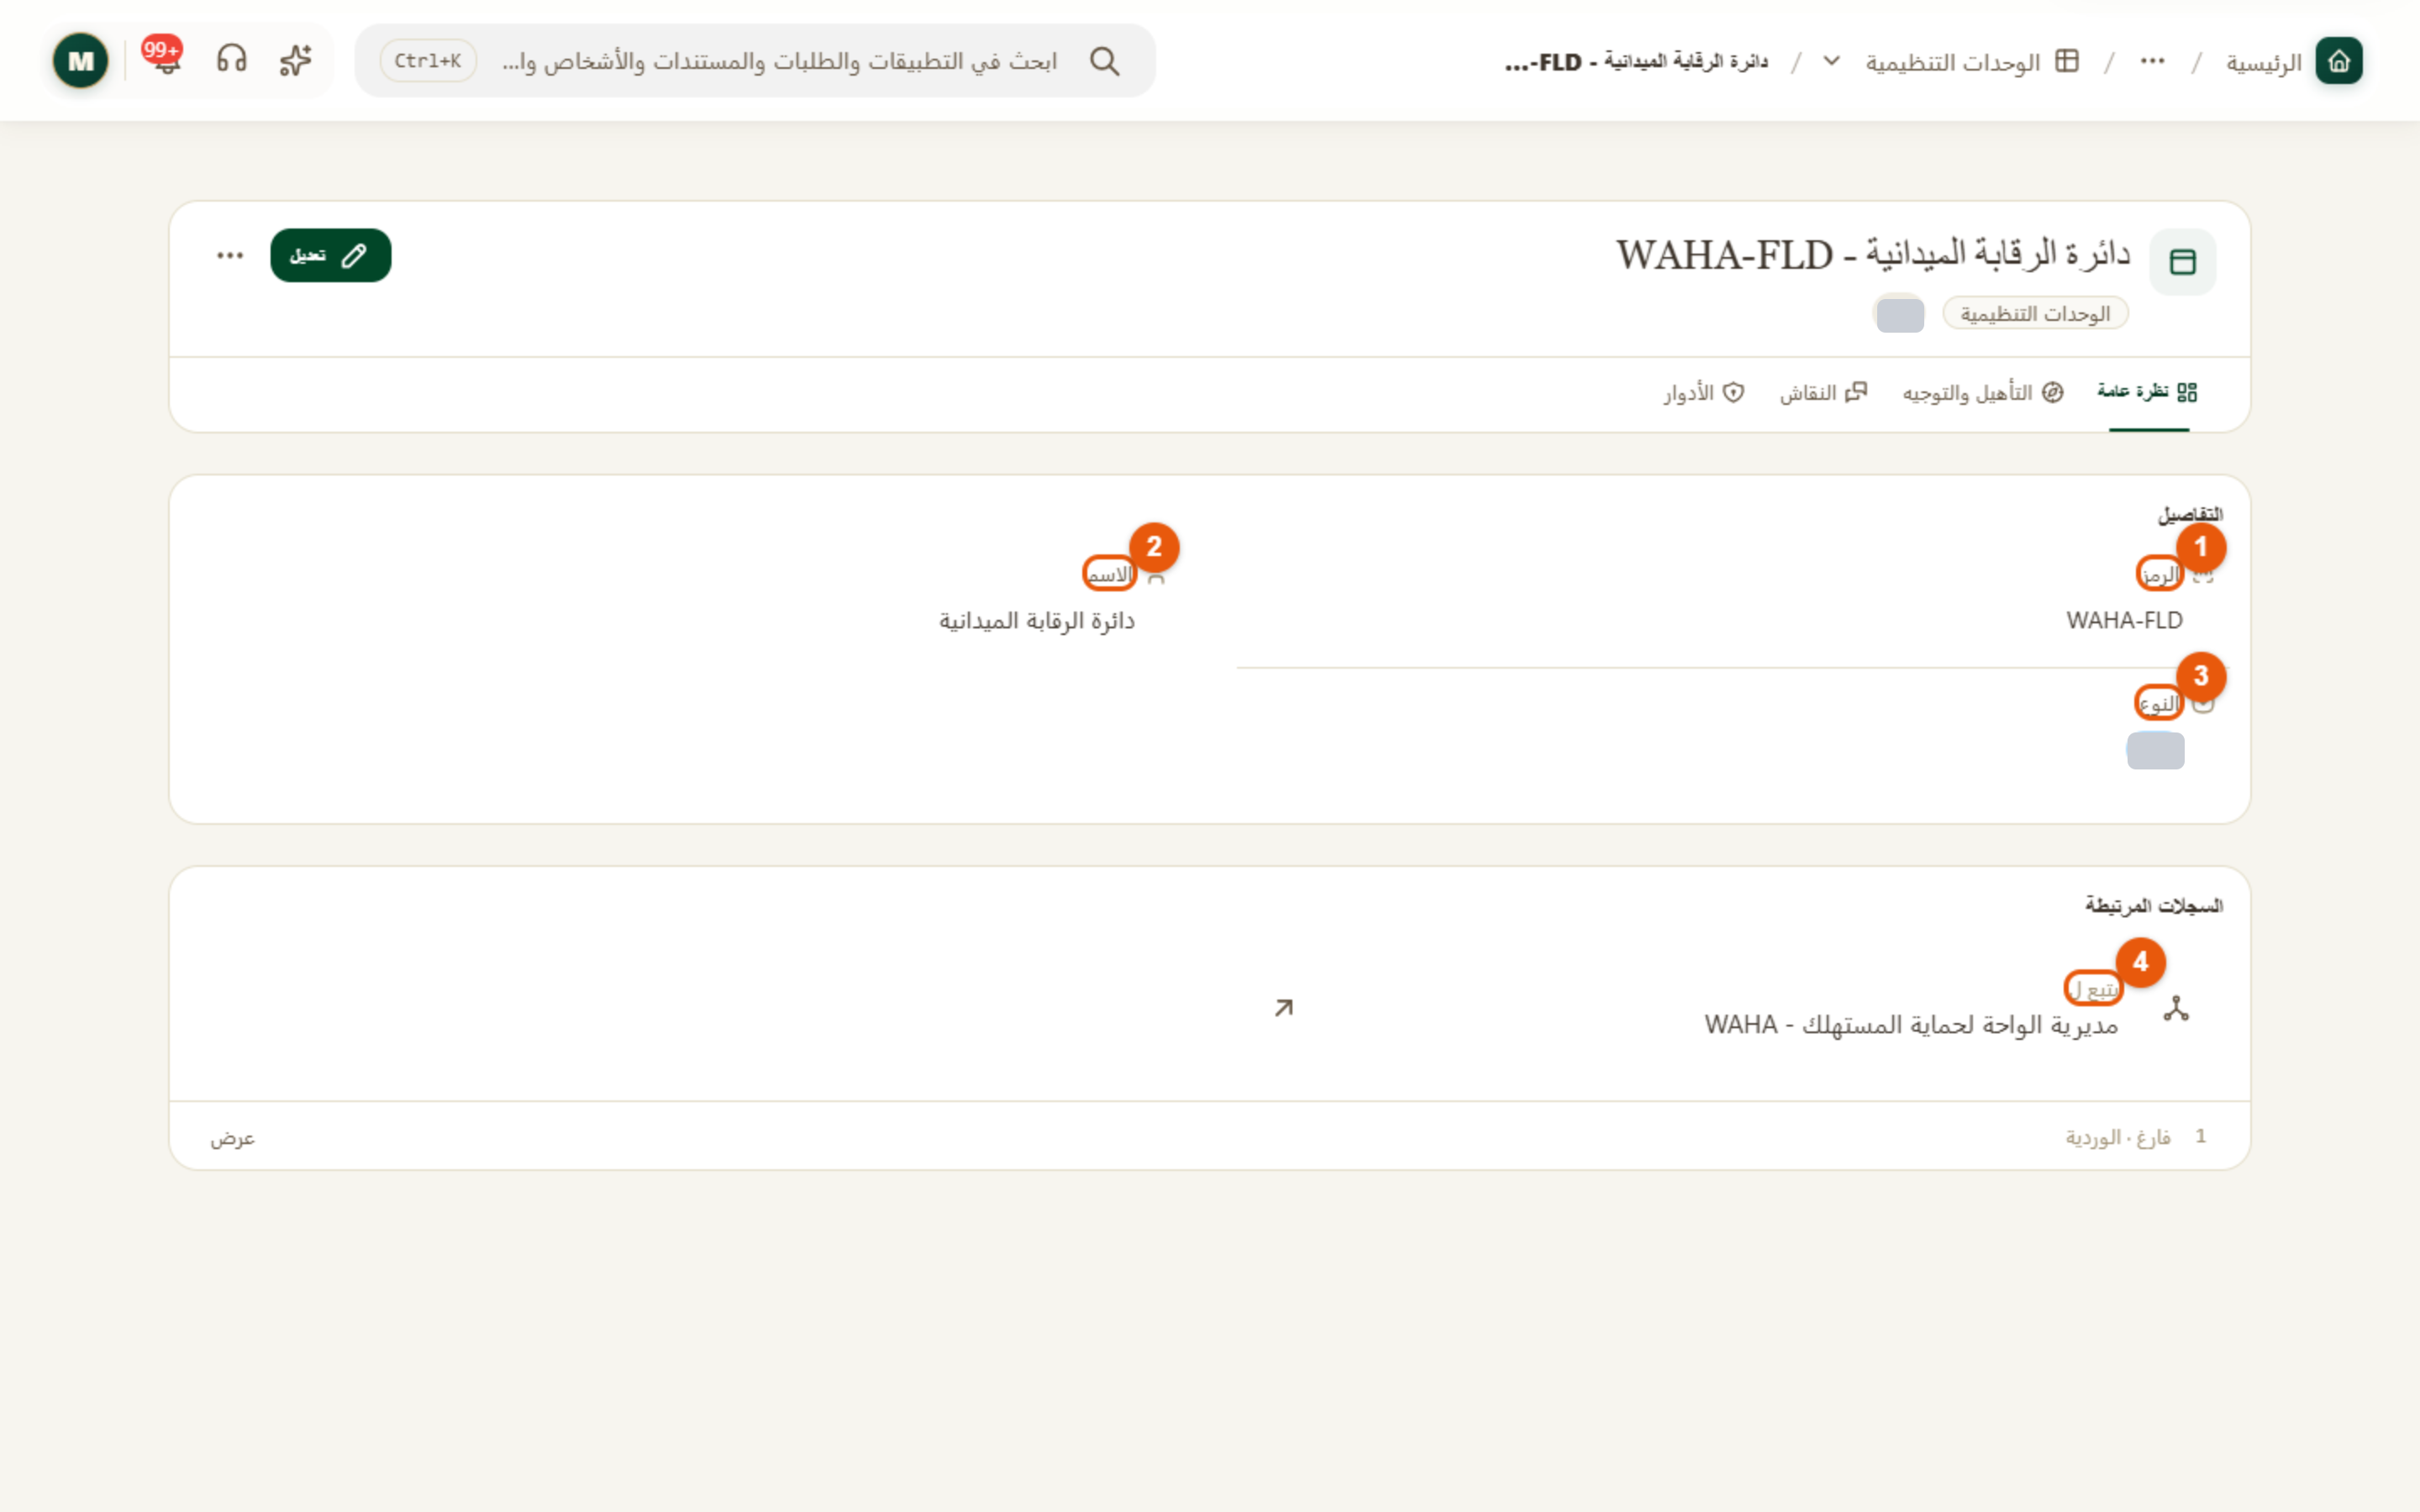
\includegraphics[width=0.95\linewidth]{assets/screens/b-node.png}
\caption{وحدة تنظيمية بعد إنشائها}
\label{fig:build-node}
\shotnote{صورة توضيحية من التنفيذ السابق؛ اتبع العلامات المرقّمة، واستخدم أسماء منظمتك وقيمها الواردة في النص بدلاً من بيانات الصورة. يظهر اسم الوحدة في القوائم مع رمزها، مثل «دائرة حماية المستهلك - DIT-CPSF-CP». وبهذا الشكل ستبحث عنها لاحقاً في كل حقل يرتبط بها. ① «الرمز»: قصير وفريد. ② «الاسم». ③ «النوع»: اختر من قائمة مؤسستك؛ فالقائمة تختلف من مؤسسة إلى أخرى، وقيمتها مخفية في الصورة. ④ «يتبع ل»: الوحدة الأعلى.}
\end{figure}

\subsection{خطوات التنفيذ والحفظ}
إذا كان العنصر موجوداً، افتحه وتابع من خطوة الإعداد التالية بدلاً من إنشاء نسخة مكررة. توضح الخطوات أيضاً طريقة إنشائه عند الحاجة؛ وجوده مسبقاً لا يلغي شرح طريقة بنائه.

أدخل «مديرية حماية المستهلك وسلامة الغذاء» بالرمز \en{DIT-CPSF} ونوع «مديرية»، واربطها بالإدارة العامة \en{MEI-DIT}. ثم أدخل «دائرة حماية المستهلك» بالرمز \en{DIT-CPSF-CP} ونوع «دائرة»، واختر المديرية في «يتبع ل».

\begin{enumerate}
\item افتح «الموارد البشرية» ← «الوحدات التنظيمية»، واضغط «سجل جديد».
\item اكتب «الرمز» و«الاسم»، واختر «النوع»، ثم اضغط «إنشاء».
\item أنشئ الوحدة الثانية بالطريقة نفسها، واختر في «يتبع ل» الوحدة الأولى. اكتب جزءاً من اسمها في مربع البحث، ثم اخترها من القائمة.
\end{enumerate}

\textbf{تحقق:} طابق المسار مع الأسماء والرموز أعلاه. لم يكن للإدارة العامة أب مسجل في البيانات المقروءة؛ فلا تضف تبعية للوزارة اعتماداً على الاسم وحده. إذا اختلف المسار، راجع السجل والرمز مع مسؤول الهيكل.

\section{أنشئ أوصاف الوظائف والمناصب}
\label{sec:build-positions}

الوصف الوظيفي يصف العمل، والمنصب يضع هذا العمل في وحدة تنظيمية ويحدد مديره. توجد أوصاف ومناصب مستقلة للفريق؛ افتحها بدلاً من إنشاء نسخ جديدة.

\begin{rcnote}[من منظمتك: حماية المستهلك]
المناصب الثلاثة في «دائرة حماية المستهلك». يتبع «باحث ميداني — 01» لرئيس فريق الكشف، لكن «مدقق كشوف المنشآت — 01» يتبع لرئيس الدائرة مباشرة. ويتبع رئيس الفريق أيضاً لرئيس الدائرة؛ فلا تجعل المدقق تابعاً لرئيس الفريق عند قراءة المثال.
\end{rcnote}

\begin{table}[H]
\centering
\caption{أوصاف الفريق ومناصبه}
\label{tab:build-positions}
\begin{tabularx}{\linewidth}{R{4.4cm} Y}
\rcHeaderRow
\thh{الوصف الوظيفي ورمزه} & \thh{المنصب ورمزه}\\
رئيس فريق الكشف الميداني؛ \en{JD-CP-FIELD-LEAD} & رئيس فريق الكشف الميداني — 01؛ \en{POS-CP-FIELD-LEAD-01}.\\
باحث ميداني؛ \en{JD-CP-INSPECTOR} & باحث ميداني — 01؛ \en{POS-CP-INSPECTOR-01}.\\
مدقق كشوف المنشآت؛ \en{JD-CP-REVIEWER} & مدقق كشوف المنشآت — 01؛ \en{POS-CP-REVIEWER-01}.\\
\end{tabularx}
\end{table}

\begin{figure}[H]
\centering
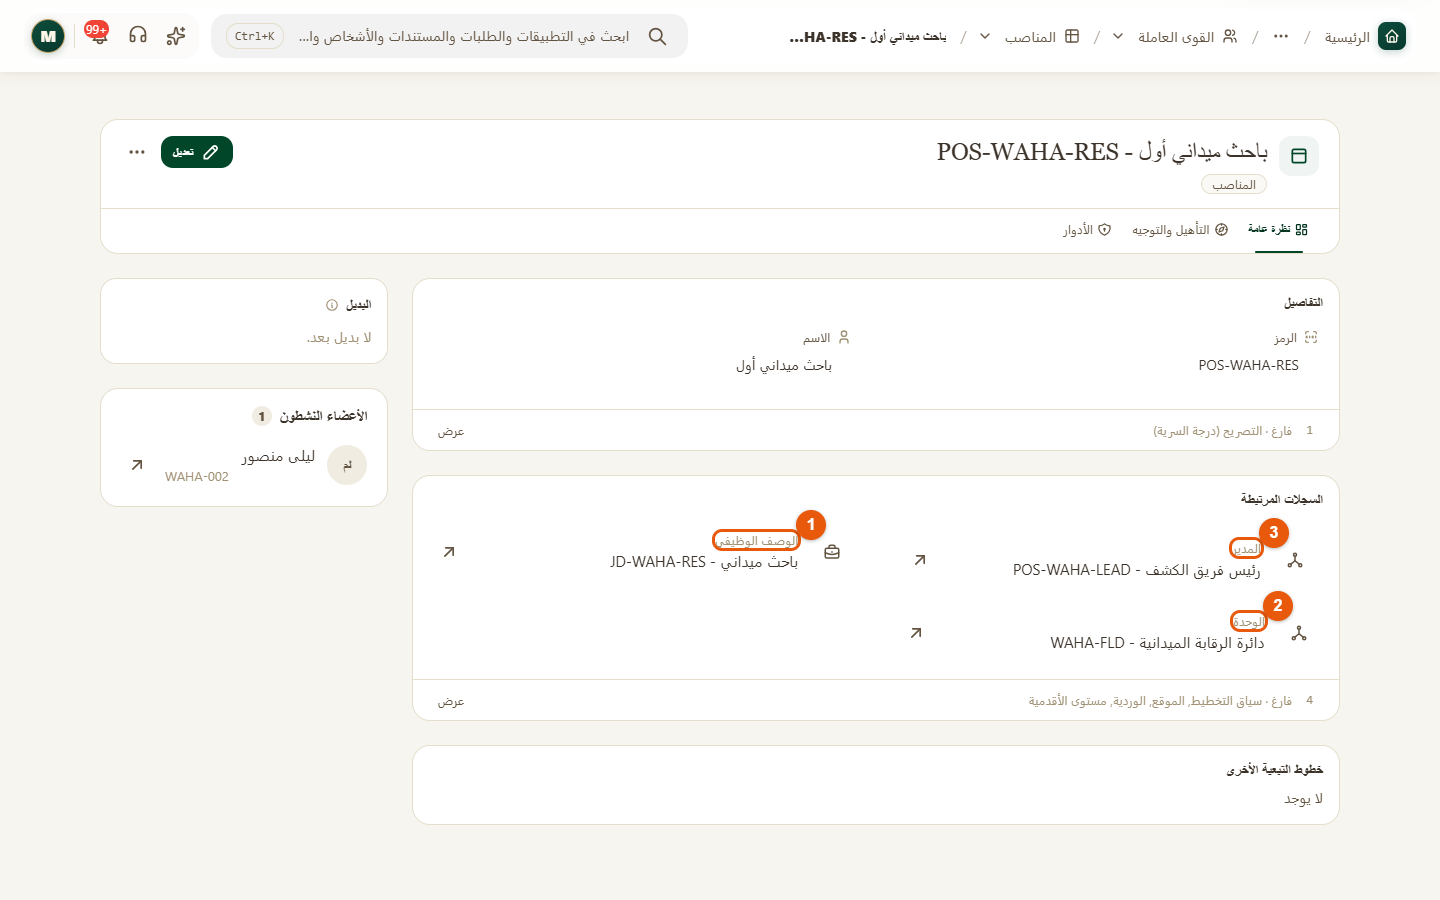
\includegraphics[width=0.95\linewidth]{assets/screens/b-position.png}
\caption{منصب مرتبط بوصفه ووحدته ومديره}
\label{fig:build-position}
\shotnote{صورة توضيحية من التنفيذ السابق؛ اتبع العلامات المرقّمة، واستخدم أسماء منظمتك وقيمها الواردة في النص بدلاً من بيانات الصورة. تجمع صفحة المنصب ارتباطاته، وتعرض «الأعضاء النشطون» فيه بعد التعيين. ① «الوصف الوظيفي». ② «الوحدة»: الدائرة التي يعمل فيها المنصب. ③ «المدير»: المنصب الأعلى، وبه تُبنى التبعية.}
\end{figure}

\subsection{خطوات التنفيذ والحفظ}
إذا كان العنصر موجوداً، افتحه وتابع من خطوة الإعداد التالية بدلاً من إنشاء نسخة مكررة. توضح الخطوات أيضاً طريقة إنشائه عند الحاجة؛ وجوده مسبقاً لا يلغي شرح طريقة بنائه.

استخدم الأوصاف والرموز في الجدول أعلاه. أنشئ رئيس الفريق قبل الباحث، واجعل مدير الباحث «رئيس فريق الكشف الميداني — 01». أما مدير رئيس الفريق ومدقق الكشوف فهو «رئيس دائرة حماية المستهلك»، وليس رئيس الفريق لكليهما.

\begin{enumerate}
\item افتح «الموارد البشرية» ← «وصف الوظيفة» ← «سجل جديد»، واكتب «المسمى الوظيفي» و«الرمز الوظيفي»، ثم اضغط «إنشاء». كرّر ذلك لكل وظيفة.
\item افتح «المناصب» ← «سجل جديد»، واكتب «الرمز» و«الاسم».
\item اختر «الوصف الوظيفي» و«الوحدة»، واختر «المدير» إن وُجد، ثم اضغط «إنشاء».
\end{enumerate}

\textbf{تحقق:} مدير رئيس الفريق والمدقق هو «رئيس دائرة حماية المستهلك» برمز \en{POS-CPSF-CP-H}. إذا ظهر ارتباط مختلف، تحقق من رمز المنصب قبل تعديل العلاقة.

\section{أضف الأعضاء وعيّنهم في مناصبهم}
\label{sec:build-members}

العضو هو الشخص، والتعيين هو العلاقة التي تجعله يشغل منصباً. توجد تعيينات نشطة للأعضاء الثلاثة، ولذلك تبدأ هذه الخطوة بمراجعتها.

\begin{rcnote}[من منظمتك: حماية المستهلك]
الباحث في هذا الشرح هو «نور حسن — تجريبي». استخدم رقم الموظف \en{DEMO-CP-002} للتأكد من الحساب، ثم طابق تعيينه في «باحث ميداني — 01».
\end{rcnote}

\begin{table}[H]
\centering
\caption{الأعضاء والتعيينات النشطة}
\label{tab:build-members}
\begin{tabularx}{\linewidth}{R{4cm} R{3.1cm} Y}
\rcHeaderRow
\thh{العضو} & \thh{رقم الموظف} & \thh{المنصب}\\
أحمد سالم — تجريبي & \en{DEMO-CP-001} & رئيس فريق الكشف الميداني — 01.\\
نور حسن — تجريبي & \en{DEMO-CP-002} & باحث ميداني — 01.\\
ريم خالد — تجريبي & \en{DEMO-CP-003} & مدقق كشوف المنشآت — 01.\\
\end{tabularx}
\end{table}

\begin{figure}[H]
\centering
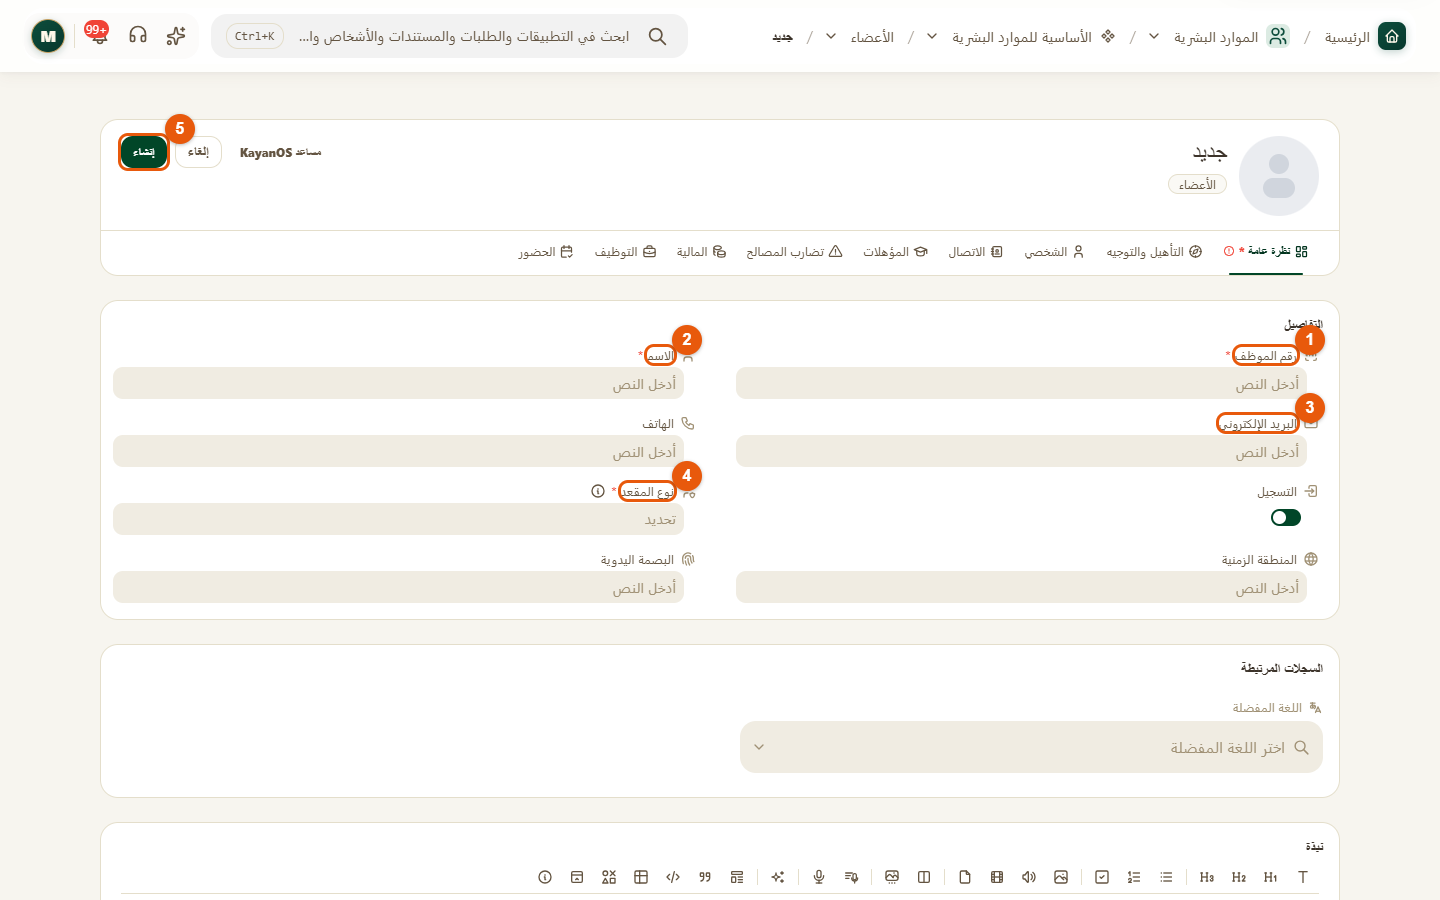
\includegraphics[width=0.95\linewidth]{assets/screens/b-member.png}
\caption{إضافة عضو}
\label{fig:build-member}
\shotnote{صورة توضيحية من التنفيذ السابق؛ اتبع العلامات المرقّمة، واستخدم أسماء منظمتك وقيمها الواردة في النص بدلاً من بيانات الصورة. الحقول المعلّمة بنجمة مطلوبة، وبقية التبويبات تُستكمل لاحقاً. ① «رقم الموظف». ② «الاسم». ③ «البريد الإلكتروني»: عنوان الدخول. ④ «نوع المقعد»: «مقعد كامل» لمن يعمل في النماذج والموافقات. ⑤ «إنشاء».}
\end{figure}

\begin{figure}[H]
\centering
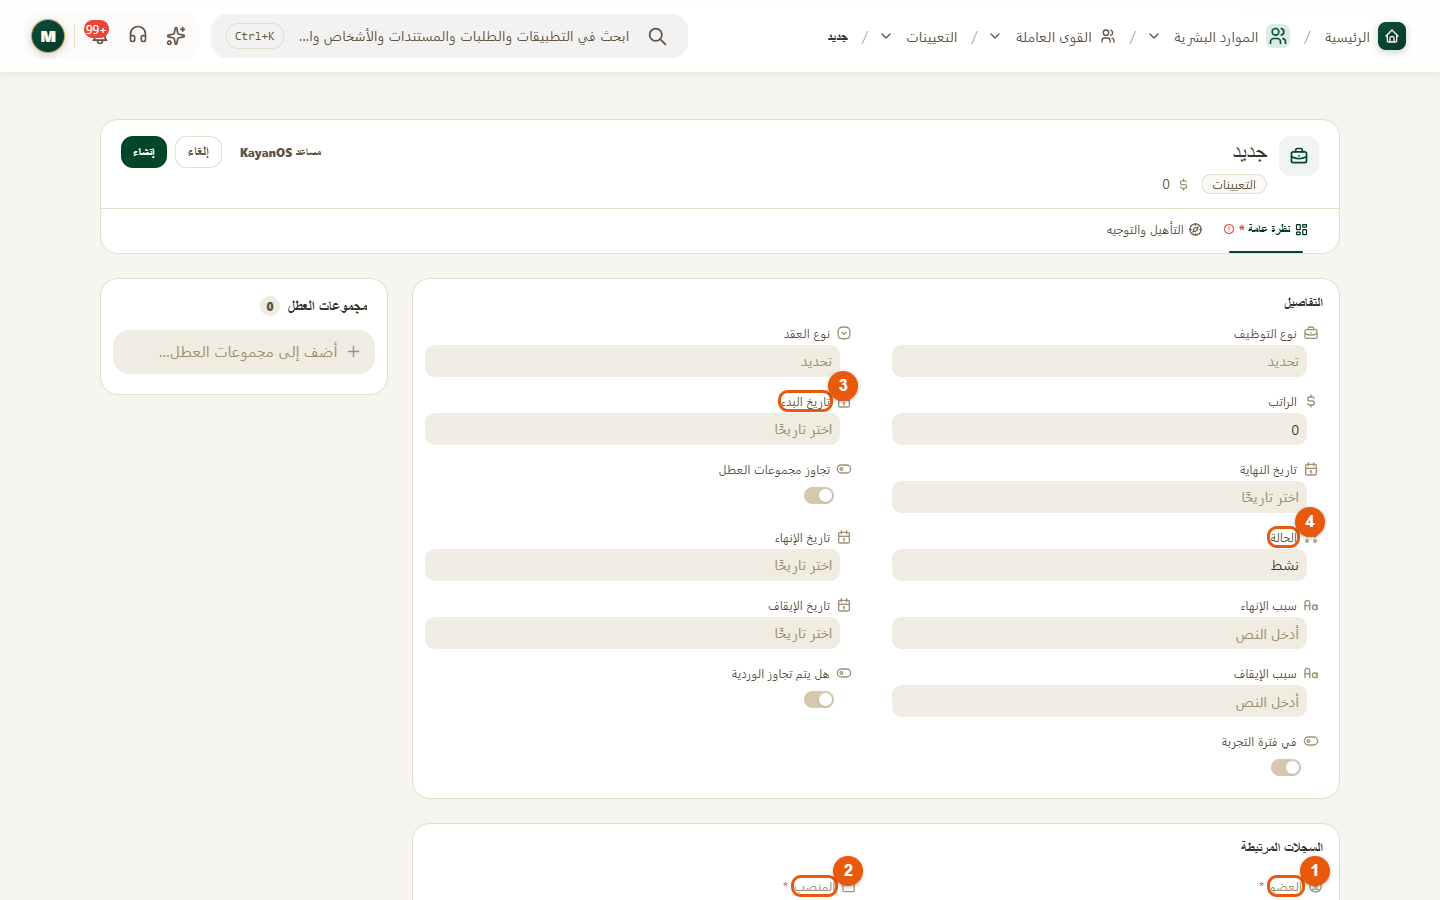
\includegraphics[width=0.95\linewidth]{assets/screens/b-assignment.png}
\caption{إنشاء تعيين}
\label{fig:build-assignment}
\shotnote{صورة توضيحية من التنفيذ السابق؛ اتبع العلامات المرقّمة، واستخدم أسماء منظمتك وقيمها الواردة في النص بدلاً من بيانات الصورة. التعيين سجل مستقل يحفظ تاريخ العلاقة بين الشخص والمنصب. ① «العضو». ② «المنصب». ③ «تاريخ البدء». ④ «الحالة»: تبدأ «نشط».}
\end{figure}

\subsection{خطوات التنفيذ والحفظ}
إذا كان العنصر موجوداً، افتحه وتابع من خطوة الإعداد التالية بدلاً من إنشاء نسخة مكررة. توضح الخطوات أيضاً طريقة إنشائه عند الحاجة؛ وجوده مسبقاً لا يلغي شرح طريقة بنائه.

استخدم الأسماء وأرقام الموظفين في الجدول أعلاه. عند إنشاء تعيين، اختر العضو ومنصبه المقابل في الصف نفسه، وأدخل تاريخ البدء الفعلي. لا تستخدم بريداً إلكترونياً أو كلمة مرور افتراضية من دليل التدريب.

\begin{enumerate}
\item افتح «الموارد البشرية» ← «الأعضاء» ← «سجل جديد»، واملأ الحقول المطلوبة، ثم اضغط «إنشاء».
\item افتح «التعيينات» ← «سجل جديد»، واختر «العضو» ثم «المنصب»، ثم اضغط «إنشاء». ويبقى النموذج مفتوحاً بعد الحفظ؛ فافتح «سجل جديد» من القائمة قبل التعيين التالي.
\end{enumerate}

\textbf{تحقق:} طابق كل صف في الجدول مع تعيينه. إذا لم يظهر التعيين، راجع حالته وتواريخه مع المسؤول؛ ولا تغيّر كلمة مرور العضو لأجل متابعة الدليل.

\section{اضبط المجموعات والأدوار}
\label{sec:build-roles}

المجموعة تجمع المشاركين، أما الدور فيحمل صلاحيات ضمن نطاق محدد. وجود مجموعة لا يثبت وحده أن أعضاءها يستطيعون فتح نموذج أو اعتماد كشف.

\begin{rcnote}[من منظمتك: حماية المستهلك]
توجد مجموعة «فريق الكشف الميداني — 01» برمز \en{GRP-CP-FIELD-01}، ومجموعة «مدققو كشوف المنشآت» برمز \en{GRP-CP-REVIEWERS}. ويوجد دور «مراقب حماية المستهلك» على مستوى المنظمة، ودور «مدقق كشوف المنشآت» ضمن النموذج \en{001}؛ وهما نطاقان مختلفان.
\end{rcnote}

\begin{figure}[H]
\centering
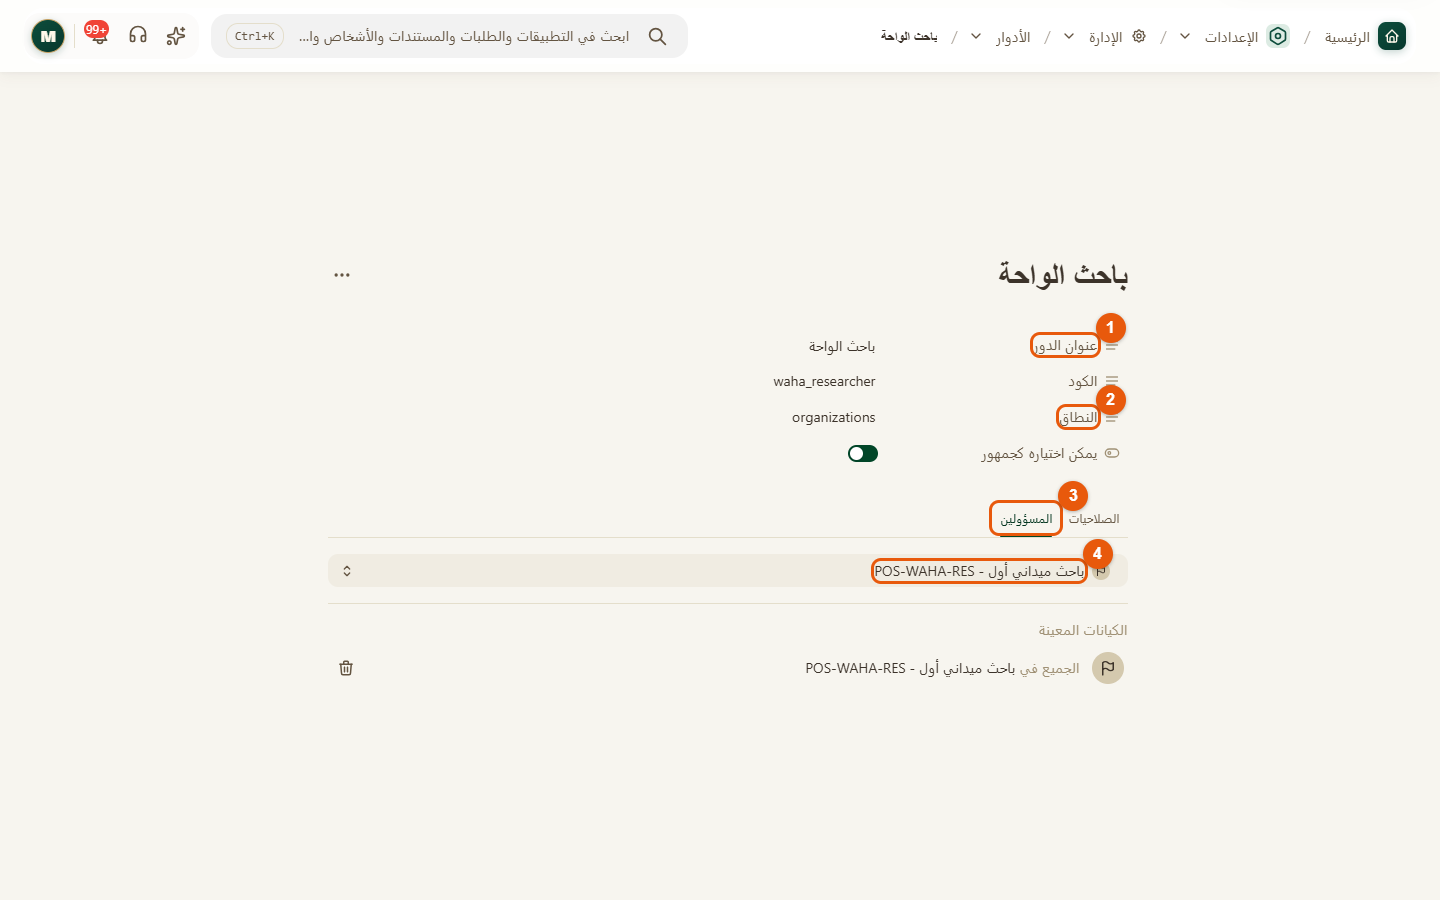
\includegraphics[width=0.95\linewidth]{assets/screens/b-role.png}
\caption{دور مسنَد إلى منصب}
\label{fig:build-role}
\shotnote{صورة توضيحية من التنفيذ السابق؛ اتبع العلامات المرقّمة، واستخدم أسماء منظمتك وقيمها الواردة في النص بدلاً من بيانات الصورة. يُحفظ الإسناد فور اختياره، ويظهر تحت «الكيانات المعينة». أما الصلاحيات نفسها فتُمنح لاحقاً من نوع السجلات. ① «عنوان الدور». ② «النطاق»: «المنظمات» يعني المؤسسة كلها. ③ «المسؤولين». ④ المنصب الذي يحمل الدور.}
\end{figure}

\subsection{خطوات التنفيذ والحفظ}
إذا كان العنصر موجوداً، افتحه وتابع من خطوة الإعداد التالية بدلاً من إنشاء نسخة مكررة. توضح الخطوات أيضاً طريقة إنشائه عند الحاجة؛ وجوده مسبقاً لا يلغي شرح طريقة بنائه.

للمجموعات استخدم «فريق الكشف الميداني — 01» ورمز \en{GRP-CP-FIELD-01}، و«مدققو كشوف المنشآت» ورمز \en{GRP-CP-REVIEWERS}. للأدوار افتح «مراقب حماية المستهلك» الموجود على مستوى المنظمة، وراجع دور «مدقق كشوف المنشآت» داخل النموذج؛ لا تنشئ دوراً بنفس الاسم في نطاق آخر.

\begin{enumerate}
\item للمجموعة: افتح «الموارد البشرية» ← «المجموعات» ← «سجل جديد»، واكتب «الرمز» و«الاسم»، واختر في «نوع المجموعة» «يدوي».
\item للدور: افتح «الإعدادات» ← «الأدوار» ← «إضافة الدور»، وافتح الدور الموجود في نطاقه الصحيح. ولإنشاء دور ناقص ومعتمد، اكتب «عنوان الدور» و«الكود»، ثم اضغط «إنشاء الدور».
\item في صفحة الدور افتح «المسؤولين» ← «تعيين الأعضاء والمناصب والعقد»، وابحث عن المنصب واختره.
\end{enumerate}

\textbf{تحقق:} فرّق بين المجموعة والدور والمنصب. إذا لم تجد إسناداً، فراجع مسؤول الصلاحيات؛ ولا تنشئ أدواراً جديدة لمجرد اتباع الشرح.

\section{اضبط التطبيق ونوع السجلات}
\label{sec:build-entity}

التطبيق يجمع صفحات العمل، والقسم ينظمها، ونوع السجلات يحدد البيانات المحفوظة. قد تحمل هذه العناصر أسماء متقاربة، لكنها ليست سجلاً واحداً.

\begin{rcnote}[من منظمتك: حماية المستهلك]
النموذج «كشف منشأة تجارية لطلب سجل تجاري» موجود حالياً في «حماية المستهلك» ← «السجلات». ويوجد أيضاً تطبيق «السجلات التجارية» وفيه قسم اسمه حرفياً «المنشآات التجارية». أما اسم نوع السجلات فهو «المنشآت التجارية»؛ انتبه إلى اختلاف كتابة اسم القسم عن نوع السجلات.
\end{rcnote}

\begin{figure}[H]
\centering
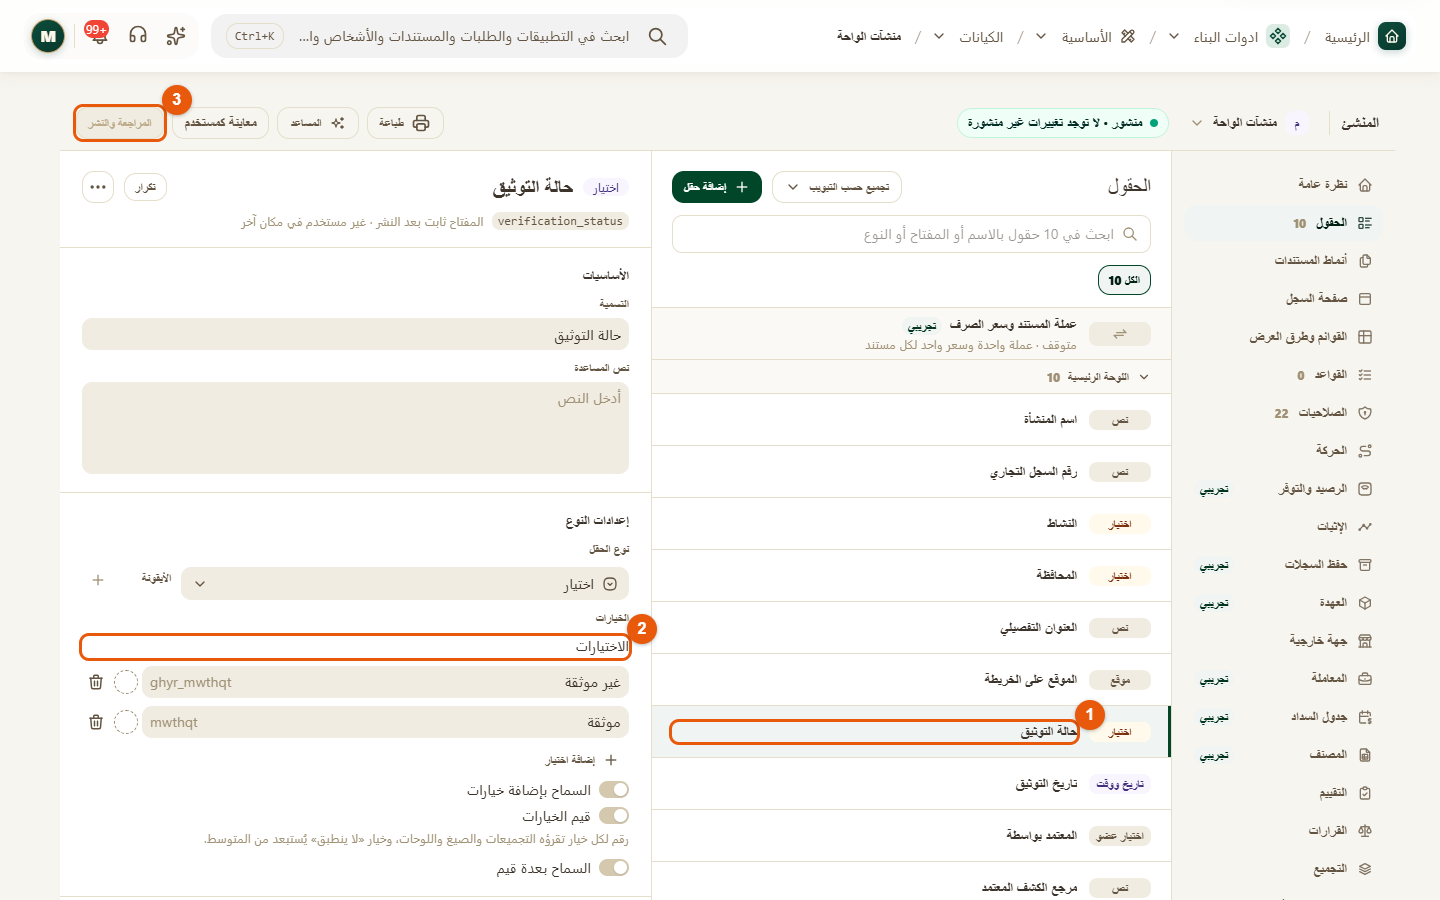
\includegraphics[width=0.95\linewidth]{assets/screens/b-entity-fields.png}
\caption{حقل اختيار ومفاتيح خياراته}
\label{fig:build-entity-fields}
\shotnote{صورة توضيحية من التنفيذ السابق؛ اتبع العلامات المرقّمة، واستخدم أسماء منظمتك وقيمها الواردة في النص بدلاً من بيانات الصورة. يحفظ النظام كل خيار بمفتاح يولّده من نصه بحروف لاتينية، فيُحفظ «موثقة» بالمفتاح mwthqt و«دمشق» بالمفتاح dmshq. وستحتاج إلى هذا المفتاح، لا إلى النص، في القيم الافتراضية والقواعد. ① الحقل المحدد. ② «الاختيارات»: يظهر المفتاح بجانب كل خيار. ③ «المراجعة والنشر».}
\end{figure}

\subsection{خطوات التنفيذ والحفظ}
إذا كان العنصر موجوداً، افتحه وتابع من خطوة الإعداد التالية بدلاً من إنشاء نسخة مكررة. توضح الخطوات أيضاً طريقة إنشائه عند الحاجة؛ وجوده مسبقاً لا يلغي شرح طريقة بنائه.

استخدم التطبيق «حماية المستهلك» والقسم «السجلات» للنموذج. نوع السجلات هو «المنشآت التجارية»؛ عند استكمال حقوله، احتفظ بالحقول والمفاتيح الموجودة ولا تستبدلها بحقول المثال المصوّر. افتح «فرن الأمانة» كسجل المثال الموجود.

\begin{enumerate}
\item افتح «ادوات البناء» ← «التطبيقات» ← «سجل جديد»، واملأ «العنوان» و«الوصف» و«الأيقونة»، ثم اضغط «إنشاء». والأيقونة اسم إنجليزي قصير مثل \en{shield}.
\item افتح «أقسام التطبيق» ← «سجل جديد»، واكتب «العنوان» و«الوصف» و«الأيقونة»، واختر «التطبيق»، ثم اضغط «إنشاء».
\item افتح «الكيانات» ← «إضافة كيان»، واكتب «عنوان الكيان» والوصف.
\item اضغط «حقل 1» لتفتح «إعدادات الحقل» على الجانب، واختر النوع، واكتب العنوان والمفتاح بحروف إنجليزية. ثم اضغط «اضافة حقل جديد» لكل حقل آخر، و«إضافة اختيار» لكل خيار.
\item اضغط «إعدادات الكيان»، واختر في «حقول الاسم المعروض» «اسم المنشأة»، وفعّل «إظهار في التنقل»، واختر «التطبيق» و«قسم التطبيق»، ثم اضغط «انشاء كيان».
\item افتح التطبيق، واضغط «سجل جديد» تحت «المنشآت التجارية»، واستخدم بيانات المنشأة الفعلية عند الحاجة إلى إضافة سجل ناقص؛ وإذا كانت «فرن الأمانة» موجودة فافتحها.
\end{enumerate}

\textbf{تحقق:} تأكد من نوع السجلات ومفتاحه. وجود قسم باسم المنشآت لا يثبت مكان ظهور النوع؛ إذا لم تجده في التنقل، راجع إعدادات إظهاره وصلاحيات الحساب.

\section{امنح صلاحيات الوصول إلى المنشآت}
\label{sec:build-grants}

صلاحية النموذج وصلاحية نوع السجلات مسألتان منفصلتان. قد يتمكن عضو من فتح الكشف ولا يتمكن من قراءة المنشأة المرتبطة به.

\begin{rcnote}[من منظمتك: حماية المستهلك]
ابدأ من دور «مراقب حماية المستهلك» عند تتبّع وصول الفريق إلى المنشآت. ولا تفترض أن دور «مدقق كشوف المنشآت» ضمن النموذج يمنح تلقائياً الوصول إلى «المنشآت التجارية».
\end{rcnote}

\begin{figure}[H]
\centering
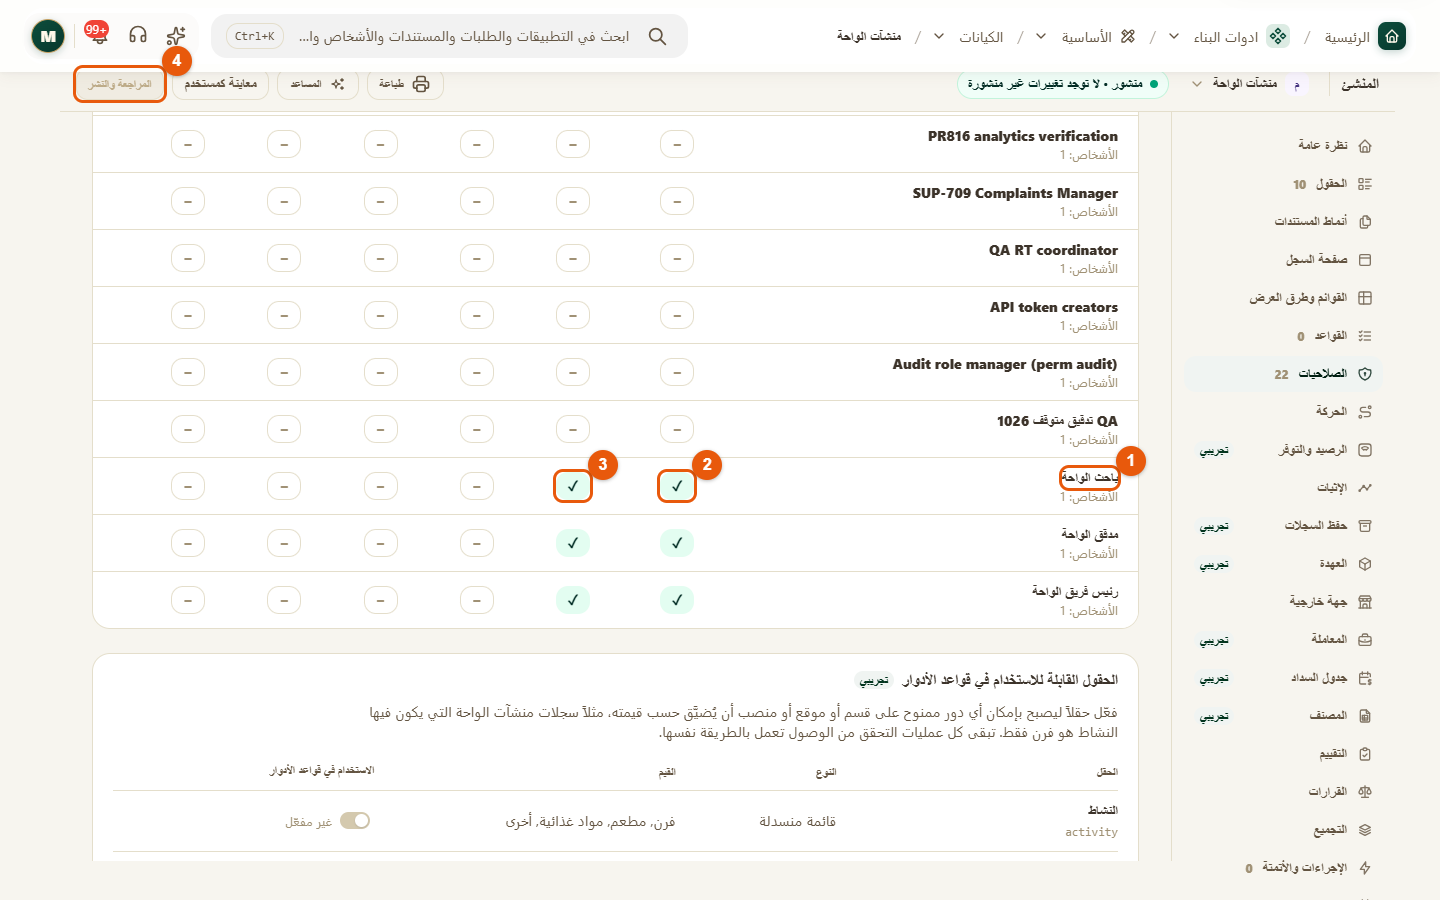
\includegraphics[width=0.95\linewidth]{assets/screens/b-grants.png}
\caption{صلاحيات الأدوار على نوع السجلات}
\label{fig:build-grants}
\shotnote{صورة توضيحية من التنفيذ السابق؛ اتبع العلامات المرقّمة، واستخدم أسماء منظمتك وقيمها الواردة في النص بدلاً من بيانات الصورة. كل صف دور، وكل عمود فعل. ويُظهر الصف عدد الأشخاص الذين يحملون الدور، وهو دليل على صحة الإسناد إلى المنصب. ① الدور. ② «قائمة». ③ «فتح». ④ «المراجعة والنشر»: يعرض التغييرات قبل نشرها.}
\end{figure}

\subsection{خطوات التنفيذ والحفظ}
إذا كان العنصر موجوداً، افتحه وتابع من خطوة الإعداد التالية بدلاً من إنشاء نسخة مكررة. توضح الخطوات أيضاً طريقة إنشائه عند الحاجة؛ وجوده مسبقاً لا يلغي شرح طريقة بنائه.

\begin{enumerate}
\item افتح «الكيانات» ← نوع السجلات ← «الصلاحيات» ← «الأدوار».
\item اضغط «قائمة» و«فتح» في صف كل دور.
\item اضغط «المراجعة والنشر»، ثم «نشر».
\end{enumerate}

\textbf{تحقق:} يستطيع العضو المخوّل فتح القائمة والسجل المطلوب. إذا لم يستطع، راجع الإسناد والنطاق والنشر، ولا تستنتج أن السجل غير موجود.

\section{اضبط نموذج الكشف واربطه بالمنشأة}
\label{sec:build-form}

استخدم النموذج الموجود. الاسم أو ظهور سؤال منشأة لا يكفيان لإثبات أن الحقول تُقرأ أو تُكتب؛ يجب مراجعة الربط داخل المحرر.

\begin{rcnote}[من منظمتك: حماية المستهلك]
اسم النموذج هو «كشف منشأة تجارية لطلب سجل تجاري»، ومعرّفه \en{001}. اختر هذا النموذج تحديداً، ونوع السجلات «المنشآت التجارية» عند فحص سؤال المنشأة.
\end{rcnote}

\begin{figure}[H]
\centering
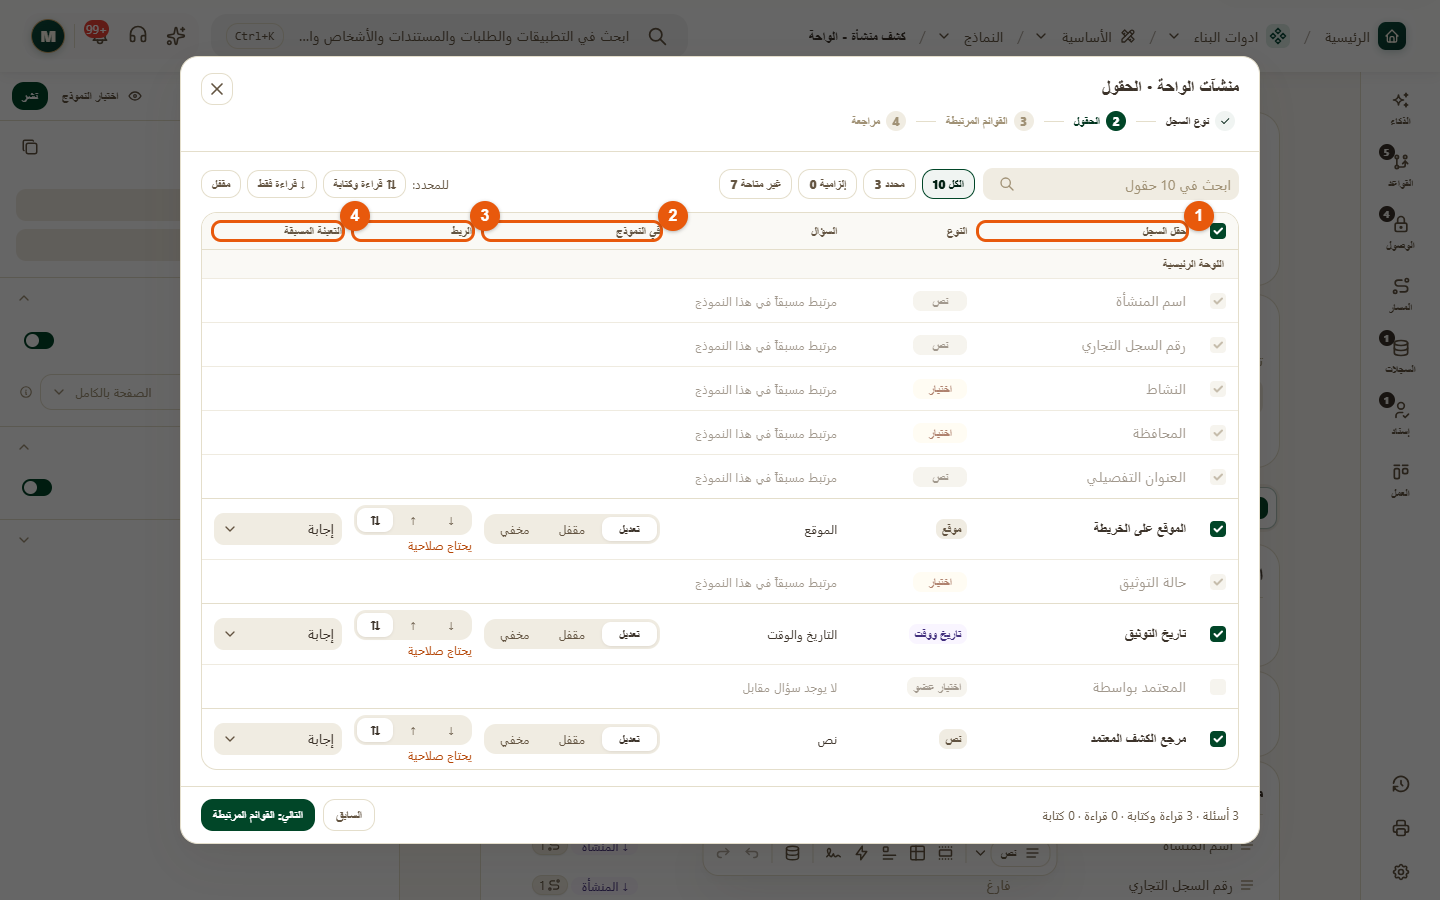
\includegraphics[width=0.95\linewidth]{assets/screens/b-wizard.png}
\caption{معالج «إضافة أسئلة من نوع سجل»}
\label{fig:build-wizard}
\shotnote{صورة توضيحية من التنفيذ السابق؛ اتبع العلامات المرقّمة، واستخدم أسماء منظمتك وقيمها الواردة في النص بدلاً من بيانات الصورة. يعرض كل صف حقلاً من المنشأة، ويحدد ما يحدث له في النموذج. ① «حقل السجل». ② «في النموذج»: «تعديل» أو «مقفل» أو «مخفي». ③ «الربط»: ↓ قراءة، ↑ كتابة، ⇅ الاثنان. ④ «التعبئة المسبقة».}
\end{figure}

\begin{figure}[H]
\centering
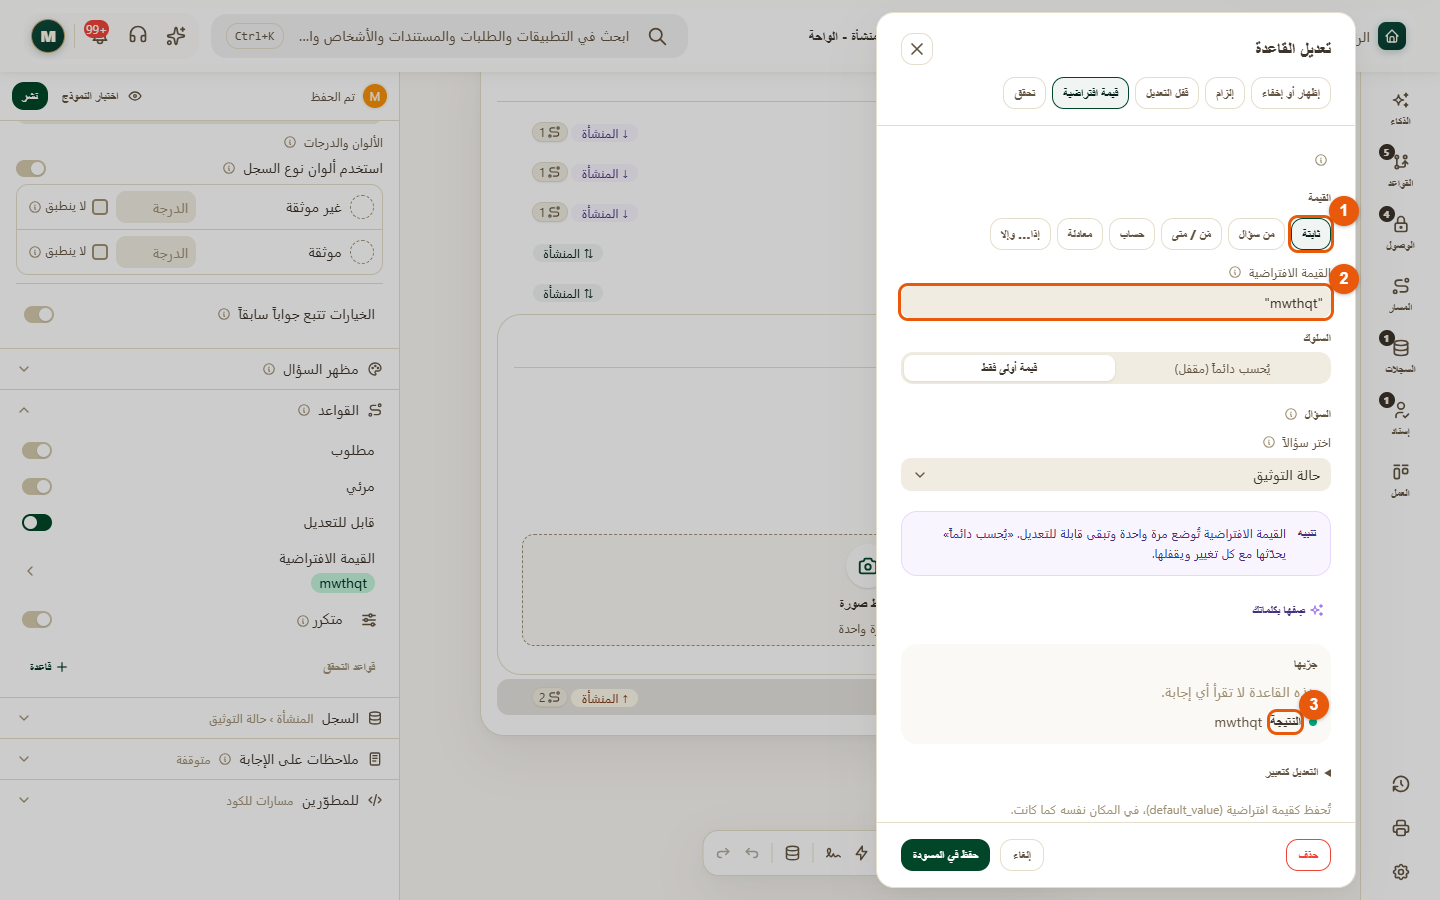
\includegraphics[width=0.85\linewidth]{assets/screens/b-default.png}
\caption{قيمة افتراضية لسؤال مخفي}
\label{fig:build-default}
\shotnote{صورة توضيحية من التنفيذ السابق؛ اتبع العلامات المرقّمة، واستخدم أسماء منظمتك وقيمها الواردة في النص بدلاً من بيانات الصورة. القيمة هنا تعبير، لذلك يُكتب النص بين علامتي تنصيص. ويجب أن يكون مفتاح الخيار، لا نصه الظاهر. ① «ثابتة». ② «القيمة الافتراضية»: \en{"mwthqt"}. ③ «النتيجة»: تتحقق منها قبل الحفظ.}
\end{figure}

\subsection{خطوات التنفيذ والحفظ}
إذا كان العنصر موجوداً، افتحه وتابع من خطوة الإعداد التالية بدلاً من إنشاء نسخة مكررة. توضح الخطوات أيضاً طريقة إنشائه عند الحاجة؛ وجوده مسبقاً لا يلغي شرح طريقة بنائه.

افتح النموذج الموجود «كشف منشأة تجارية لطلب سجل تجاري» ومعرّفه \en{001}. اختر «المنشآت التجارية» مصدراً للسؤال. حدّد لكل حقل القراءة والكتابة وفق إجراء العمل؛ مفاتيح الخيارات في الصورة أمثلة، ويجب نسخ المفتاح الفعلي من حقلك.

\begin{enumerate}
\item افتح «ادوات البناء» ← «النماذج» ← «إنشاء نموذج». اكتب الاسم و«كود النموذج» و«الاختصار المرجعي»، مثل \en{KSHF}، فتحمل الكشوف أرقاماً مثل \en{KSHF-1}. ثم اختر التطبيق والقسم، واضغط «إنشاء».
\item افتح «السجلات» في الشريط الجانبي، واضغط «سؤال سجل»، واختر في «نوع السجل» «المنشآت التجارية». وسمِّ السؤال «المنشأة».
\item افتح «السجلات» مرة أخرى، واضغط «من نوع سجل». اختر نوع السجلات، ثم استخدم سؤال «المنشأة» الموجود، وحدّد الحقول وطريقة ربطها، ثم اضغط «إضافة».
\item أضف أسئلة الكشف من الشريط السفلي: «اختر نوع الحقل» يضيف سؤالاً جديداً من النوع الذي تختاره، ولا يغيّر نوع السؤال المحدد.
\item حدّد سؤال «حالة التوثيق»، ثم «القواعد» ← «القيمة الافتراضية» ← «ثابتة»، واكتب مفتاح الخيار الفعلي بين علامتي تنصيص؛ القيمة المصوّرة مثال فقط. وتأكد من أن «متكرر» متوقف.
\end{enumerate}

\textbf{تحقق:} في المعاينة، يجب أن يشير اختيار «فرن الأمانة» إلى السجل الموجود، لا إلى نص حر بالاسم نفسه. اقرأ مفاتيح الخيارات والقيم الافتراضية من إعداد الحقل الحالي، ولا تنقلها من مثال آخر.

\section{اسمح للنموذج بالكتابة إلى المنشأة}
\label{sec:build-allow}

القراءة من المنشأة لا تعني السماح للنموذج بتعديلها. إذا كان النموذج مصمماً للكتابة، فراجع الحقول المسموح بها وتوقيت تطبيق التغييرات.

\begin{rcnote}[من منظمتك: حماية المستهلك]
راجع السماح الخاص بـ«كشف منشأة تجارية لطلب سجل تجاري» على «المنشآت التجارية». لا ينسب هذا الفصل إلى المنظمة حالة «مسموح» أو تحديثاً ناجحاً؛ فذلك يحتاج إلى فحص الإعداد وتشغيل كشف مخوّل.
\end{rcnote}

\begin{figure}[H]
\centering
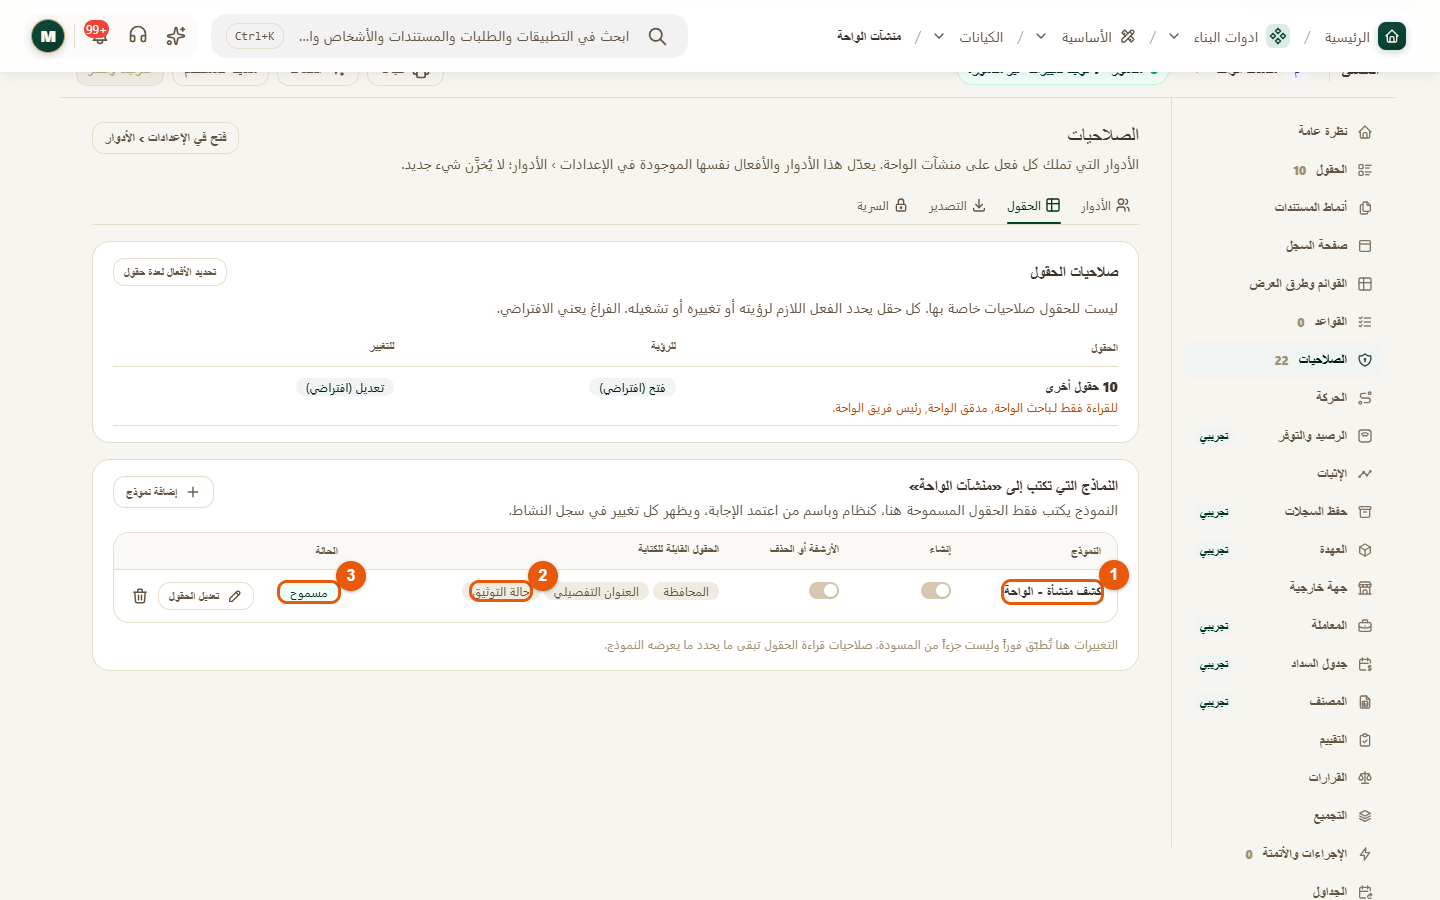
\includegraphics[width=0.95\linewidth]{assets/screens/b-form-writes.png}
\caption{«النماذج التي تكتب إلى «المنشآت التجارية»»}
\label{fig:build-allow}
\shotnote{صورة توضيحية من التنفيذ السابق؛ اتبع العلامات المرقّمة، واستخدم أسماء منظمتك وقيمها الواردة في النص بدلاً من بيانات الصورة. يكتب النموذج الحقول المسموح بها هنا فقط، ويُسجَّل كل تغيير باسم من اعتمد الإجابة. ① النموذج. ② «الحقول القابلة للكتابة». ③ «الحالة»: «مسموح» بعد الموافقة.}
\end{figure}

\subsection{خطوات التنفيذ والحفظ}
إذا كان العنصر موجوداً، افتحه وتابع من خطوة الإعداد التالية بدلاً من إنشاء نسخة مكررة. توضح الخطوات أيضاً طريقة إنشائه عند الحاجة؛ وجوده مسبقاً لا يلغي شرح طريقة بنائه.

\begin{enumerate}
\item في لوحة «السجلات» داخل النموذج، اضغط «السماح في نوع السجل».
\item راجع الحقول، ثم اضغط «موافقة».
\end{enumerate}

\textbf{تحقق:} يجب أن تتفق حالة السماح والحقول مع غرض النموذج. إذا لم يوجد طلب كتابة، راجع الربط أولاً، بدلاً من افتراض أن اعتماد الكشف سيعدّل المنشأة.

\section{اضبط المسار وخطوة التدقيق}
\label{sec:build-journey}

المسار يحدد حالات الكشف، وخطوة الموافقة تحدد من يتخذ القرار وما يترتب عليه. اقرأ أسماء الحالات والنتائج من النموذج الحالي قبل تفسير القرار.

\begin{rcnote}[من منظمتك: حماية المستهلك]
المنصب الذي يطابق وظيفة التدقيق هو «مدقق كشوف المنشآت — 01»، وتشغله «ريم خالد — تجريبي». ويوجد دور باسم «مدقق كشوف المنشآت» ضمن النموذج؛ لكن وجود الدور والتعيين لا يثبت وحده أن خطوة الموافقة مسندة إليهما.
\end{rcnote}

\begin{figure}[H]
\centering
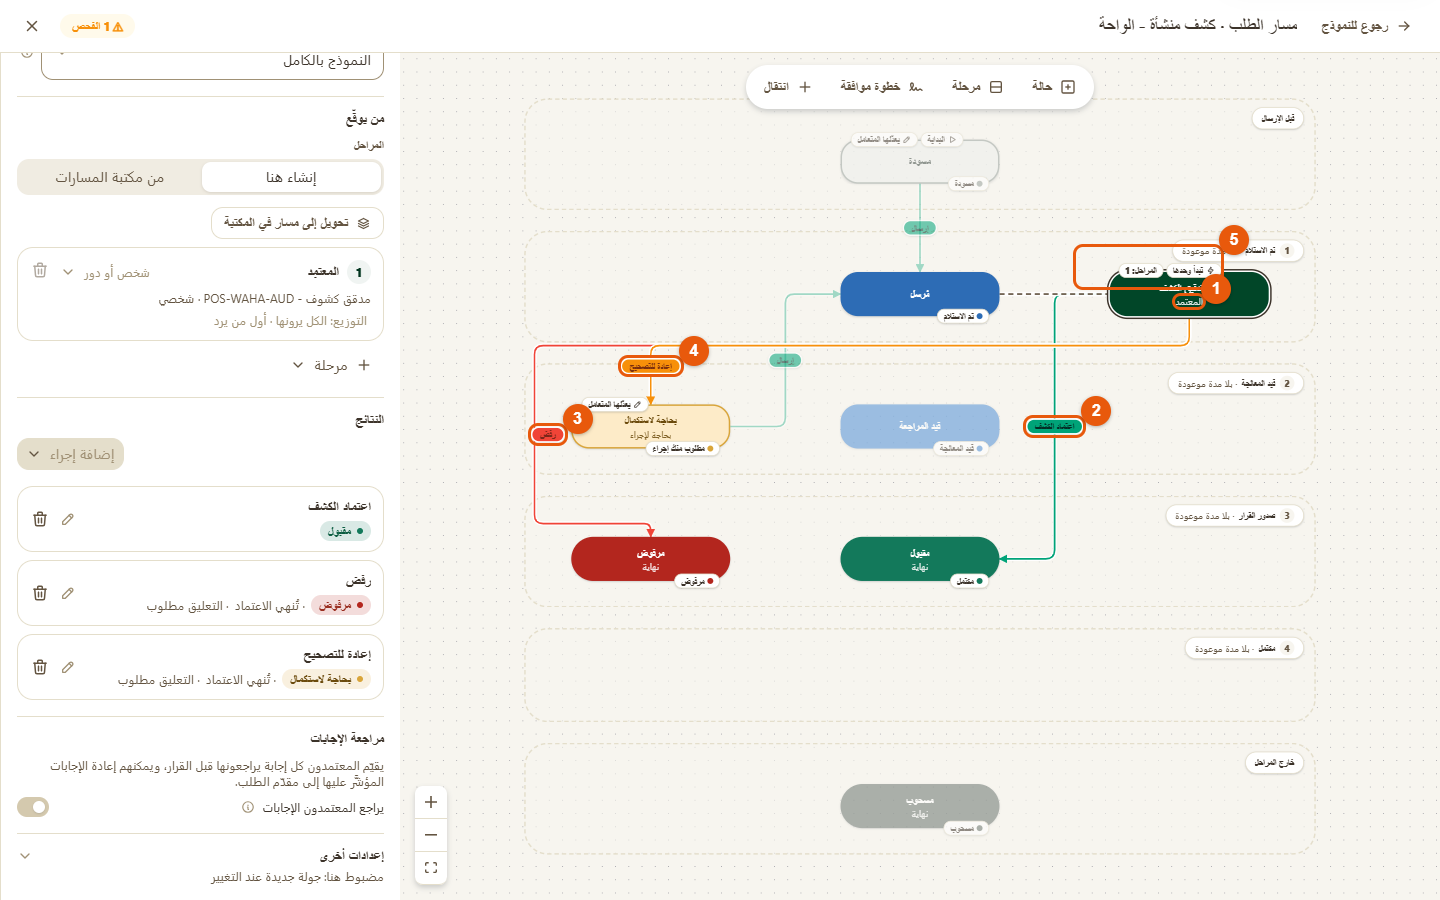
\includegraphics[width=0.95\linewidth]{assets/screens/b-journey.png}
\caption{خطوة الموافقة ونتائجها الثلاث}
\label{fig:build-journey}
\shotnote{صورة توضيحية من التنفيذ السابق؛ اتبع العلامات المرقّمة، واستخدم أسماء منظمتك وقيمها الواردة في النص بدلاً من بيانات الصورة. تظهر كل نتيجة على الخريطة سهماً بلونها. وإذا بقيت النتيجة «تبقى الحالة»، فلن يتغير الكشف بعد القرار. ① المنصب الذي يوقّع. ② «اعتماد الكشف» إلى «مقبول». ③ «رفض» إلى «مرفوض»، والتعليق مطلوب. ④ «إعادة للتصحيح» إلى «بحاجة لاستكمال». ⑤ الخطوة على الخريطة.}
\end{figure}

\subsection{خطوات التنفيذ والحفظ}
إذا كان العنصر موجوداً، افتحه وتابع من خطوة الإعداد التالية بدلاً من إنشاء نسخة مكررة. توضح الخطوات أيضاً طريقة إنشائه عند الحاجة؛ وجوده مسبقاً لا يلغي شرح طريقة بنائه.

اختر «مدقق كشوف المنشآت — 01» عند إعداد الموقّع إذا كان هذا هو الإسناد المعتمد للعمل. أسماء «اعتماد الكشف» و«رفض» و«إعادة للتصحيح» في الشرح تبيّن طريقة ضبط النتائج؛ احتفظ بأسماء النتائج والحالات الموجودة إذا كانت معدّة بالفعل.

\begin{enumerate}
\item افتح «المسار» ← «تفعيل المسار»، ثم «تفعيل خطوات الموافقة»، ثم «خطوة موافقة».
\item اكتب الاسم. ثم اضغط «تغيير» تحت «تعمل في»، واختر «مُرسل» وحدها، واختر في «تبدأ» «عند الوصول إلى حالتها».
\item في «من يوقّع» افتح «المعتمِد» ← «محدد العضوية»، واختر المنصب.
\item في «النتائج» افتح «موافقة»، وسمّها «اعتماد الكشف»، واجعل «تنقل الطلب إلى» «مقبول». وافتح «رفض»، واجعلها «مرفوض» والتعليق «مطلوب».
\item اضغط «إضافة إجراء» ← «طلب تغييرات»، وسمّه «إعادة للتصحيح»، واجعل «تنقل الطلب إلى» «بحاجة لاستكمال».
\item اختر في «التوقيع» «مطلوب» إذا كان لدى المدققين مفاتيح توقيع، وإلا فاختر «غير مطلوب».
\end{enumerate}

\textbf{تحقق:} يجب أن يكون الموقّع الفعلي والانتقال بعد القرار واضحين. إذا بقيت النتيجة «تبقى الحالة»، فلا تتوقع انتقال الكشف إلى حالة أخرى.

\section{حدّد الوصول وفعّل التكليف ثم انشر}
\label{sec:build-access}

الإعداد المحفوظ في المسودة قد يختلف عما يصل إلى الموظفين. افصل بين صلاحية بدء الكشف، وصلاحية تدقيقه، وإمكانية تكليف شخص به.

\begin{rcnote}[من منظمتك: حماية المستهلك]
يوجد في نطاق النموذج \en{001} دور \en{Initiator} ودور «مدقق كشوف المنشآت». راجع إسنادهما عند التحقق من وصول نور حسن إلى بدء الكشف ومن وصول ريم خالد إلى التدقيق؛ الأسماء وحدها ليست دليلاً على الإسناد.
\end{rcnote}

\begin{figure}[H]
\centering
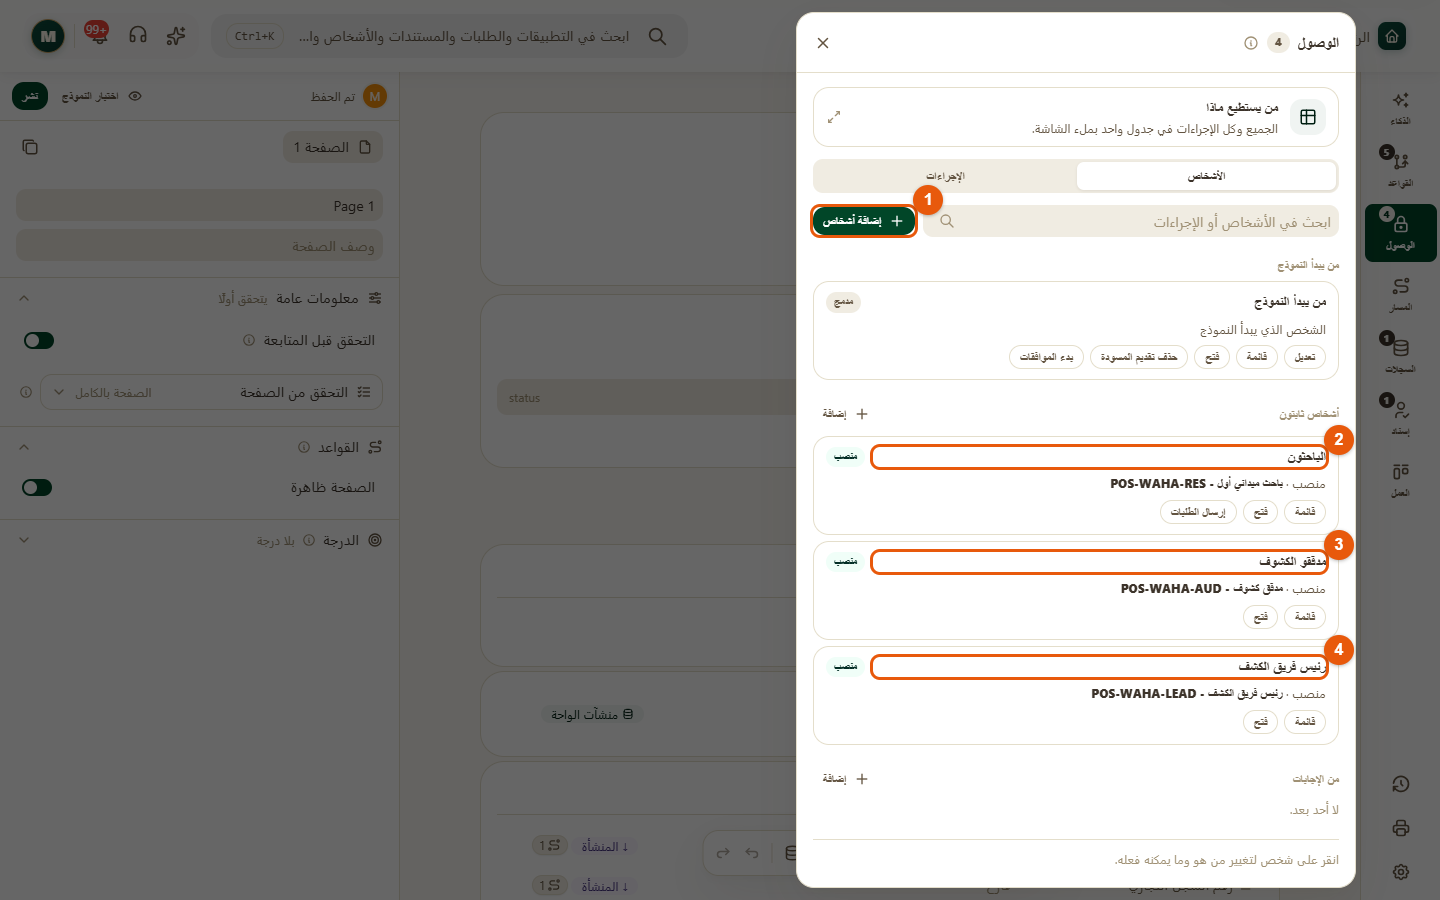
\includegraphics[width=0.85\linewidth]{assets/screens/b-access.png}
\caption{الوصول إلى النموذج}
\label{fig:build-access}
\shotnote{صورة توضيحية من التنفيذ السابق؛ اتبع العلامات المرقّمة، واستخدم أسماء منظمتك وقيمها الواردة في النص بدلاً من بيانات الصورة. كل بطاقة دور للنموذج، مسنَد إلى منصب، وتحته إجراءاته. ① «إضافة أشخاص». ② الباحثون. ③ المدققون. ④ رئيس الفريق.}
\end{figure}

\subsection{خطوات التنفيذ والحفظ}
إذا كان العنصر موجوداً، افتحه وتابع من خطوة الإعداد التالية بدلاً من إنشاء نسخة مكررة. توضح الخطوات أيضاً طريقة إنشائه عند الحاجة؛ وجوده مسبقاً لا يلغي شرح طريقة بنائه.

\begin{enumerate}
\item افتح «الوصول» ← «إضافة» بجانب «أشخاص ثابتون». اكتب الاسم، واختر المنصب في «من»، وحدّد الإجراءات، ثم اضغط «حفظ في المسودة».
\item افتح «إسناد»، وفعّل «يمكن التكليف به».
\item اضغط «نشر»، وراجع التغييرات، ثم اضغط «نشر».
\end{enumerate}

\textbf{تحقق:} يجب أن تعمل الصلاحيات المقصودة في النسخة المنشورة. إذا كان النموذج غير متاح عند التكليف، راجع التكليف والوصول والنشر قبل إنشاء بديل.

\section{أعدّ خطة التكليف وأطلقها}
\label{sec:build-plan}

الخطة تربط النموذج بالسجلات والمرشحين. لا يفترض هذا الفصل وجود خطة باسم معين؛ افتح الخطة المرتبطة بالنموذج إن كانت موجودة، وحافظ على اسمها وإعدادها.

\begin{rcnote}[من منظمتك: حماية المستهلك]
إذا كانت الخطة تستهدف «فرن الأمانة» وتُسند إلى «باحث ميداني — 01»، فطابق المرشح مع «نور حسن — تجريبي» وتعيينه النشط. هذا معيار للتحقق من المعاينة، وليس ادعاءً بوجود تكليف أُطلق بالفعل.
\end{rcnote}

\begin{figure}[H]
\centering
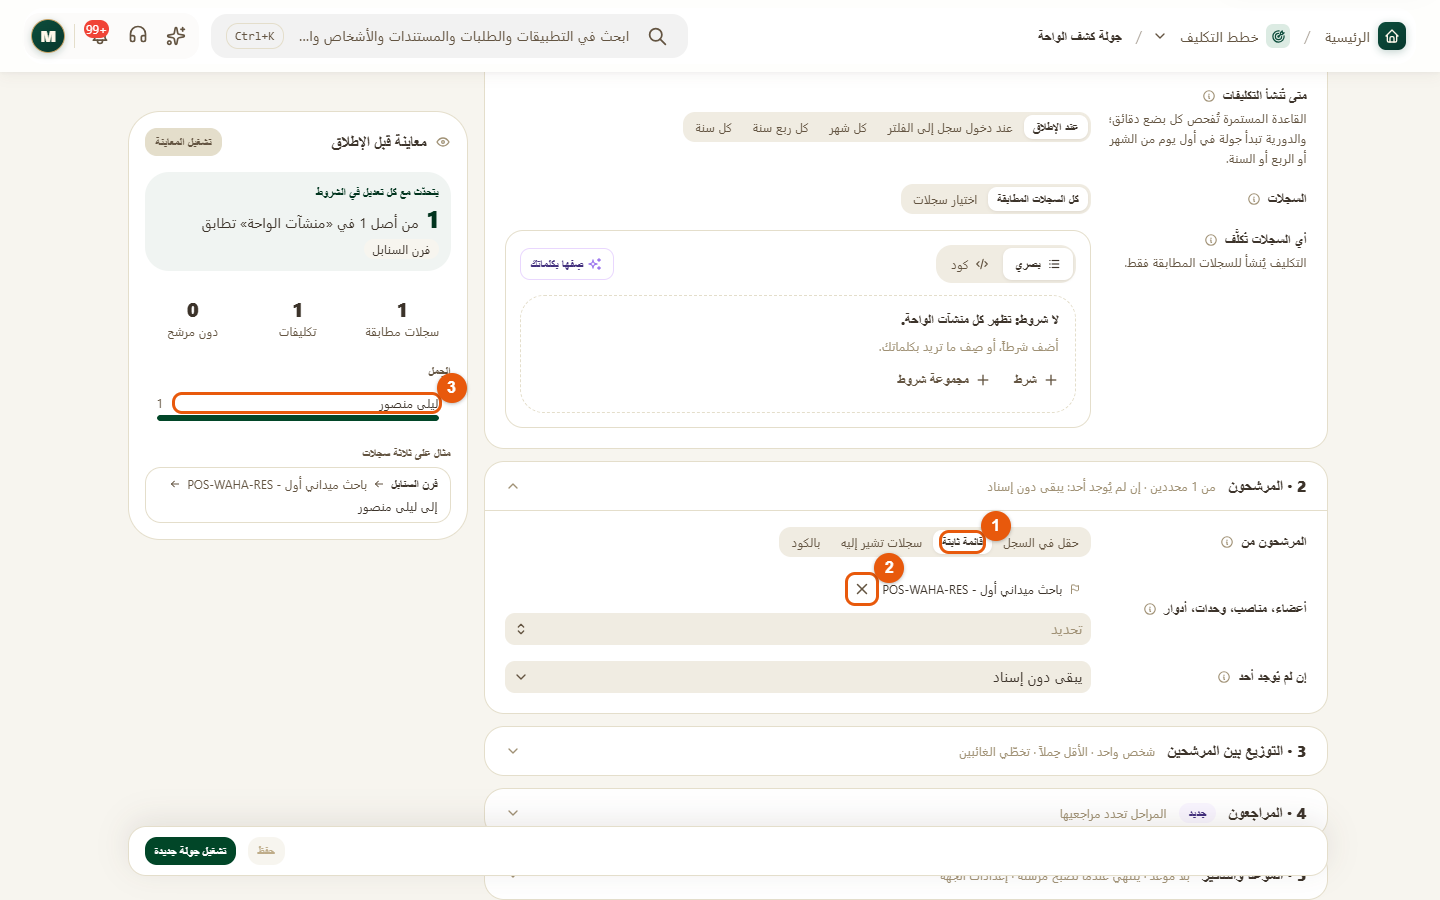
\includegraphics[width=0.95\linewidth]{assets/screens/b-plan.png}
\caption{المرشحون ومعاينة الخطة}
\label{fig:build-plan}
\shotnote{صورة توضيحية من التنفيذ السابق؛ اتبع العلامات المرقّمة، واستخدم أسماء منظمتك وقيمها الواردة في النص بدلاً من بيانات الصورة. تحسب المعاينة كل تكليف قبل إنشائه. وإذا ظهر سجل «دون مرشح»، فراجع التعيين أو المنصب. ① «قائمة ثابتة». ② المنصب المرشَّح. ③ الشخص الذي سيصله التكليف.}
\end{figure}

\subsection{خطوات التنفيذ والحفظ}
إذا كان العنصر موجوداً، افتحه وتابع من خطوة الإعداد التالية بدلاً من إنشاء نسخة مكررة. توضح الخطوات أيضاً طريقة إنشائه عند الحاجة؛ وجوده مسبقاً لا يلغي شرح طريقة بنائه.

اختر النموذج «كشف منشأة تجارية لطلب سجل تجاري»، والمنصب «باحث ميداني — 01». عند استخدام «فرن الأمانة» في المعاينة، تحقق من ظهور «نور حسن — تجريبي» مرشحاً. احتفظ باسم الخطة الموجود؛ لم تُطابق أسماء الخطط في هذه المراجعة.

\begin{enumerate}
\item افتح «خطط التكليف» ← «خطة جديدة»، واختر النموذج، واكتب «اسم الخطة»، ثم اضغط «إنشاء والإعداد». وإذا ظهر «التكليف متوقف لهذا النموذج»، فاضغط «تشغيل التكليف».
\item افتح «2 · المرشحون»، واختر «قائمة ثابتة»، ثم أضف المنصب.
\item اضغط «تشغيل المعاينة»، ثم «حفظ»، ثم «إنشاء التكليفات».
\end{enumerate}

\textbf{تحقق:} إذا ظهر سجل «دون مرشح»، فراجع قواعد الاختيار والتعيين. إذا لم توجد خطة، فهذه الخطوة غير معدّة بعد؛ وجود النموذج لا يعني وجود خطة، ولا يلزم إنشاء واحدة لتكملة القراءة.

\section{شغّل الكشف بحساب الباحث}
\label{sec:build-run-researcher}

يعمل الباحث بحسابه المخوّل وعلى التكليف الموجه إليه. فتح الصفحة الرئيسية وحده لا يثبت وصول التكليف أو نجاح الإرسال.

\begin{rcnote}[من منظمتك: حماية المستهلك]
العضو المقصود هو «نور حسن — تجريبي» برقم \en{DEMO-CP-002}. عندما يصله تكليف على «فرن الأمانة»، يطابق المنشأة والنموذج قبل إدخال نتيجة الكشف الفعلية؛ لا يستخدم عنواناً أو توصية مفترضة من الدليل.
\end{rcnote}

\begin{figure}[H]
\centering
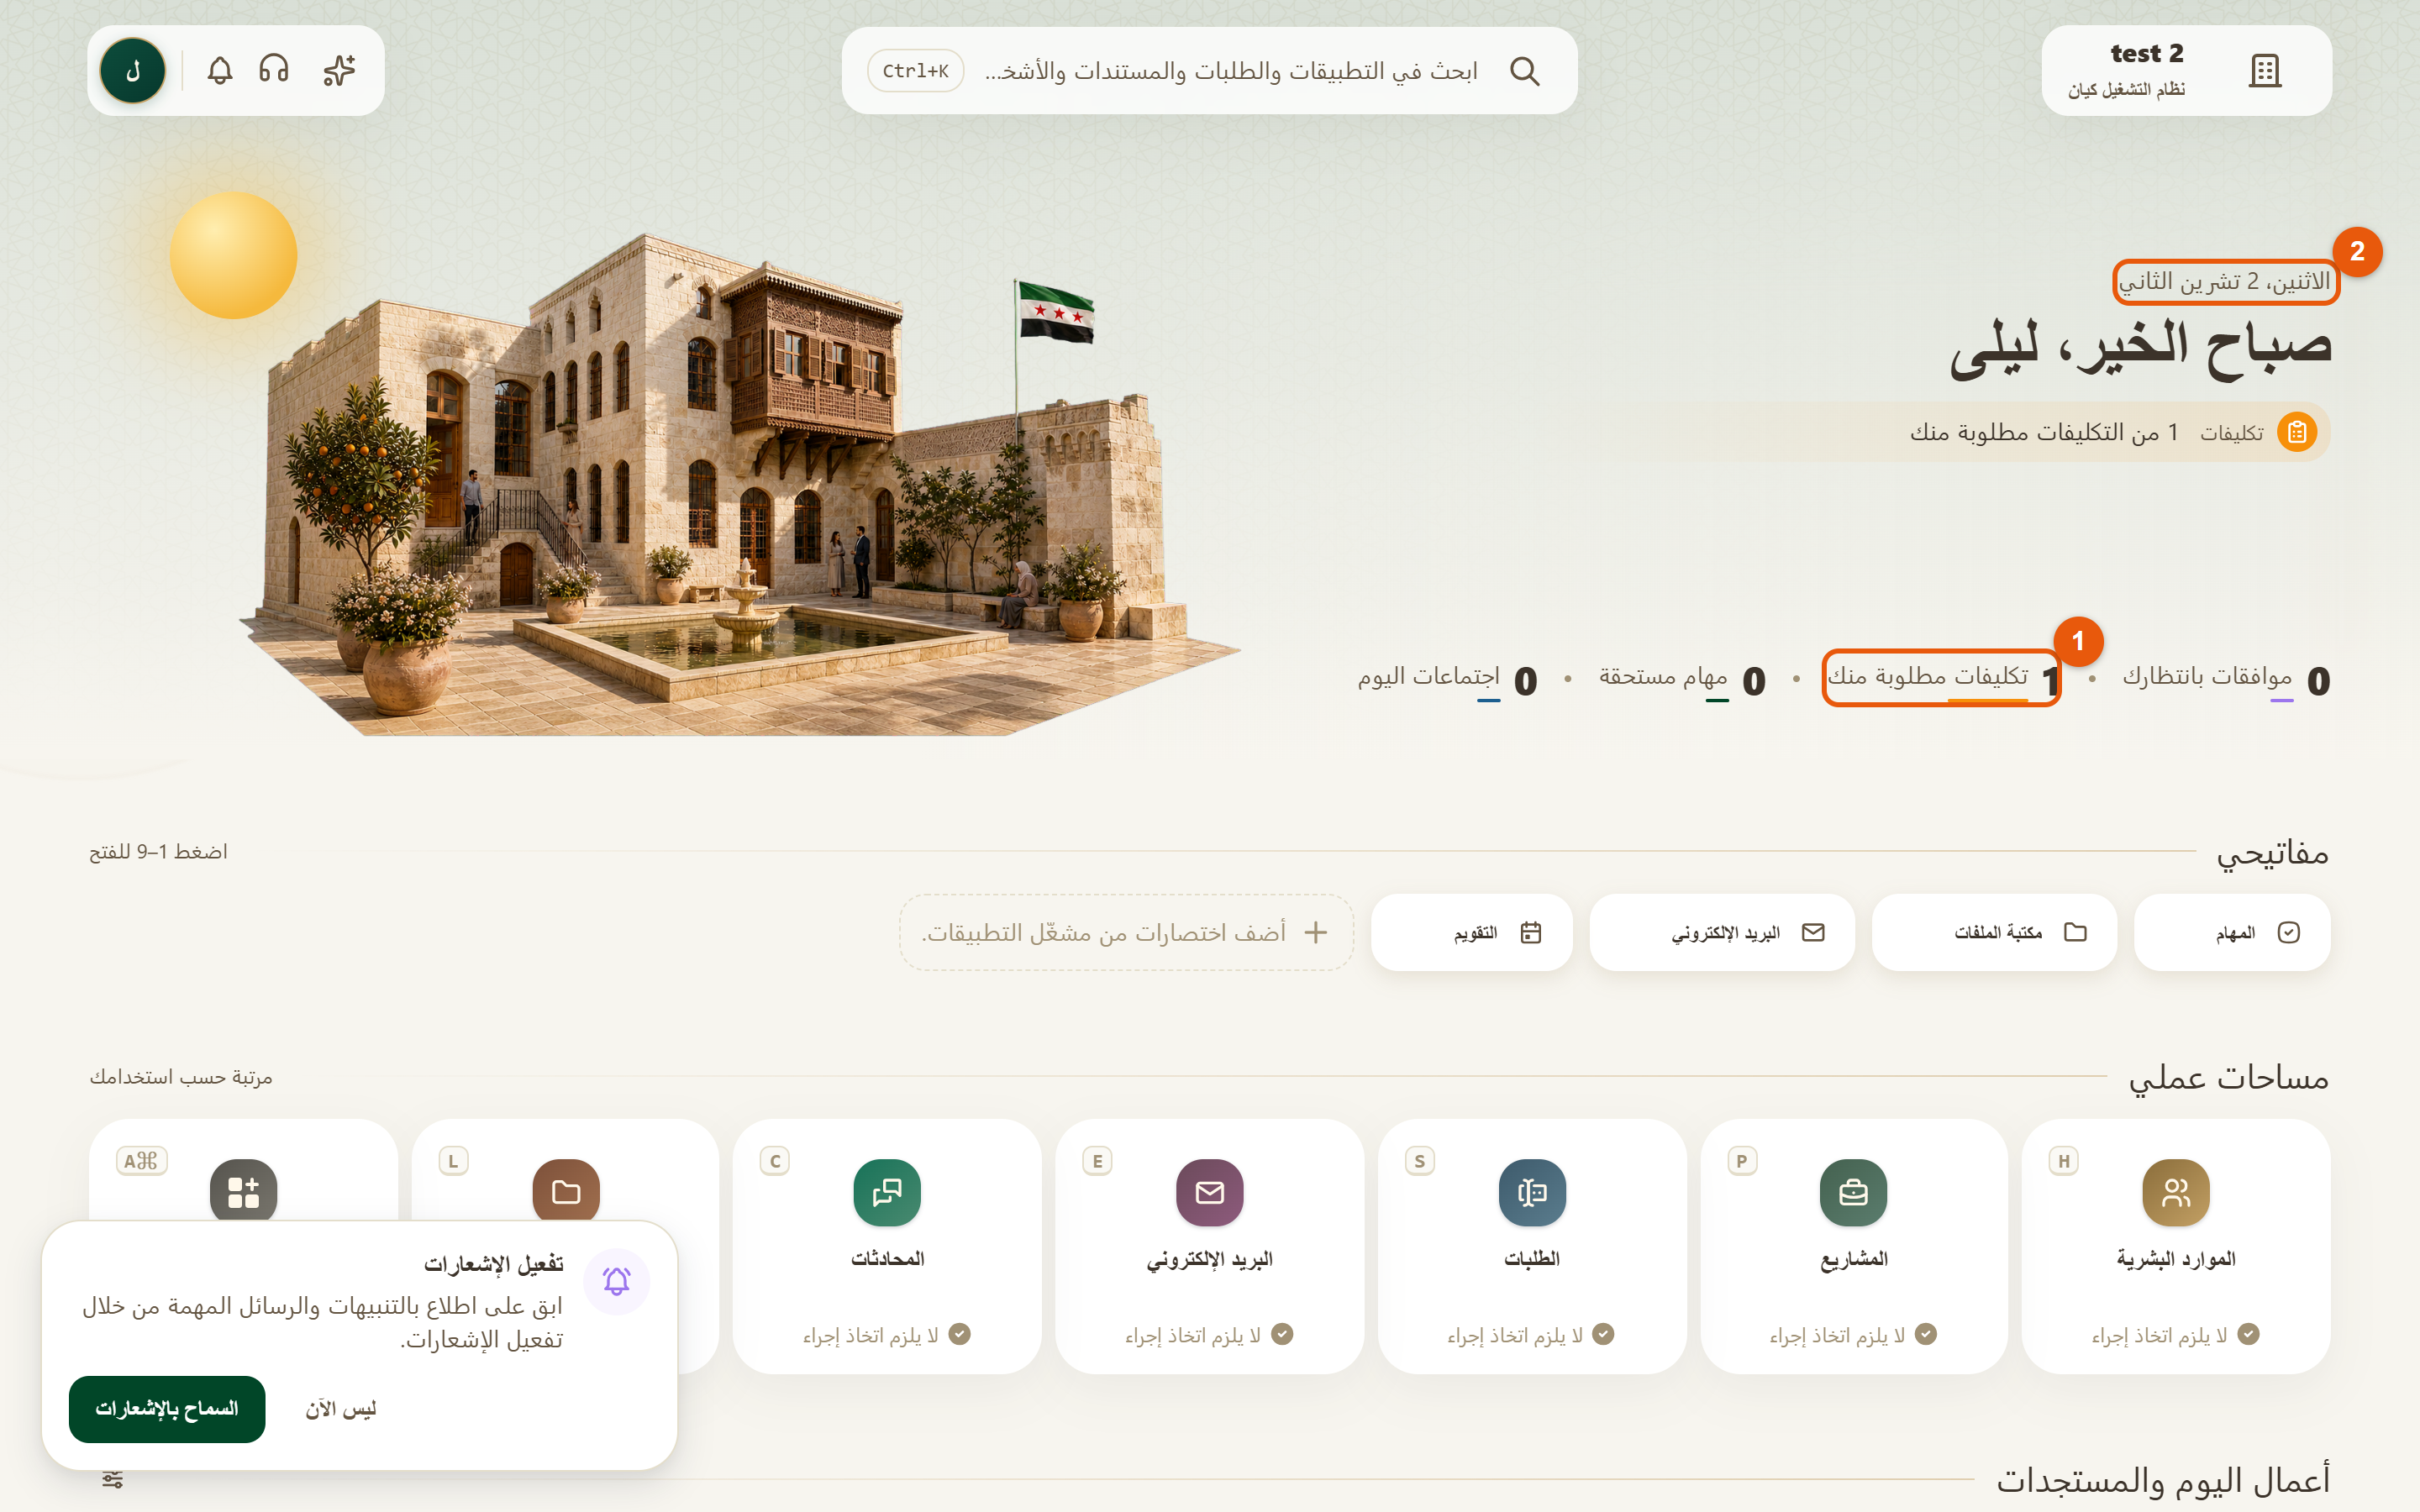
\includegraphics[width=0.95\linewidth]{assets/screens/b-laila-home.png}
\caption{الصفحة الرئيسية للباحث}
\label{fig:build-laila-home}
\shotnote{صورة توضيحية من التنفيذ السابق؛ اتبع العلامات المرقّمة، واستخدم أسماء منظمتك وقيمها الواردة في النص بدلاً من بيانات الصورة. تجمع الصفحة الرئيسية ما ينتظر الموظف، ويظهر التاريخ بالأشهر الشامية. ① «تكليفات مطلوبة منك». ② التاريخ.}
\end{figure}

\begin{figure}[H]
\centering
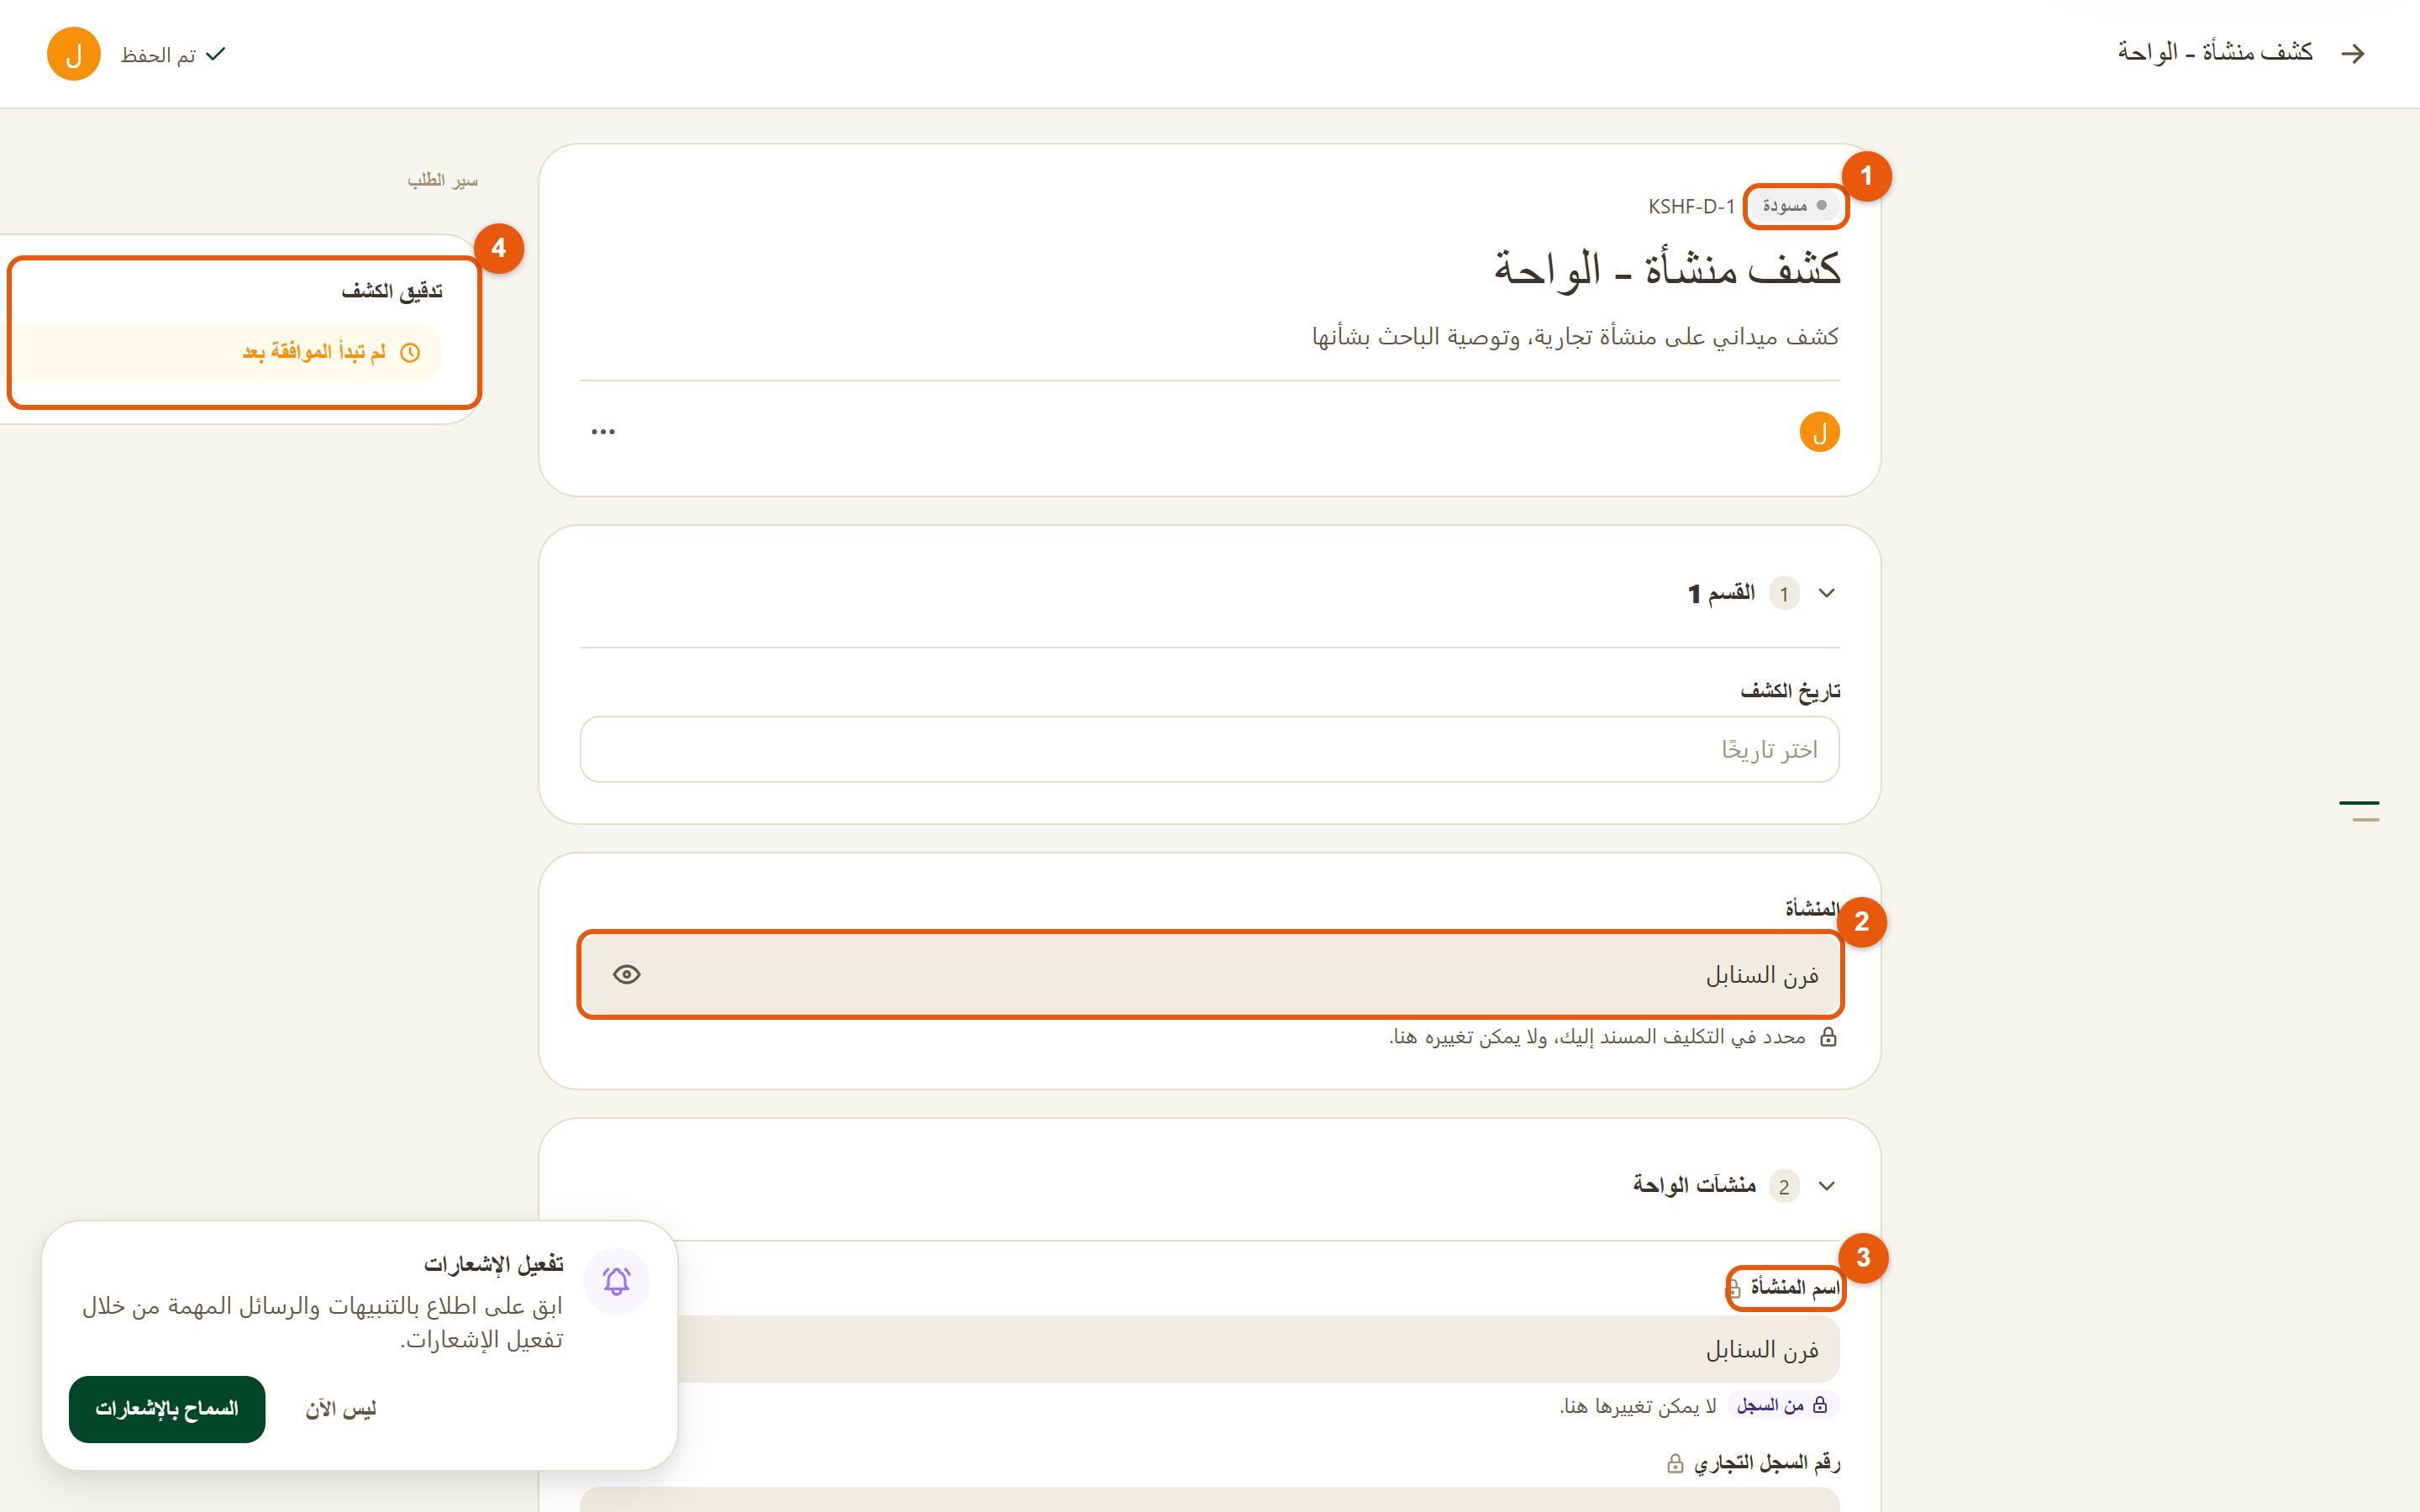
\includegraphics[width=0.95\linewidth]{assets/screens/b-laila-form.png}
\caption{الكشف كما يفتحه الباحث}
\label{fig:build-laila-form}
\shotnote{صورة توضيحية من التنفيذ السابق؛ اتبع العلامات المرقّمة، واستخدم أسماء منظمتك وقيمها الواردة في النص بدلاً من بيانات الصورة. تأتي المنشأة من التكليف ولا يغيّرها الباحث. وتأتي بياناتها من سجلها، فيُقفل ما يُقرأ فقط. ① الحالة: «مسودة» حتى الإرسال. ② المنشأة: «محدد في التكليف المسند إليك». ③ حقل مقفل «من السجل». ④ «تدقيق الكشف» في انتظار الإرسال.}
\end{figure}

\subsection{خطوات التنفيذ والحفظ}
إذا كان العنصر موجوداً، افتحه وتابع من خطوة الإعداد التالية بدلاً من إنشاء نسخة مكررة. توضح الخطوات أيضاً طريقة إنشائه عند الحاجة؛ وجوده مسبقاً لا يلغي شرح طريقة بنائه.

\begin{enumerate}
\item اضغط «تكليفات مطلوبة منك»، ثم «ابدأ» بجانب المنشأة.
\item املأ الأسئلة. وإذا عدّلت حقلاً من السجل، يظهر تحته النص القديم مع «استعادة».
\item اضغط «إرسال الطلب»، ثم أكّد.
\end{enumerate}

\textbf{تحقق:} راجع رقم الكشف وحالته بعد الإرسال، ولا تفترض رقماً أو عدداً ثابتاً للتكليفات. إذا لم يصل التكليف، ارجع إلى الخطة والمرشحين والصلاحيات قبل إعادة الإرسال.

\section{قرّر بحساب المدقق}
\label{sec:build-run-reviewer}

قرار المدقق يخص الكشف الذي وصل إليه. ونجاح القرار لا يثبت وحده أن سجل المنشأة تحدّث؛ يجب فحص نتيجة الربط إذا كان النموذج يكتب إلى السجلات.

\begin{rcnote}[من منظمتك: حماية المستهلك]
العضو المقصود هو «ريم خالد — تجريبي» برقم \en{DEMO-CP-003}، وشاغلة منصب «مدقق كشوف المنشآت — 01». تراجع الكشف الذي أرسله نور وتستخدم الخيارات الظاهرة في خطوة الموافقة الحالية.
\end{rcnote}

\begin{figure}[H]
\centering
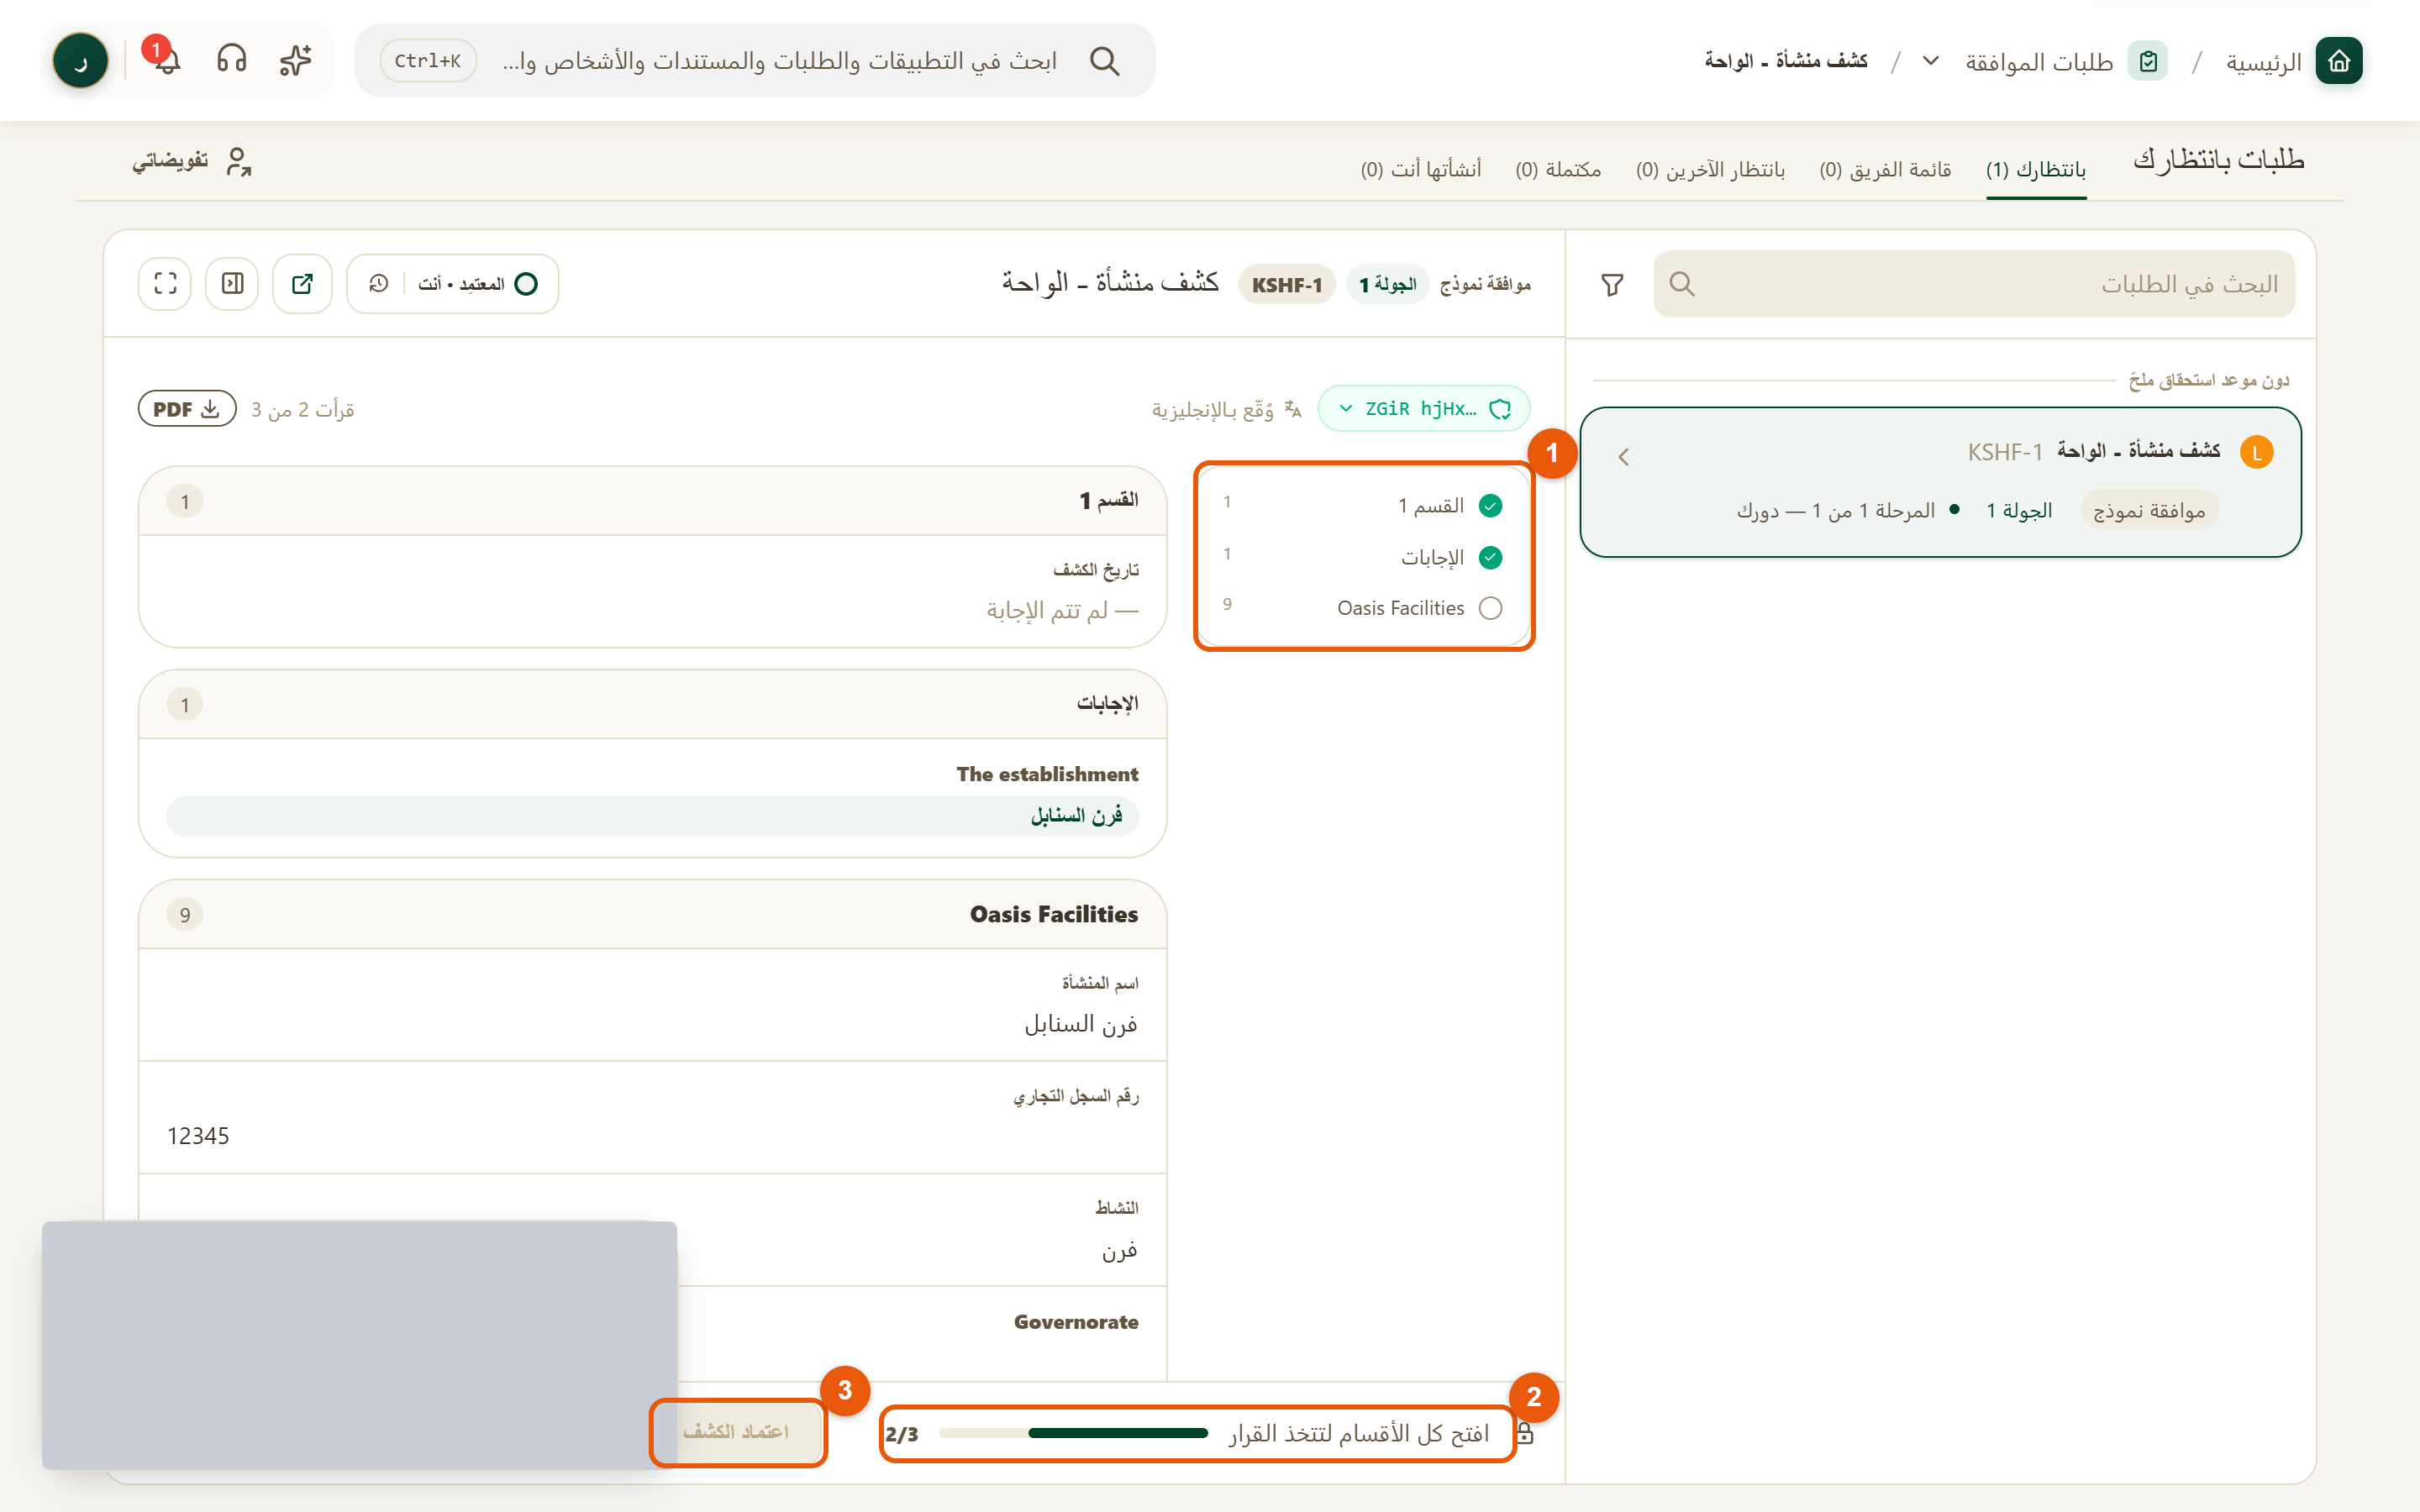
\includegraphics[width=0.95\linewidth]{assets/screens/b-decide.png}
\caption{شاشة قرار المدقق}
\label{fig:build-decide}
\shotnote{صورة توضيحية من التنفيذ السابق؛ اتبع العلامات المرقّمة، واستخدم أسماء منظمتك وقيمها الواردة في النص بدلاً من بيانات الصورة. تعدّ الشاشة الأقسام المقروءة، ولا تفتح القرار قبل اكتمالها. ① الأقسام وما قُرئ منها. ② «افتح كل الأقسام لتتخذ القرار». ③ أزرار القرار.}
\end{figure}

\begin{figure}[H]
\centering
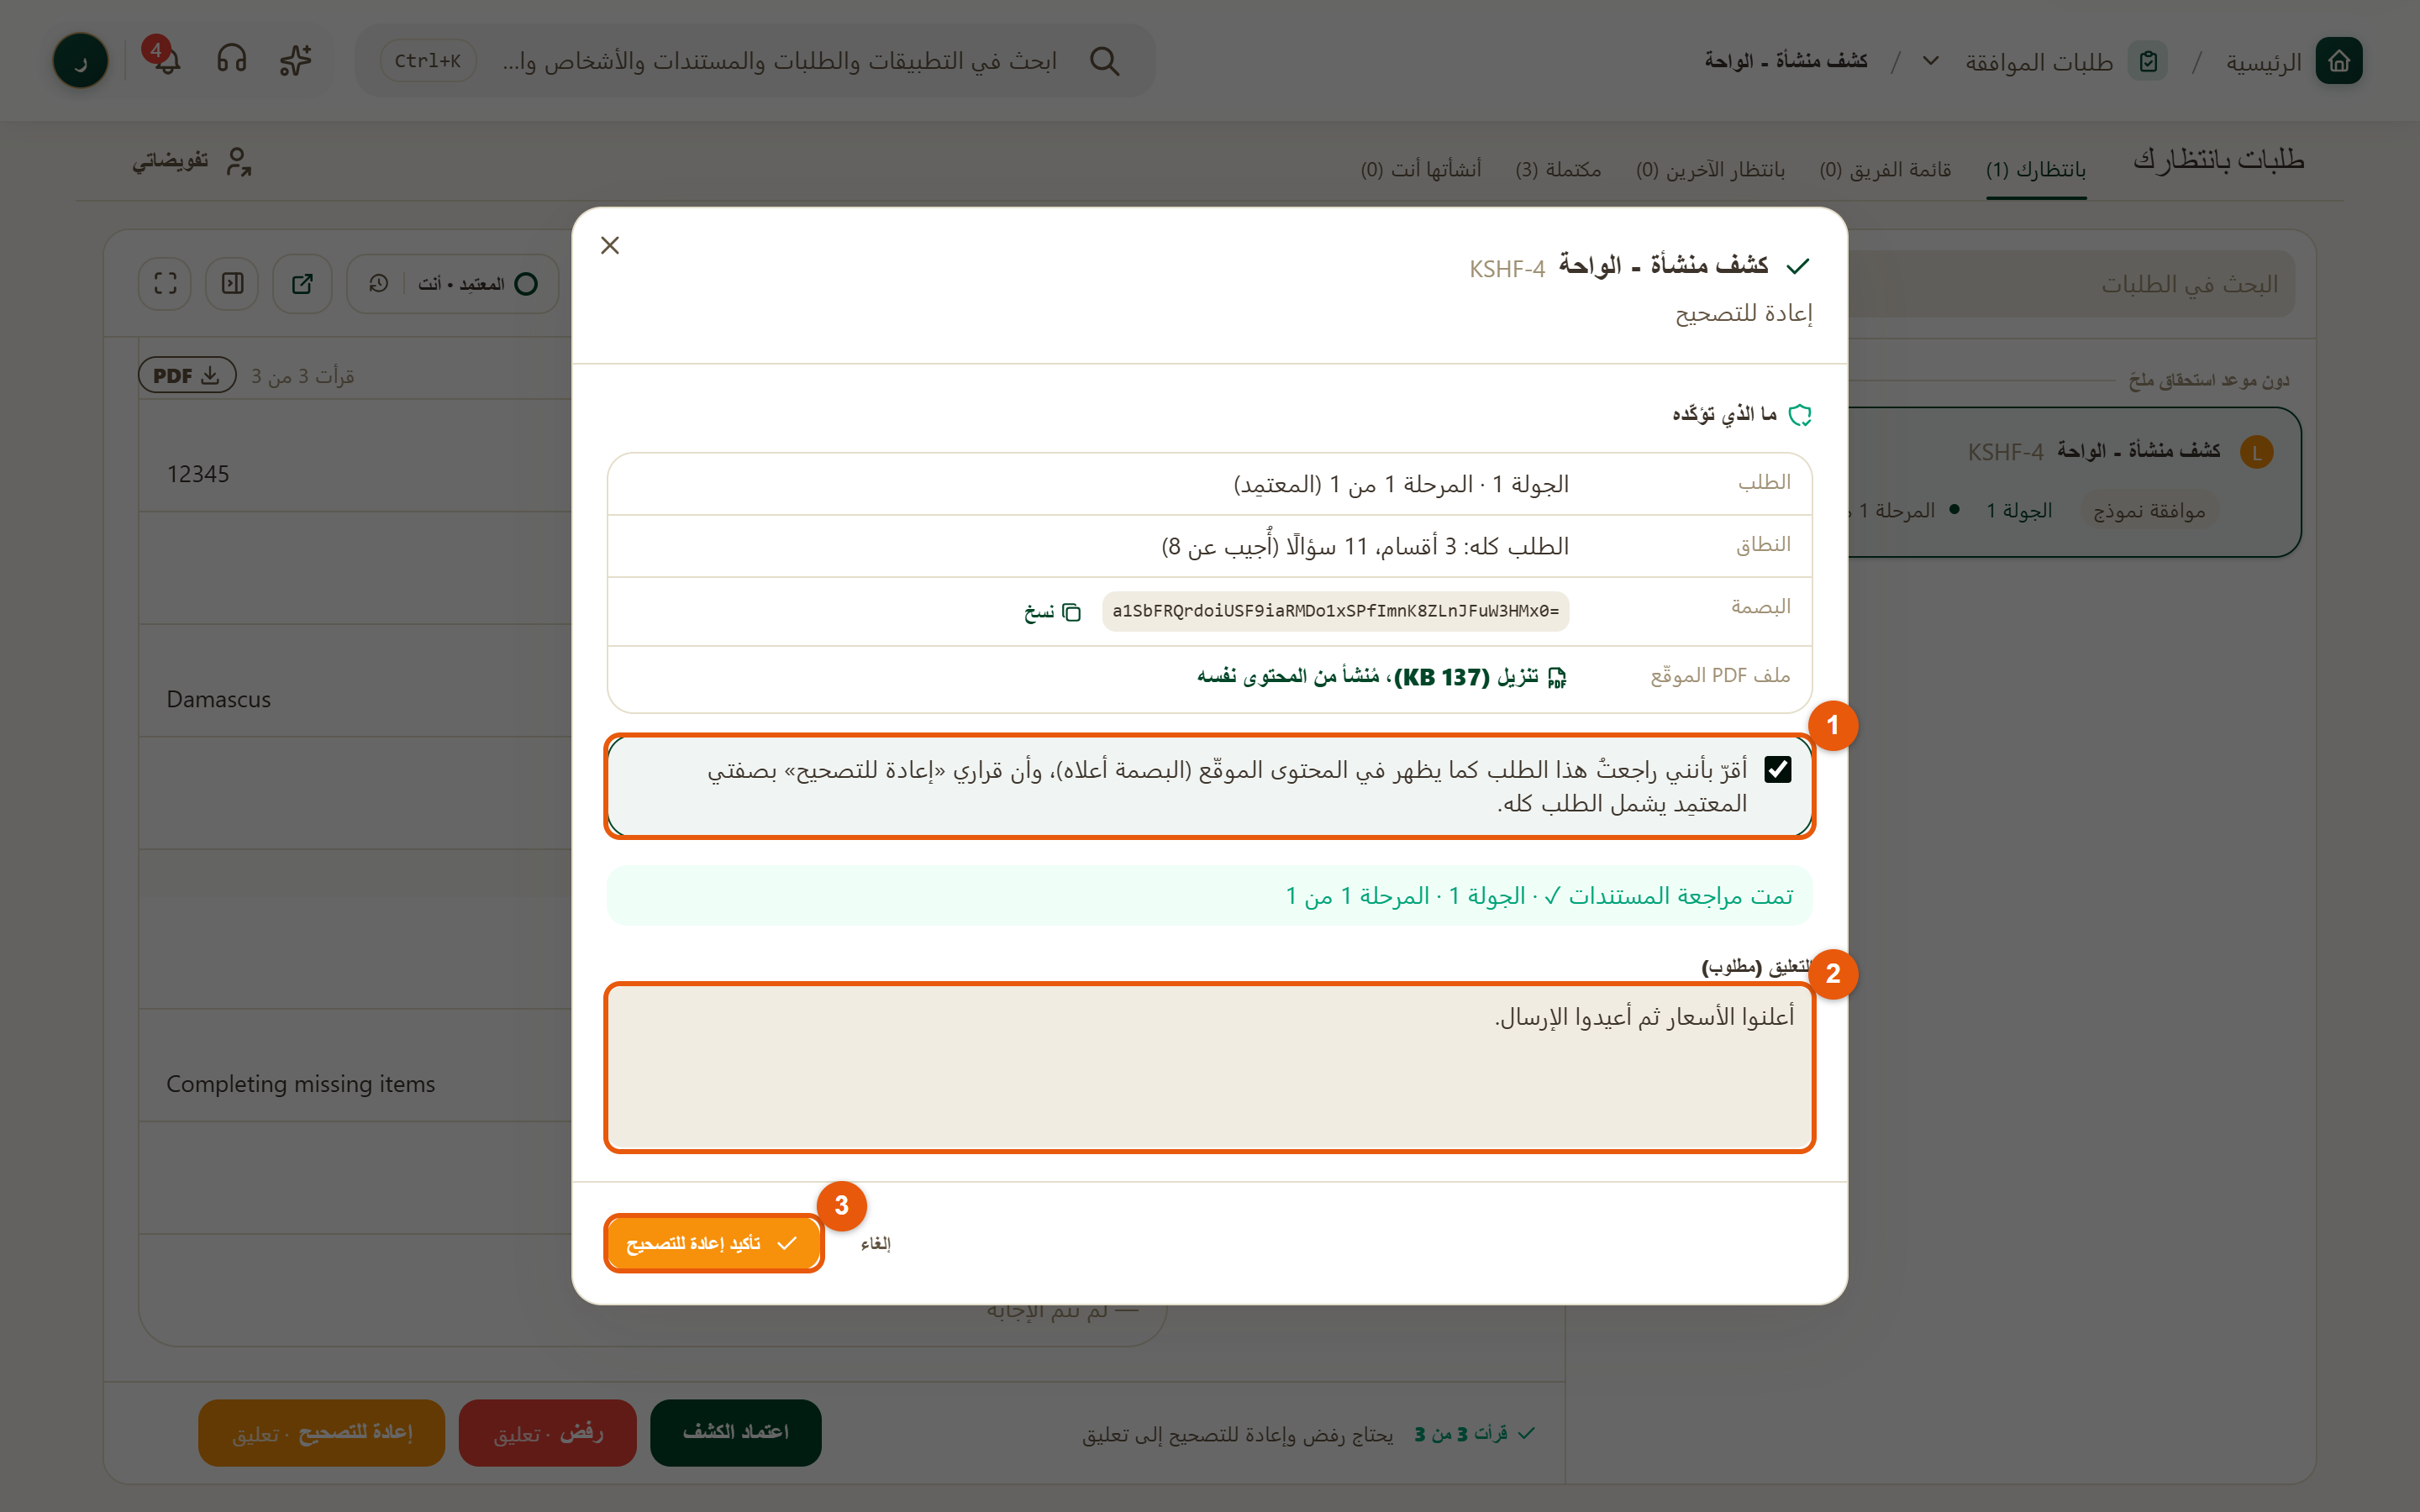
\includegraphics[width=0.95\linewidth]{assets/screens/b-return-dlg.png}
\caption{تأكيد القرار}
\label{fig:build-return-dlg}
\shotnote{صورة توضيحية من التنفيذ السابق؛ اتبع العلامات المرقّمة، واستخدم أسماء منظمتك وقيمها الواردة في النص بدلاً من بيانات الصورة. يلخّص التأكيد ما يقرّ به المدقق، ومعه بصمة المحتوى وملف PDF موقّع. ① الإقرار: لا يُقبل القرار دونه. ② «التعليق (مطلوب)» للرفض والإعادة. ③ زر التأكيد.}
\end{figure}

\begin{figure}[H]
\centering
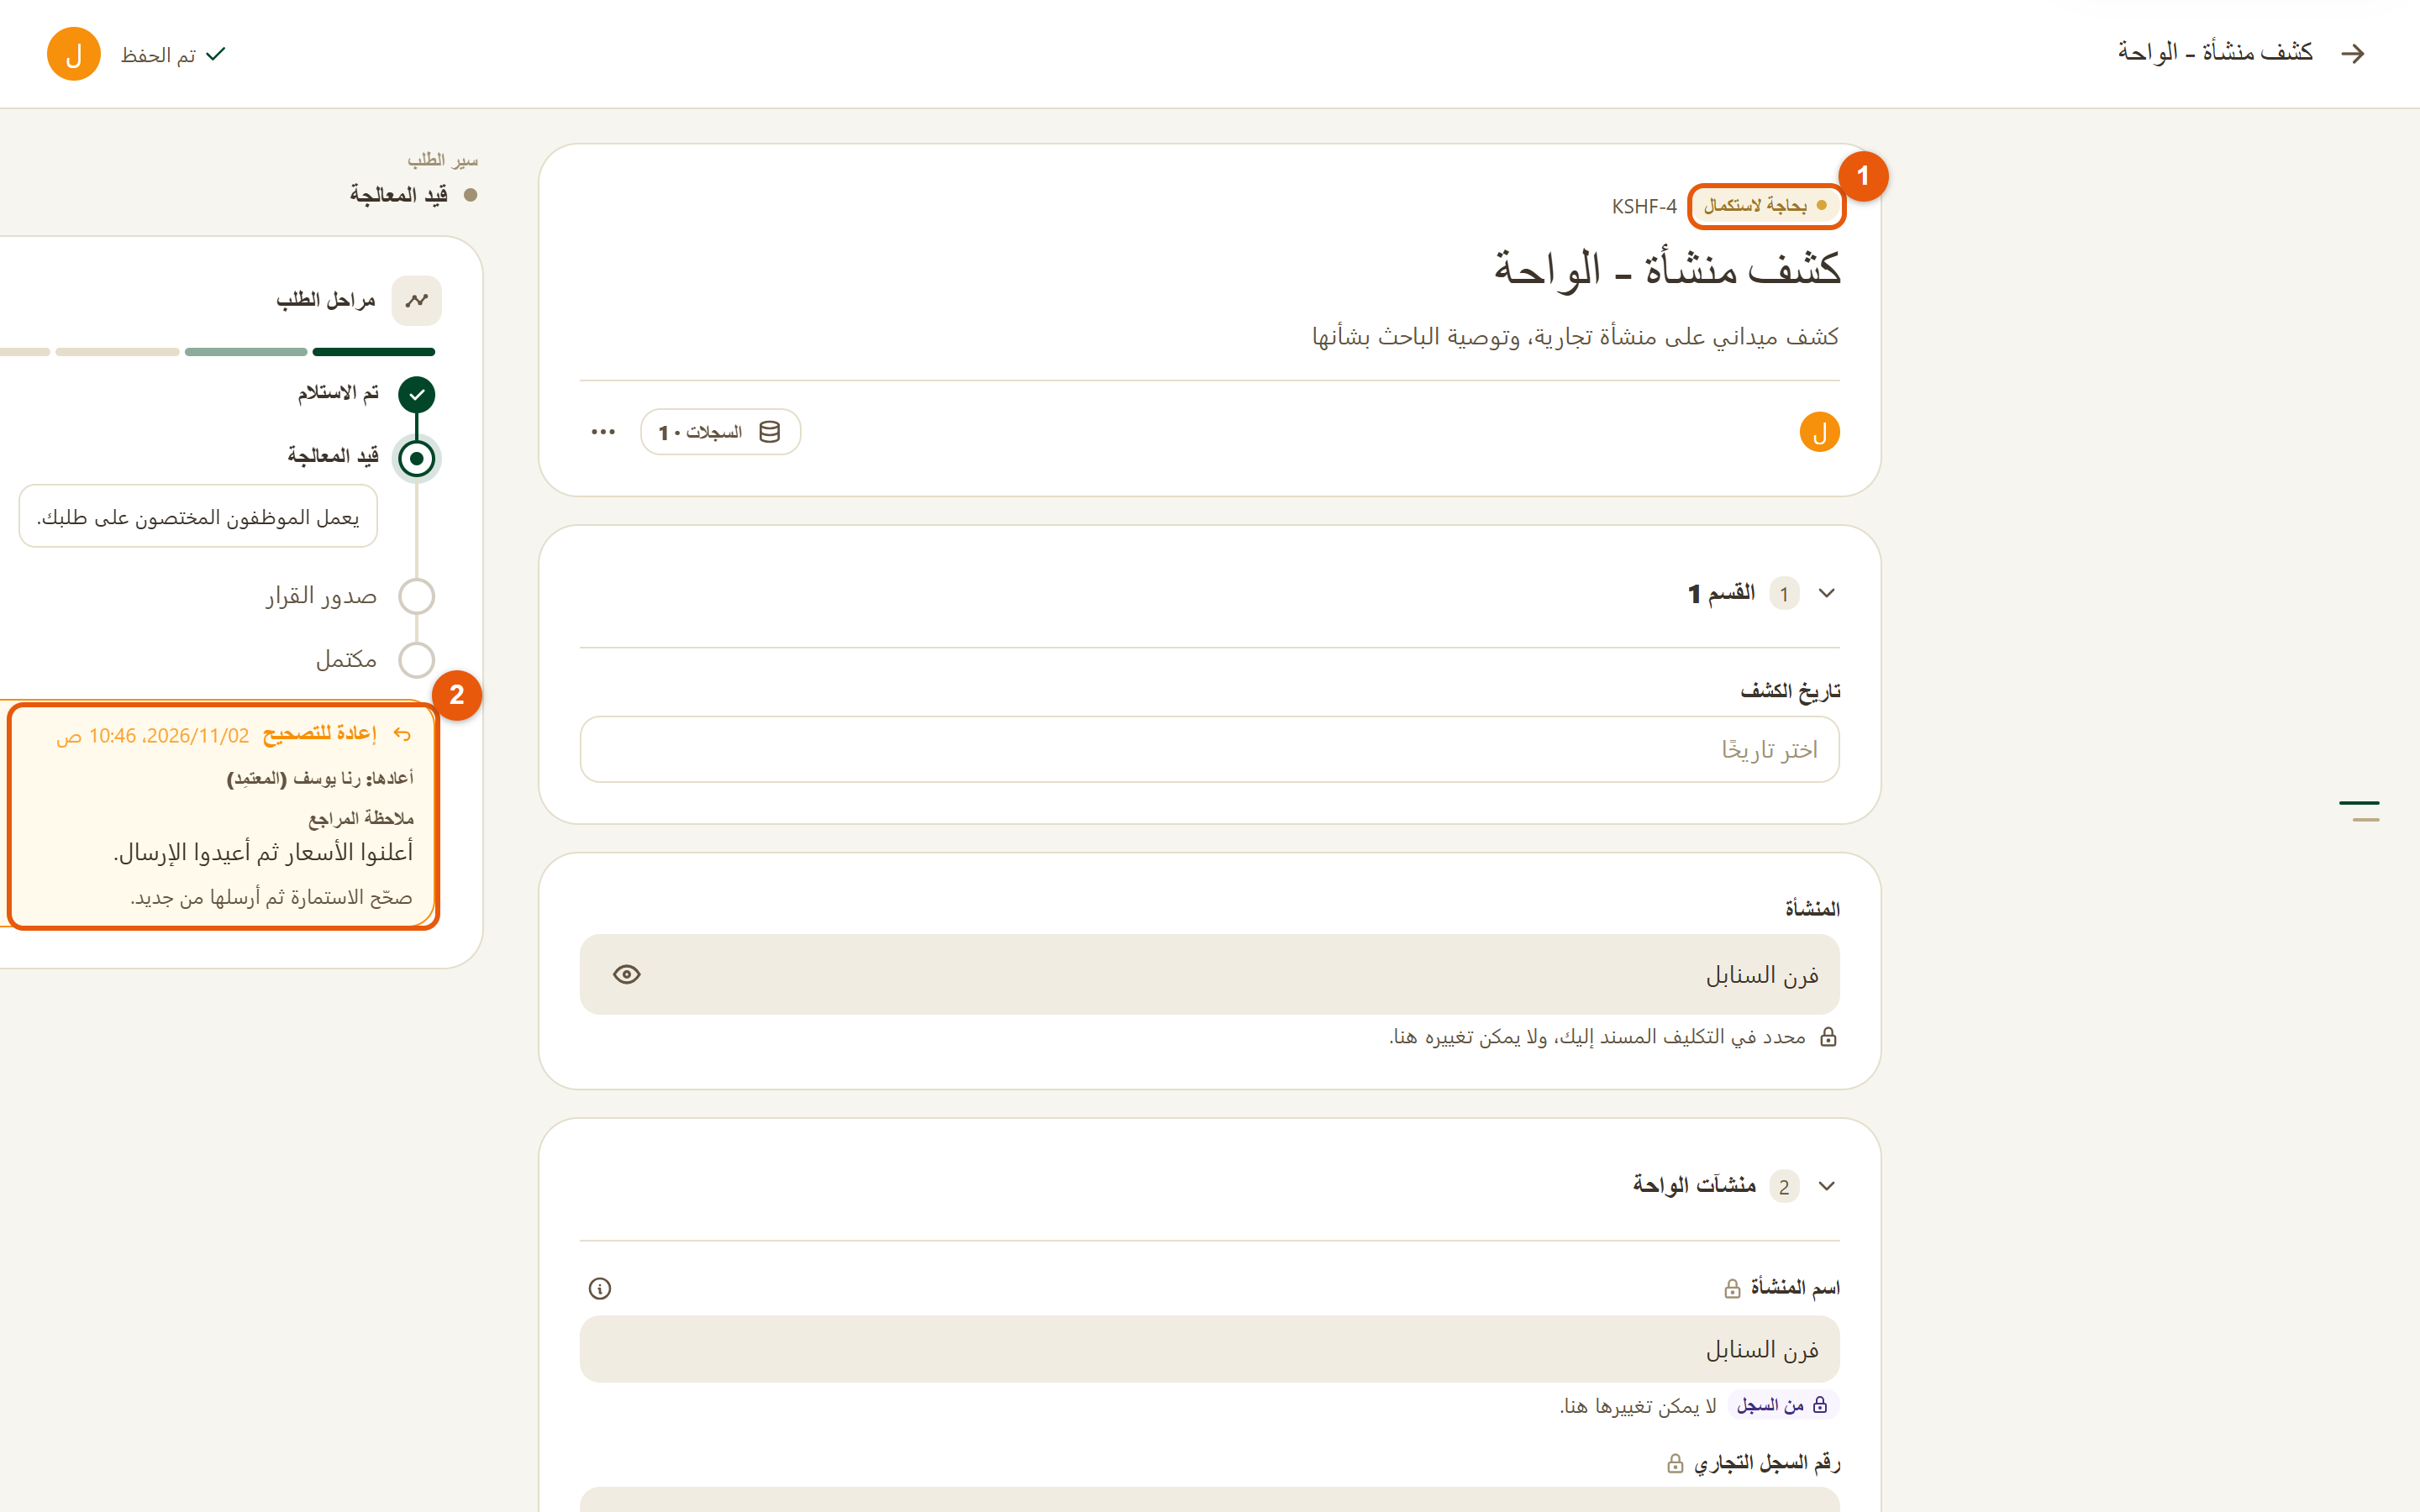
\includegraphics[width=0.95\linewidth]{assets/screens/b-returned.png}
\caption{ما يراه الباحث بعد الإعادة}
\label{fig:build-returned}
\shotnote{صورة توضيحية من التنفيذ السابق؛ اتبع العلامات المرقّمة، واستخدم أسماء منظمتك وقيمها الواردة في النص بدلاً من بيانات الصورة. يعود الكشف قابلاً للتعديل، ومعه ملاحظة المدقق. وإعادة إرساله تبدأ جولة موافقة جديدة. ① «بحاجة لاستكمال». ② «إعادة للتصحيح» مع اسم المدقق وملاحظته.}
\end{figure}

\begin{figure}[H]
\centering
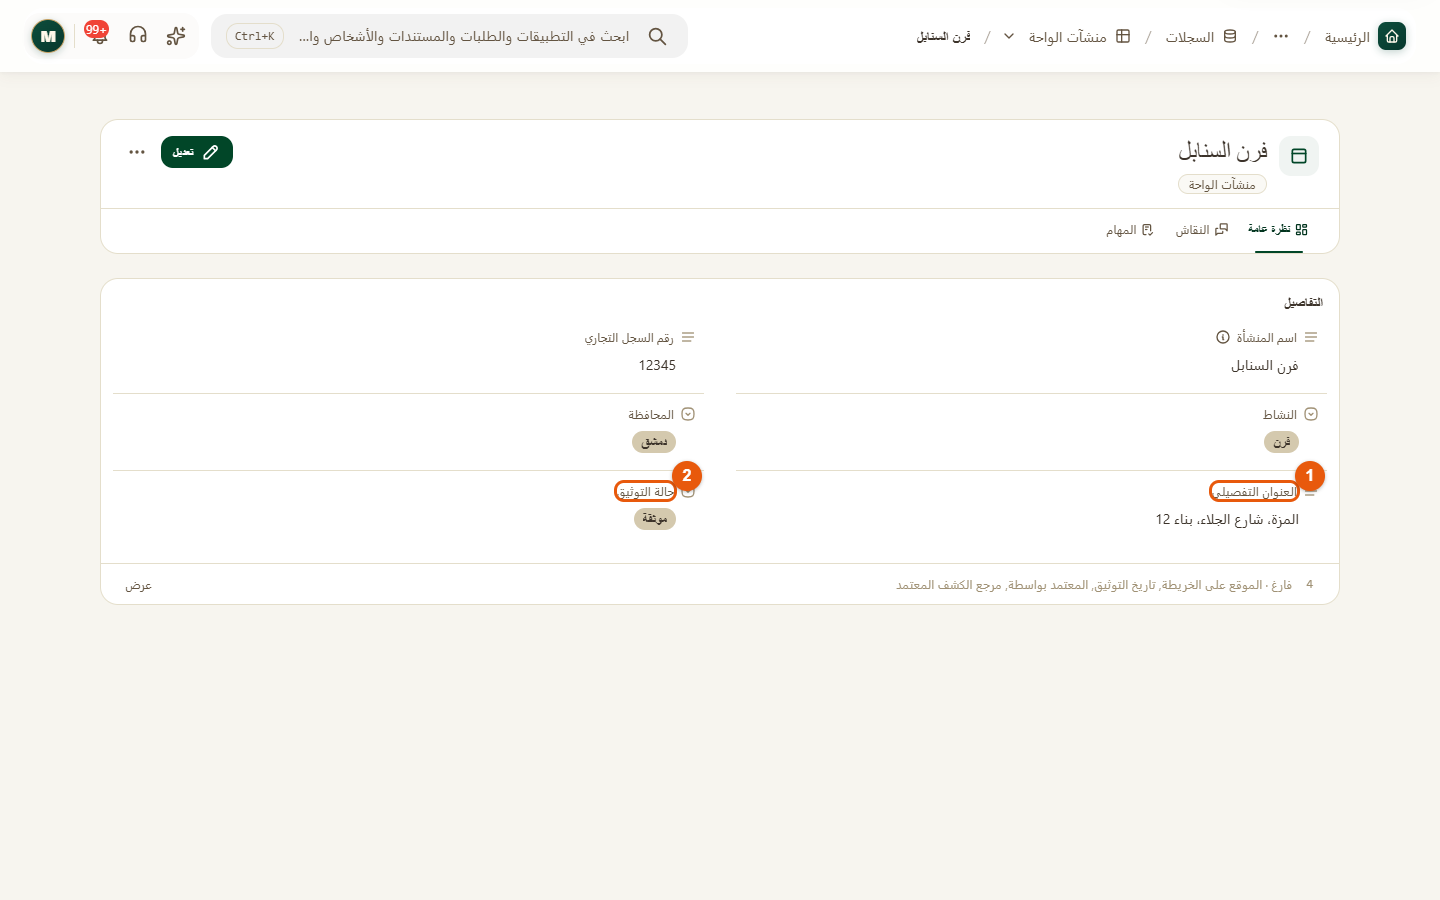
\includegraphics[width=0.95\linewidth]{assets/screens/b-record-after.png}
\caption{المنشأة بعد الاعتماد}
\label{fig:build-record-after}
\shotnote{صورة توضيحية من التنفيذ السابق؛ اتبع العلامات المرقّمة، واستخدم أسماء منظمتك وقيمها الواردة في النص بدلاً من بيانات الصورة. توضح الصورة نتيجة الكتابة بعد الاعتماد في التنفيذ السابق، وليست إثباتاً لتحديث منشأة في منظمتك. ① «العنوان التفصيلي» الجديد. ② «حالة التوثيق»: «موثقة».}
\end{figure}

\subsection{خطوات التنفيذ والحفظ}
إذا كان العنصر موجوداً، افتحه وتابع من خطوة الإعداد التالية بدلاً من إنشاء نسخة مكررة. توضح الخطوات أيضاً طريقة إنشائه عند الحاجة؛ وجوده مسبقاً لا يلغي شرح طريقة بنائه.

\begin{enumerate}
\item افتح «موافقات بانتظارك»، ثم الكشف.
\item افتح كل قسم من القائمة الجانبية، ومرّر حتى نهايته، حتى يكتمل عدّاد قراءة الأقسام الموجودة في الكشف.
\item اضغط القرار، واكتب التعليق إن طُلب، وحدّد الإقرار، ثم اضغط «تأكيد».
\end{enumerate}

\textbf{تحقق:} ميّز بين اكتمال قرار الموافقة ونجاح تحديث المنشأة. إذا كانت الأزرار معطلة، راجع متطلبات القراءة والتعليق والصلاحية؛ وإذا فشلت الكتابة، راجع السبب قبل تكرار العملية.

\section{اضبط لوحة المؤشرات خطوة بخطوة}
\label{sec:build-dashboard}

لوحة المعلومات تعرض بيانات مصدرها السجلات والصلاحيات والتصفية. لم تُثبت هذه المراجعة اسم لوحة خاصة بالكشف أو أرقامها، ولذلك لا يضع الفصل لوحة أو منشآت صناعية أو نتائج رقمية مفترضة ضمن محتوى المنظمة.

\begin{rcnote}[من منظمتك: حماية المستهلك]
المصدر الذي طابقنا اسمه هو «المنشآت التجارية». ظهرت في قراءة الأسماء ثلاثة سجلات: «فرن الأمانة» و«مطعم الياسمين» و«سوبر ماركنت النور». هذه لقطة وقت المراجعة، وليست قيمة مفروضة على أي لوحة أو حساب آخر.
\end{rcnote}

\begin{enumerate}
\item افتح «لوحات المعلومات» وابحث عن لوحة مرتبطة بالعمل الحالي إن وُجدت.
\item راجع مصدر كل عنصر واسمه والتصفية والصلاحيات، قبل مقارنة الرقم بقائمة السجلات نفسها.
\item استخدم الحقول الموجودة فقط. لا تفترض وجود «عدد العمال» أو «الطاقة الإنتاجية بالطن» أو «حالة الترخيص» في النوع.
\end{enumerate}

\textbf{تحقق:} قارن العنصر بقائمته تحت الحساب والتصفية نفسيهما. إذا كانت اللوحة موجودة، افتح محررها وتابع الشرح التالي؛ وإذا احتجت إنشاء لوحة، توضح الخطوات طريقة إنشائها دون نسبتها إلى إعداد قائم لم نتحقق منه.

\subsection{خطوات بناء اللوحة بالصور المرقّمة}

الخطوات التالية تحفظ شرح أدوات اللوحة كاملاً. اختر نوع السجلات والحقول الموجودة في منظمتك؛ إذا كان مصدر المنشآت التجارية مناسباً فاستعمله، ولا تنشئ نوع «المنشآت الصناعية» لمجرد أنه ظاهر في صور التدريب. فقرة إنشاء النوع تشرح طريقة الإنشاء عند الحاجة فقط. أسماء اللوحات وخطط العمل تُؤخذ من إعدادك الحالي، ولا تفترض هذه الصور وجود لوحة بعينها.

\subsection{حدّد نوع السجلات الذي ستقرأ منه اللوحة}

\begin{figure}[H]
\centering
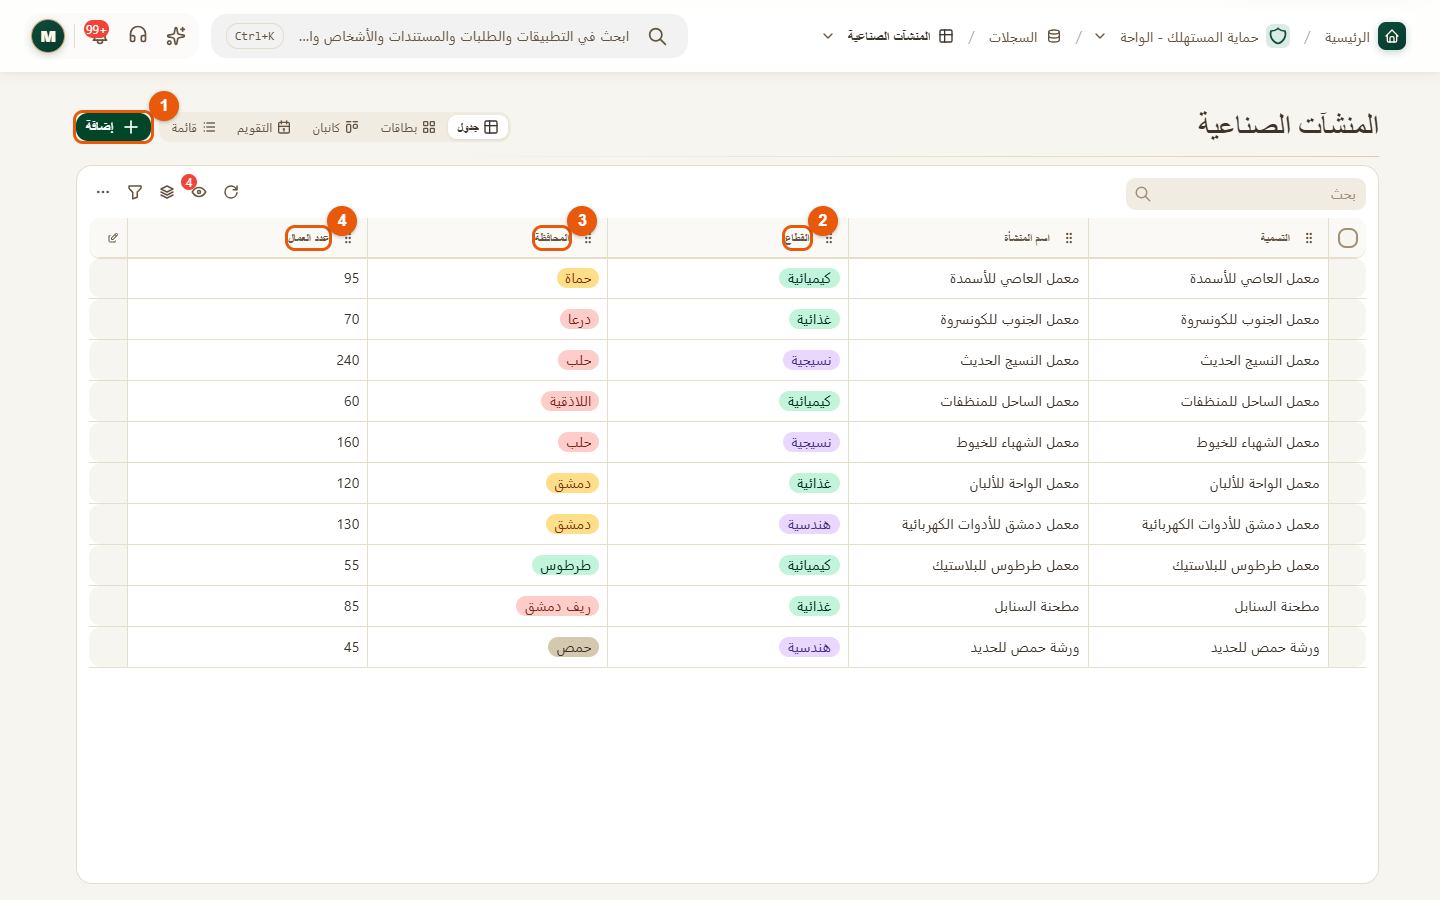
\includegraphics[width=0.95\linewidth]{assets/screens/i-records.png}
\caption{سجلات المنشآت الصناعية}
\label{fig:build-industrial-records}
\shotnote{صورة توضيحية من التنفيذ السابق؛ اتبع العلامات المرقّمة، واستخدم أسماء منظمتك وقيمها الواردة في النص بدلاً من بيانات الصورة. هذه البيانات التي ستقرؤها اللوحة، وتقابلها كل أرقامها. فإذا اختلف رقم في اللوحة عما تعدّه هنا يدوياً، فراجع إعداد العنصر. ① «إضافة»: يضيف منشأة. ② «القطاع». ③ «المحافظة». ④ «عدد العمال».}
\end{figure}

\begin{enumerate}
\item افتح «الكيانات»، ثم نوع السجلات الموجود الذي ستعرضه اللوحة، مثل «المنشآت التجارية»، وراجع حقوله المتاحة.
\item للعدّ استخدم عدد السجلات. وللمجموع اختر حقلاً رقمياً موجوداً، وللتوزيع اختر حقل التصنيف الموجود؛ لا تنقل أسماء الحقول الصناعية من الصورة إلى نوع آخر.
\item إذا كان العمل يحتاج نوعاً جديداً فعلاً، اضغط «إضافة كيان»، وأضف حقوله المعتمدة، ثم حدّد الاسم المعروض والتطبيق والقسم واضغط «انشاء كيان». أما المصدر الموجود فتتابع منه مباشرة إلى إنشاء اللوحة.
\end{enumerate}

\textbf{تحقق:} طابق النتيجة مع مصدر بياناتك وتصفية العنصر وصلاحيات المشاهد. القيم وأسماء المنشآت الصناعية في الصور بيانات تدريب سابقة، وليست بيانات منظمتك.

\subsection{أنشئ لوحة المؤشرات}

\begin{figure}[H]
\centering
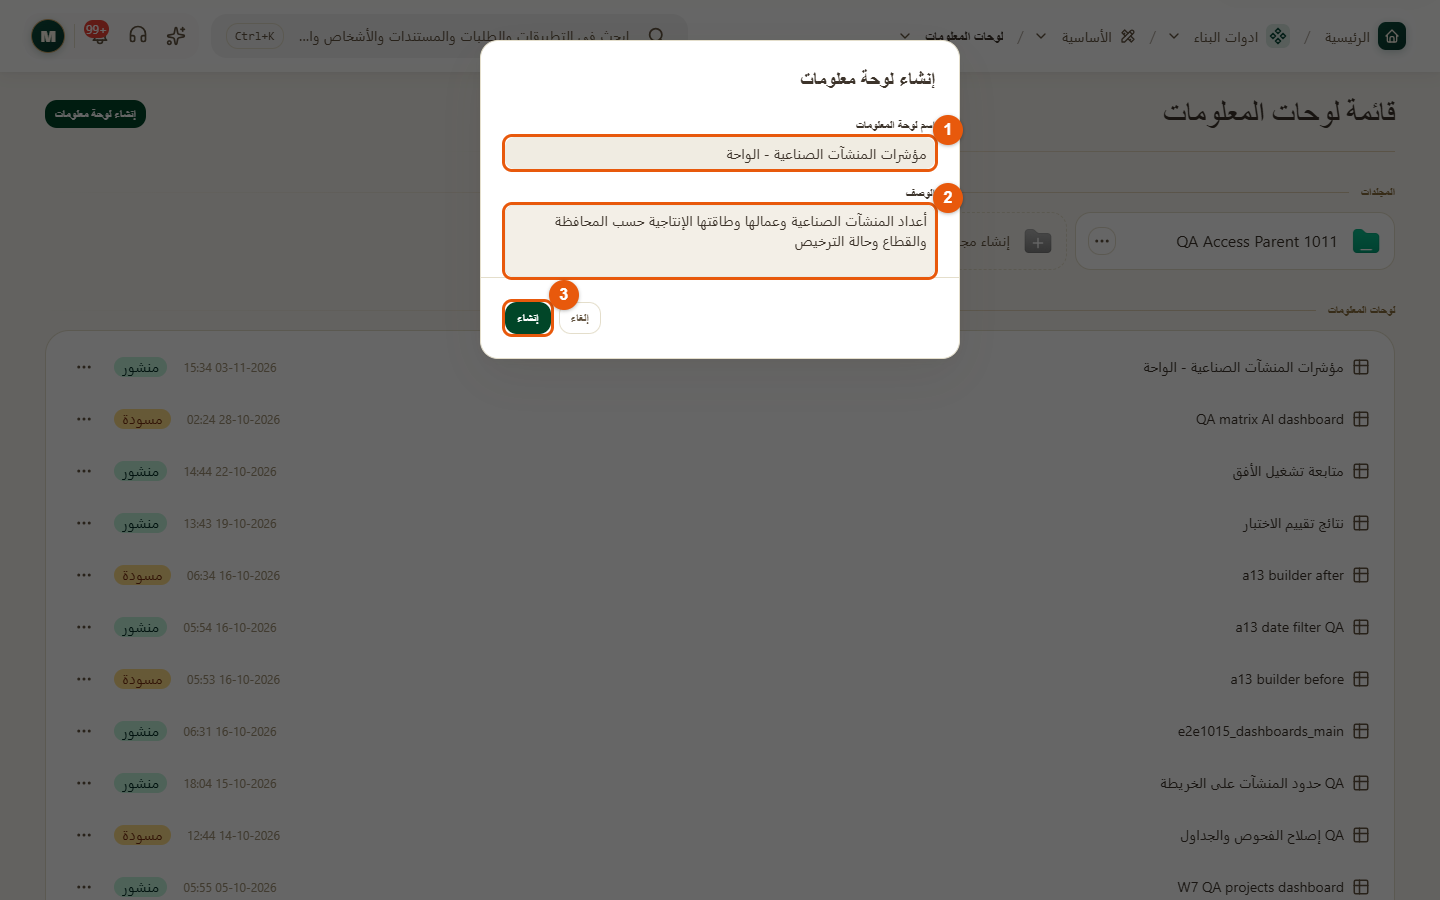
\includegraphics[width=0.62\linewidth]{assets/screens/i-new.png}
\caption{إنشاء لوحة معلومات}
\label{fig:build-dashboard-new}
\shotnote{صورة توضيحية من التنفيذ السابق؛ اتبع العلامات المرقّمة، واستخدم أسماء منظمتك وقيمها الواردة في النص بدلاً من بيانات الصورة. تطلب النافذة الاسم والوصف فقط، ثم تفتح محرر اللوحة مباشرة. ① «اسم لوحة المعلومات». ② «الوصف»: يظهر تحت الاسم لمن يفتح اللوحة. ③ «إنشاء».}
\end{figure}

\begin{figure}[H]
\centering
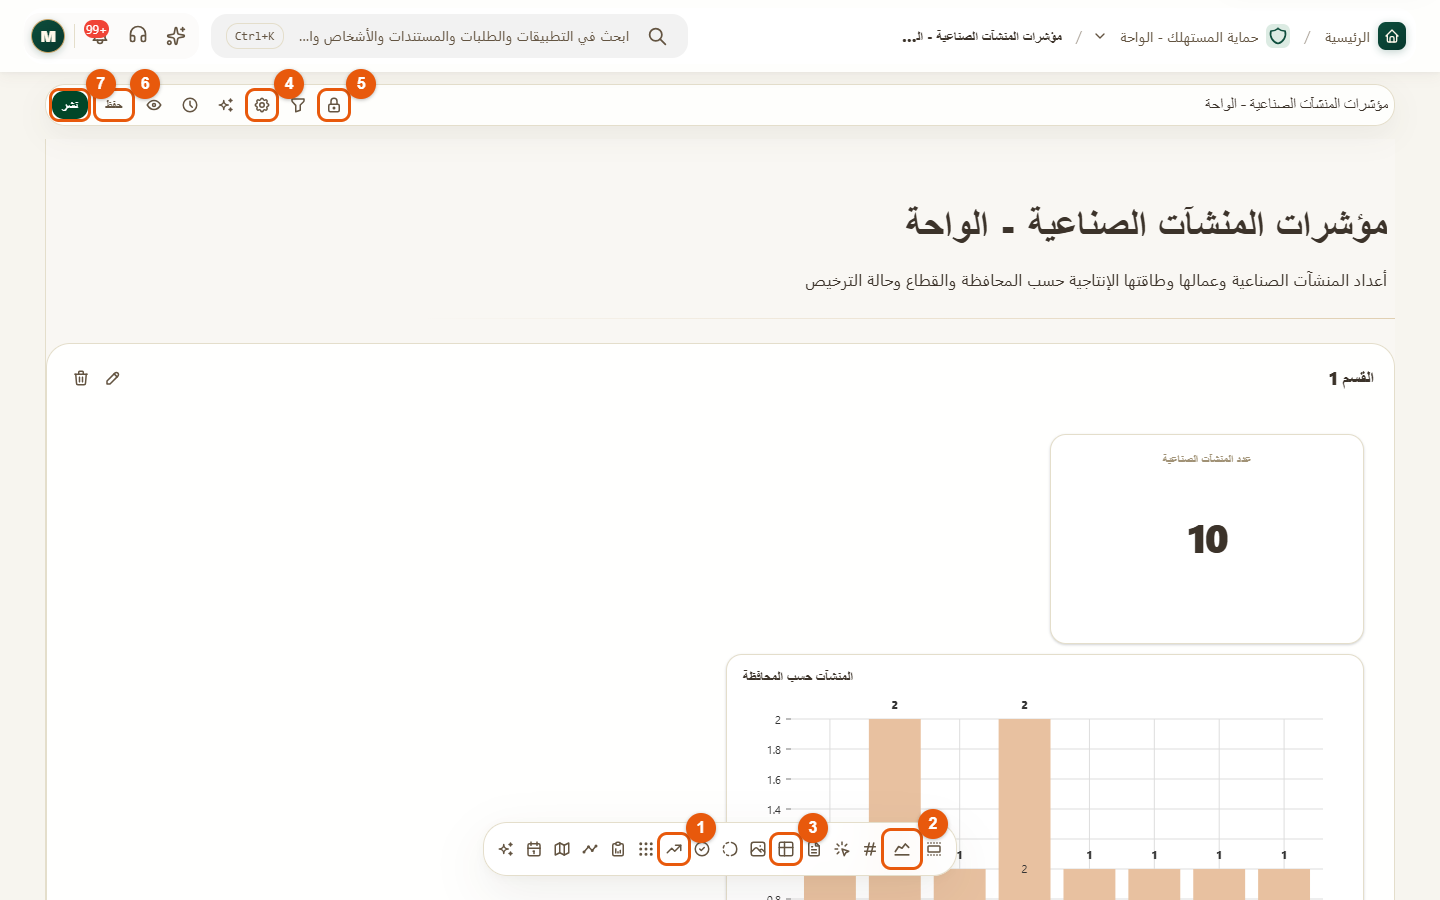
\includegraphics[width=0.95\linewidth]{assets/screens/i-builder.png}
\caption{محرر اللوحة}
\label{fig:build-dashboard-builder}
\shotnote{صورة توضيحية من التنفيذ السابق؛ اتبع العلامات المرقّمة، واستخدم أسماء منظمتك وقيمها الواردة في النص بدلاً من بيانات الصورة. يضيف الشريط السفلي العناصر، ويضبط الشريط العلوي اللوحة كلها. ① «مؤشر أداء»: رقم واحد. ② «إضافة رسم بياني (Nivo)»: أعمدة أو دائري وغيرهما. ③ «جدول». ④ «الإعدادات»: الاسم والتطبيق والقسم. ⑤ «إدارة الوصول»: من يرى اللوحة. ⑥ «حفظ». ⑦ «نشر»: لا يرى المشاهدون أي تعديل قبله.}
\end{figure}

\begin{enumerate}
\item افتح «ادوات البناء» ← «لوحات المعلومات» ← «إنشاء لوحة معلومات».
\item اكتب الاسم والوصف، ثم اضغط «إنشاء».
\end{enumerate}

\textbf{تحقق:} طابق النتيجة مع مصدر بياناتك وتصفية العنصر وصلاحيات المشاهد. القيم وأسماء المنشآت الصناعية في الصور بيانات تدريب سابقة، وليست بيانات منظمتك.

\subsection{اربط المؤشرات بنوع السجلات}

\begin{figure}[H]
\centering
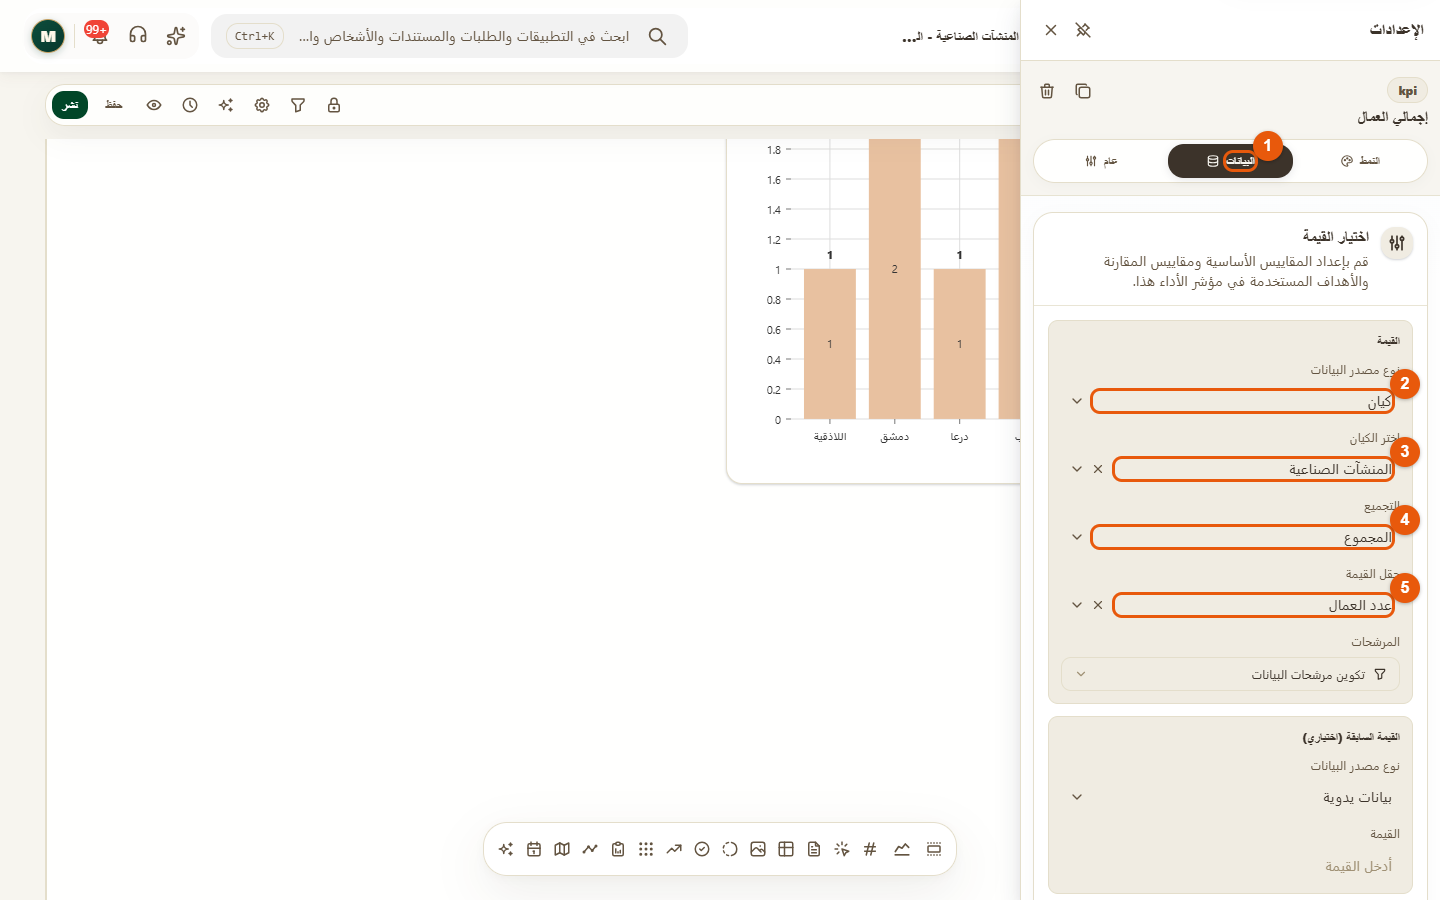
\includegraphics[width=0.95\linewidth]{assets/screens/i-kpi.png}
\caption{مصدر بيانات مؤشر الأداء}
\label{fig:build-kpi}
\shotnote{صورة توضيحية من التنفيذ السابق؛ اتبع العلامات المرقّمة، واستخدم أسماء منظمتك وقيمها الواردة في النص بدلاً من بيانات الصورة. يعيد العنصر حساب رقمه فور تغيير أي إعداد، فترى النتيجة قبل الحفظ. ① «البيانات». ② «نوع مصدر البيانات»: «كيان». ③ «اختر الكيان». ④ «التجميع»: «العدد» أو «المجموع» أو «المتوسط» أو الحد الأدنى أو الأقصى. ⑤ «حقل القيمة»: الحقل الرقمي الذي يُجمع.}
\end{figure}

\begin{enumerate}
\item اضغط «مؤشر أداء» في الشريط السفلي، فيُضاف العنصر وتُفتح إعداداته.
\item في «البيانات» ← «القيمة»: اختر «كيان»، ثم نوع السجلات، ثم «التجميع»، ثم «حقل القيمة» إن لزم.
\item افتح «عام»، واكتب «العنوان»، واضبط «العرض» و«الارتفاع». فالعرض 3 والارتفاع 2 يناسبان المؤشر.
\item أغلق الإعدادات، واضغط «حفظ».
\end{enumerate}

\textbf{تحقق:} طابق النتيجة مع مصدر بياناتك وتصفية العنصر وصلاحيات المشاهد. القيم وأسماء المنشآت الصناعية في الصور بيانات تدريب سابقة، وليست بيانات منظمتك.

\subsection{أضف الرسوم البيانية والجدول}

\begin{figure}[H]
\centering
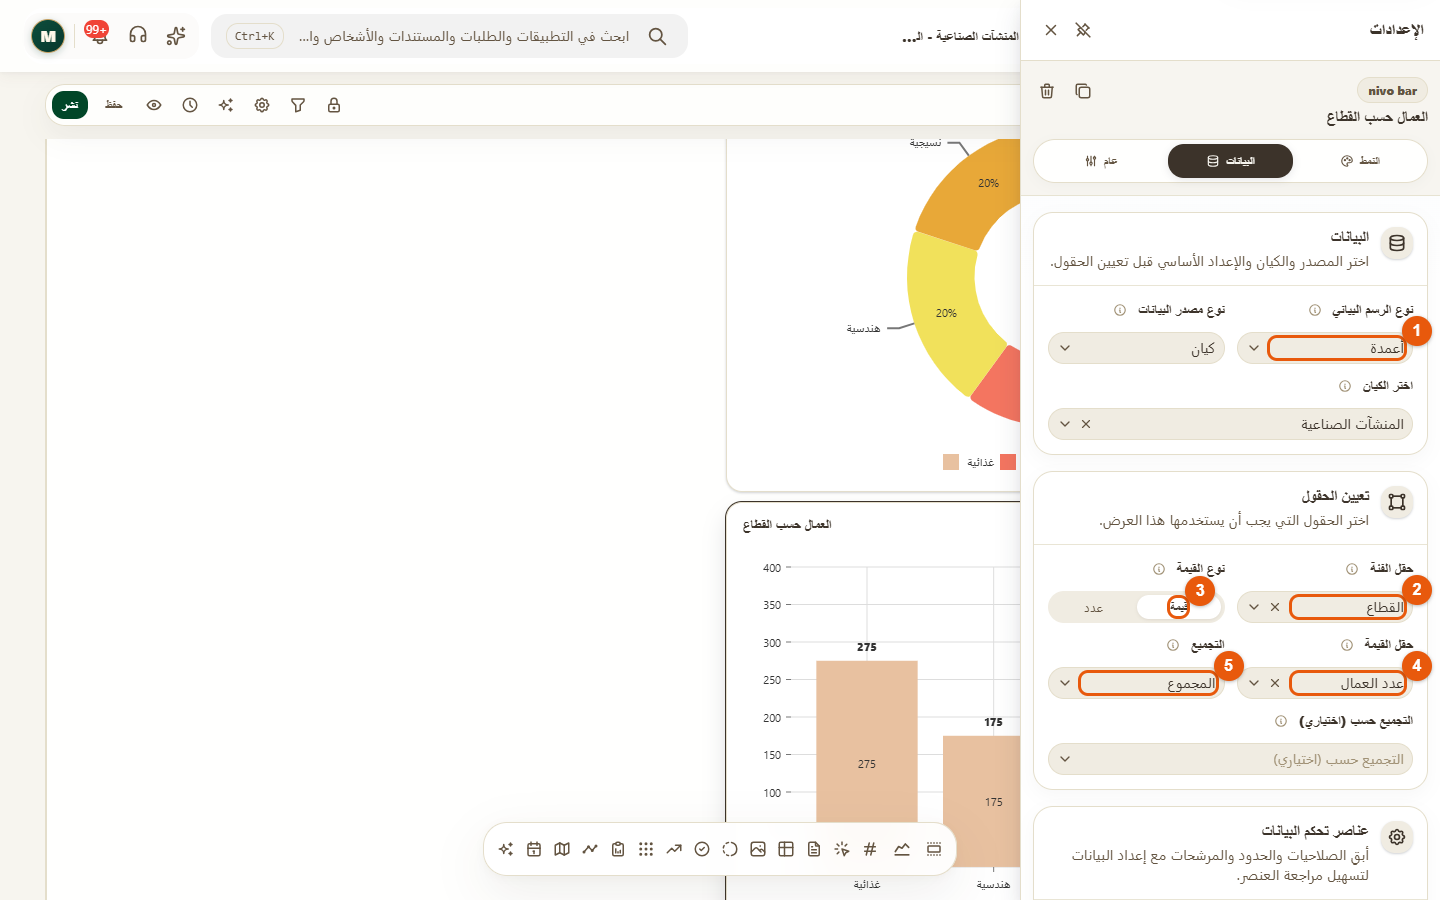
\includegraphics[width=0.95\linewidth]{assets/screens/i-bar.png}
\caption{ربط حقول رسم الأعمدة}
\label{fig:build-bar}
\shotnote{صورة توضيحية من التنفيذ السابق؛ اتبع العلامات المرقّمة، واستخدم أسماء منظمتك وقيمها الواردة في النص بدلاً من بيانات الصورة. يرسم العنصر بيانات تجريبية حتى تختار «كيان»، ثم يرسم سجلاتك. ① «نوع الرسم البياني». ② «حقل الفئة»: ما يظهر تحت الأعمدة. ③ «نوع القيمة»: «عدد» أو «قيمة». ④ «حقل القيمة». ⑤ «التجميع».}
\end{figure}

\begin{figure}[H]
\centering
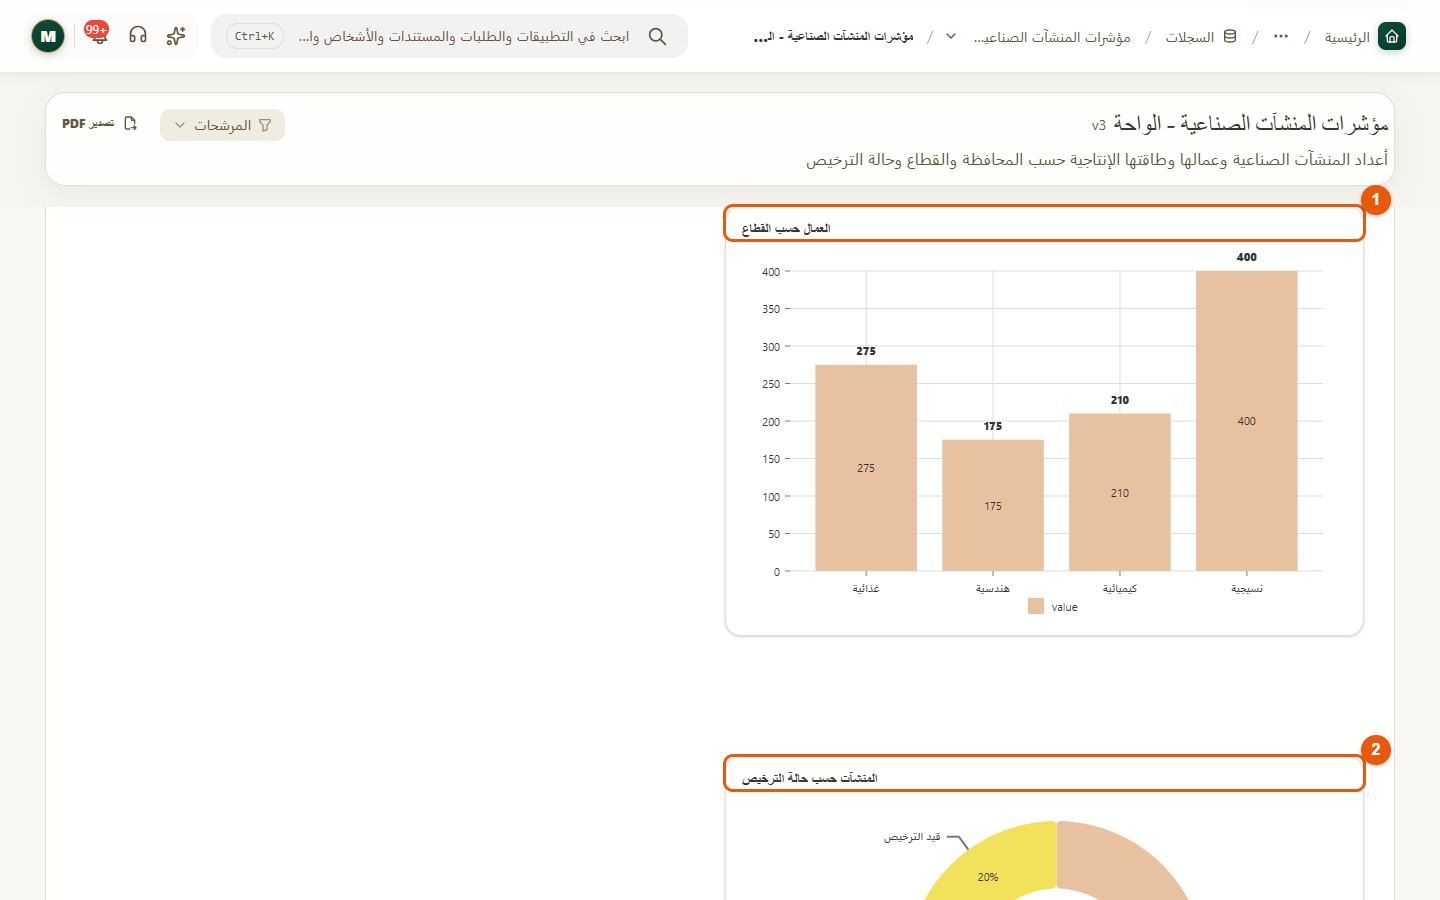
\includegraphics[width=0.95\linewidth]{assets/screens/i-view2.png}
\caption{الرسمان كما يراهما المشاهد}
\label{fig:build-charts-view}
\shotnote{صورة توضيحية من التنفيذ السابق؛ اتبع العلامات المرقّمة، واستخدم أسماء منظمتك وقيمها الواردة في النص بدلاً من بيانات الصورة. يكتب الرسم القيمة فوق كل عمود، ويكتب الرسم الدائري النسبة على كل جزء. ① «العمال حسب القطاع». ② «المنشآت حسب حالة الترخيص».}
\end{figure}

\begin{figure}[H]
\centering
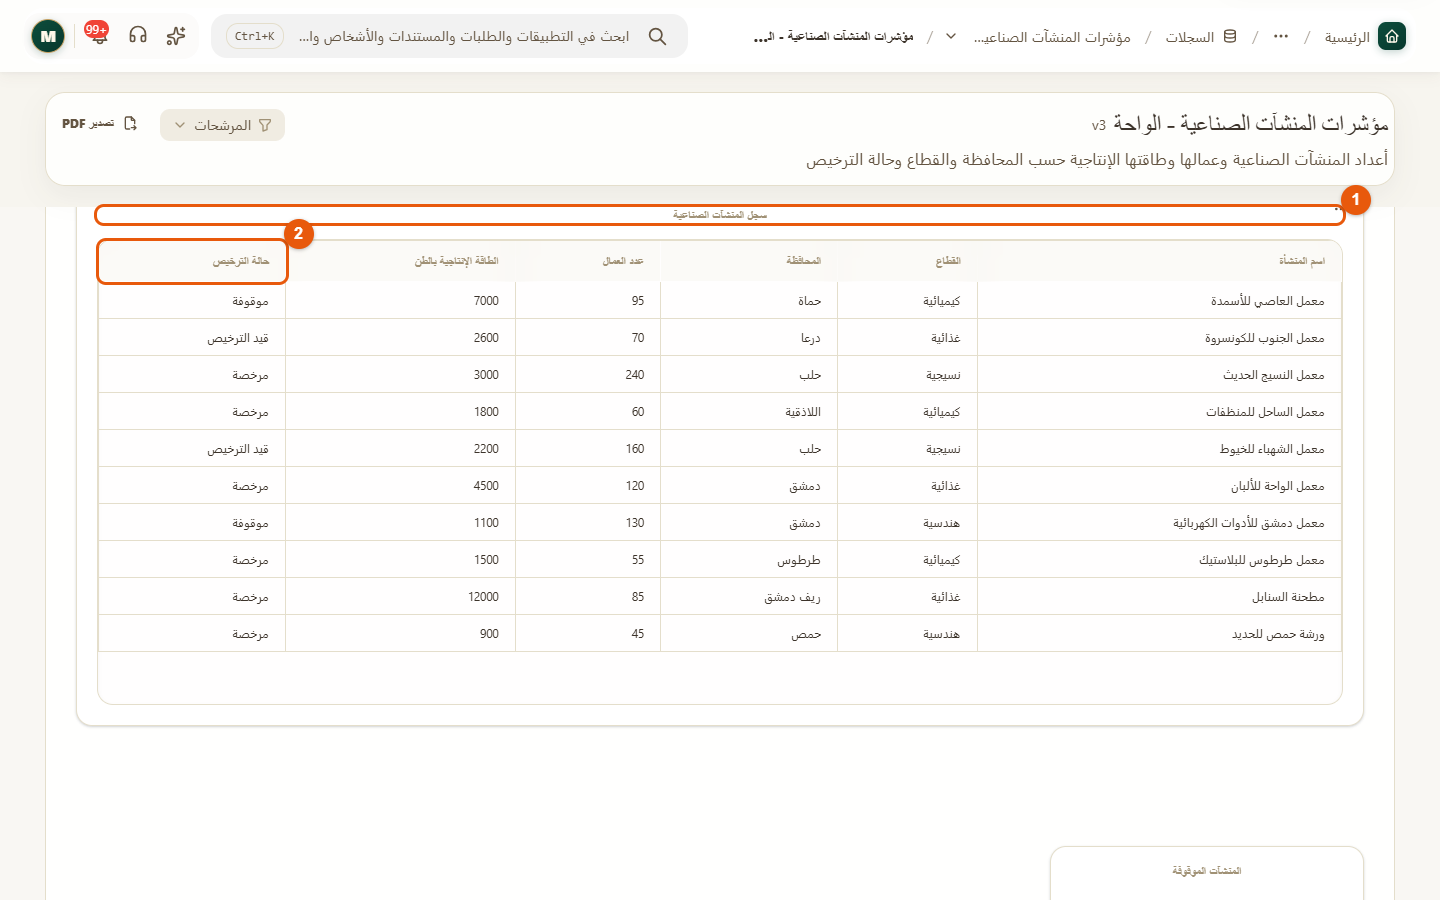
\includegraphics[width=0.95\linewidth]{assets/screens/i-view3.png}
\caption{جدول المنشآت}
\label{fig:build-table}
\shotnote{صورة توضيحية من التنفيذ السابق؛ اتبع العلامات المرقّمة، واستخدم أسماء منظمتك وقيمها الواردة في النص بدلاً من بيانات الصورة. يعرض الجدول السجلات نفسها التي تُحسب منها الأرقام، فيستطيع المشاهد أن يتحقق منها. ① عنوان الجدول. ② عمود «حالة الترخيص».}
\end{figure}

\begin{enumerate}
\item اضغط «إضافة رسم بياني (Nivo)»، واختر «أعمدة» أو «دائري».
\item في «البيانات» اختر «كيان»، ثم نوع السجلات، ثم «حقل الفئة».
\item للأعمدة اختر «نوع القيمة»: «عدد» للعدّ، أو «قيمة» ثم «حقل القيمة» ثم «التجميع». واختر الفئة أولاً؛ فتغييرها بعد ذلك يفرغ «حقل القيمة».
\item للجدول اضغط «جدول»، واختر «كيان» ونوع السجلات، ثم حدّد الأعمدة في «اختر الحقول».
\item سمِّ كل عنصر من «عام»، ثم اضغط «حفظ».
\end{enumerate}

\textbf{تحقق:} طابق النتيجة مع مصدر بياناتك وتصفية العنصر وصلاحيات المشاهد. القيم وأسماء المنشآت الصناعية في الصور بيانات تدريب سابقة، وليست بيانات منظمتك.

\subsection{احسب عدداً بشرط}

\begin{figure}[H]
\centering
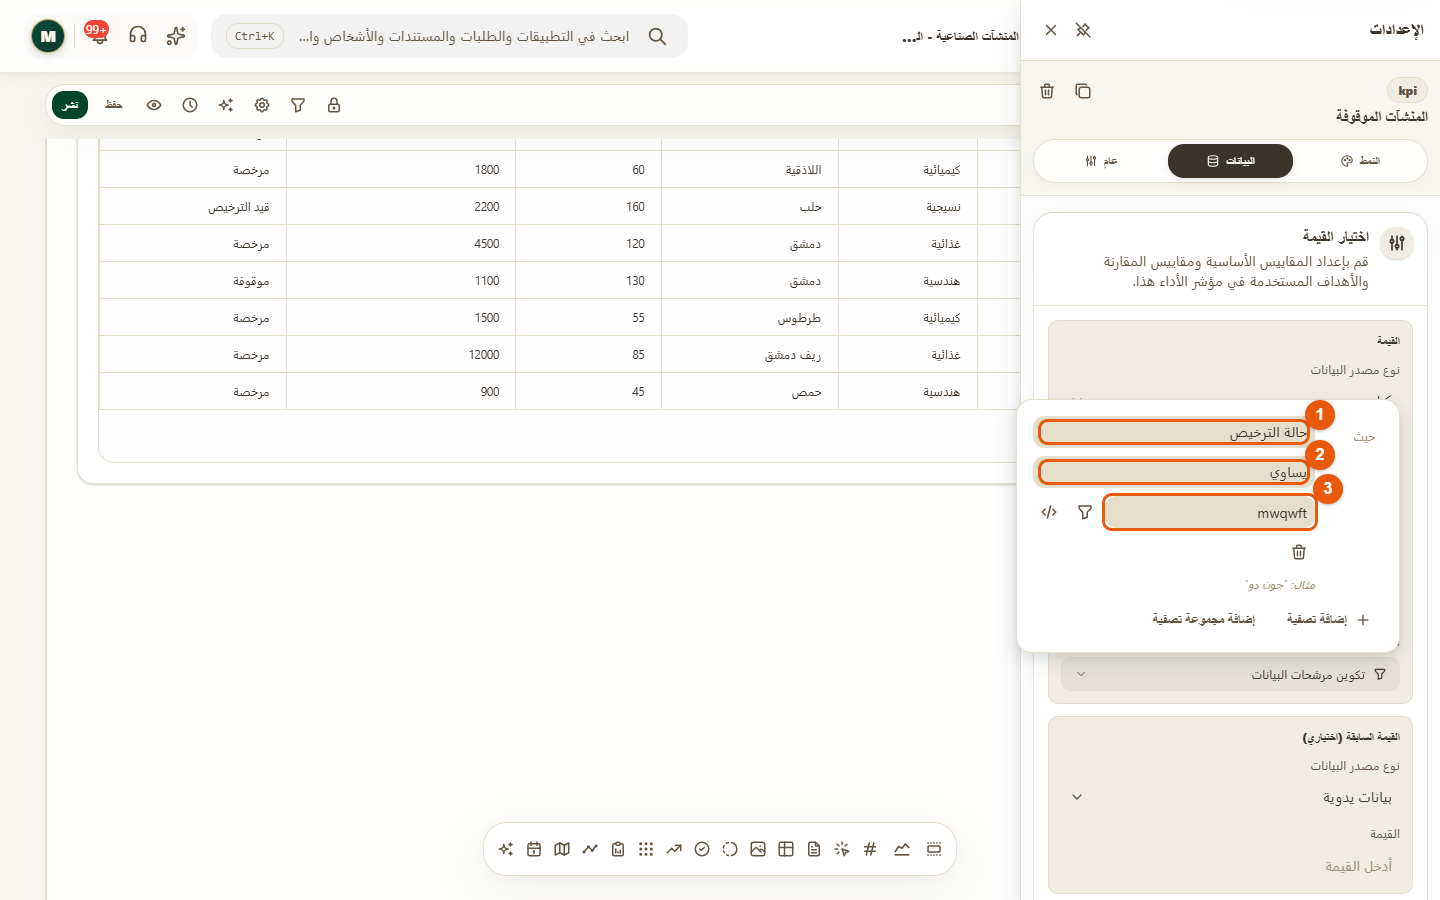
\includegraphics[width=0.95\linewidth]{assets/screens/i-wfilter.png}
\caption{تصفية داخل العنصر}
\label{fig:build-widget-filter}
\shotnote{صورة توضيحية من التنفيذ السابق؛ اتبع العلامات المرقّمة، واستخدم أسماء منظمتك وقيمها الواردة في النص بدلاً من بيانات الصورة. يُكتب المفتاح كما هو بلا علامتي تنصيص، لأن الحقل قيمة لا تعبير. ① الحقل. ② «يساوي». ③ القيمة: مفتاح الخيار.}
\end{figure}

\begin{enumerate}
\item اعرف مفتاح الخيار: افتح نوع السجلات ← «الحقول» ← الحقل، فيظهر المفتاح بجانب كل خيار في «الاختيارات».
\item في «البيانات» تحت «المرشحات»، اضغط «تكوين مرشحات البيانات» ← «إضافة تصفية».
\item اختر الحقل، واترك «يساوي»، واكتب المفتاح في «القيمة».
\end{enumerate}

\textbf{تحقق:} طابق النتيجة مع مصدر بياناتك وتصفية العنصر وصلاحيات المشاهد. القيم وأسماء المنشآت الصناعية في الصور بيانات تدريب سابقة، وليست بيانات منظمتك.

\subsection{اربط اللوحة بالتطبيق وشاركها ثم انشر}

\begin{figure}[H]
\centering
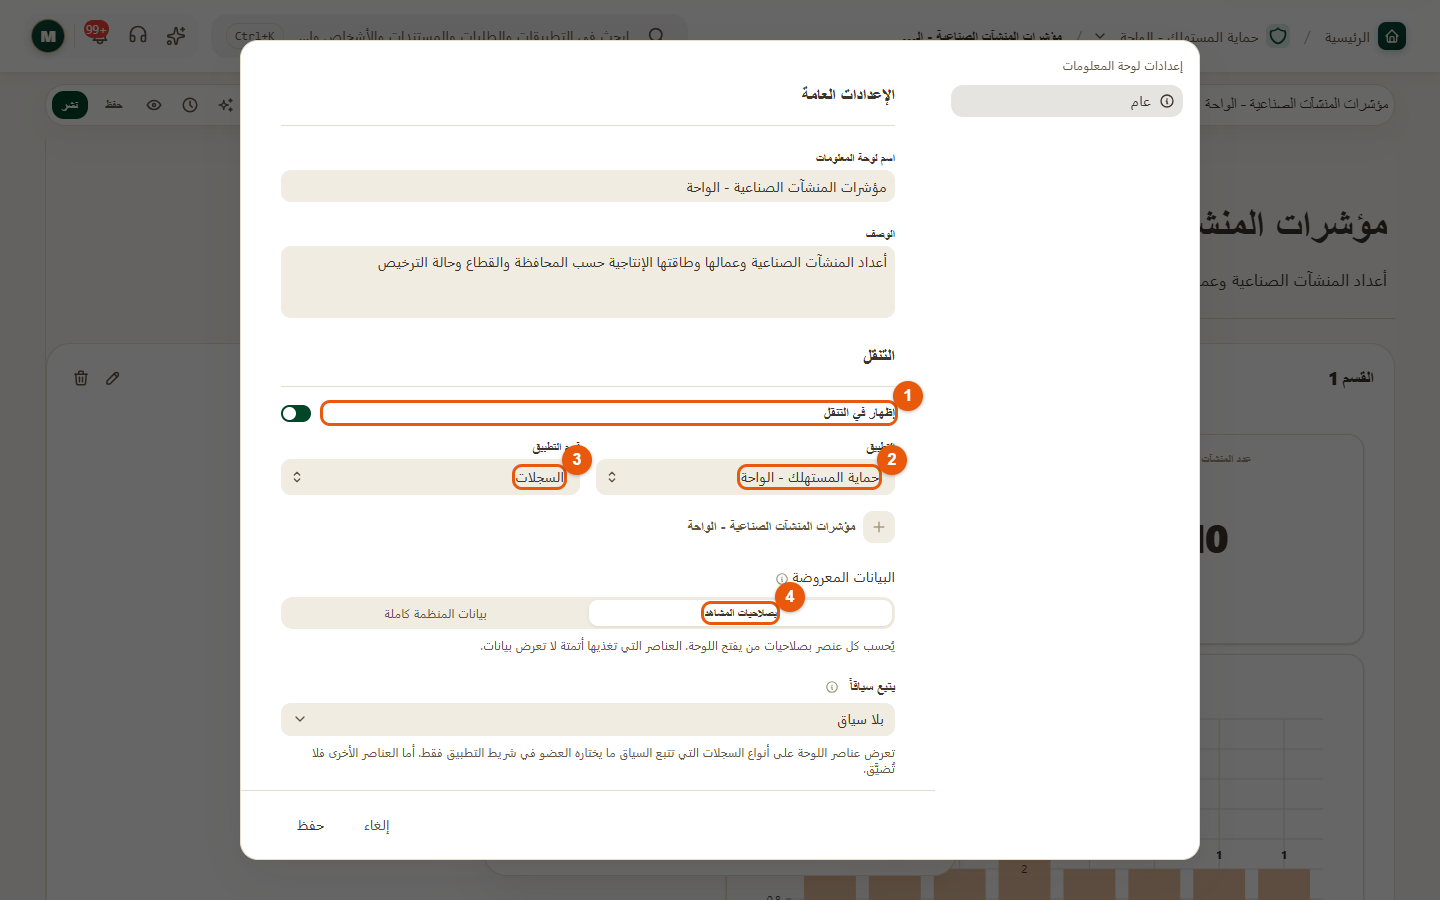
\includegraphics[width=0.95\linewidth]{assets/screens/i-settings.png}
\caption{مكان اللوحة في التطبيق}
\label{fig:build-dashboard-settings}
\shotnote{صورة توضيحية من التنفيذ السابق؛ اتبع العلامات المرقّمة، واستخدم أسماء منظمتك وقيمها الواردة في النص بدلاً من بيانات الصورة. يظهر التطبيق والقسم بعد تفعيل الإظهار فقط، كما في نوع السجلات. ① «إظهار في التنقل». ② «التطبيق». ③ «قسم التطبيق». ④ «البيانات المعروضة»: «بصلاحيات المشاهد» يحسب كل عنصر بصلاحيات من يفتح اللوحة.}
\end{figure}

\begin{figure}[H]
\centering
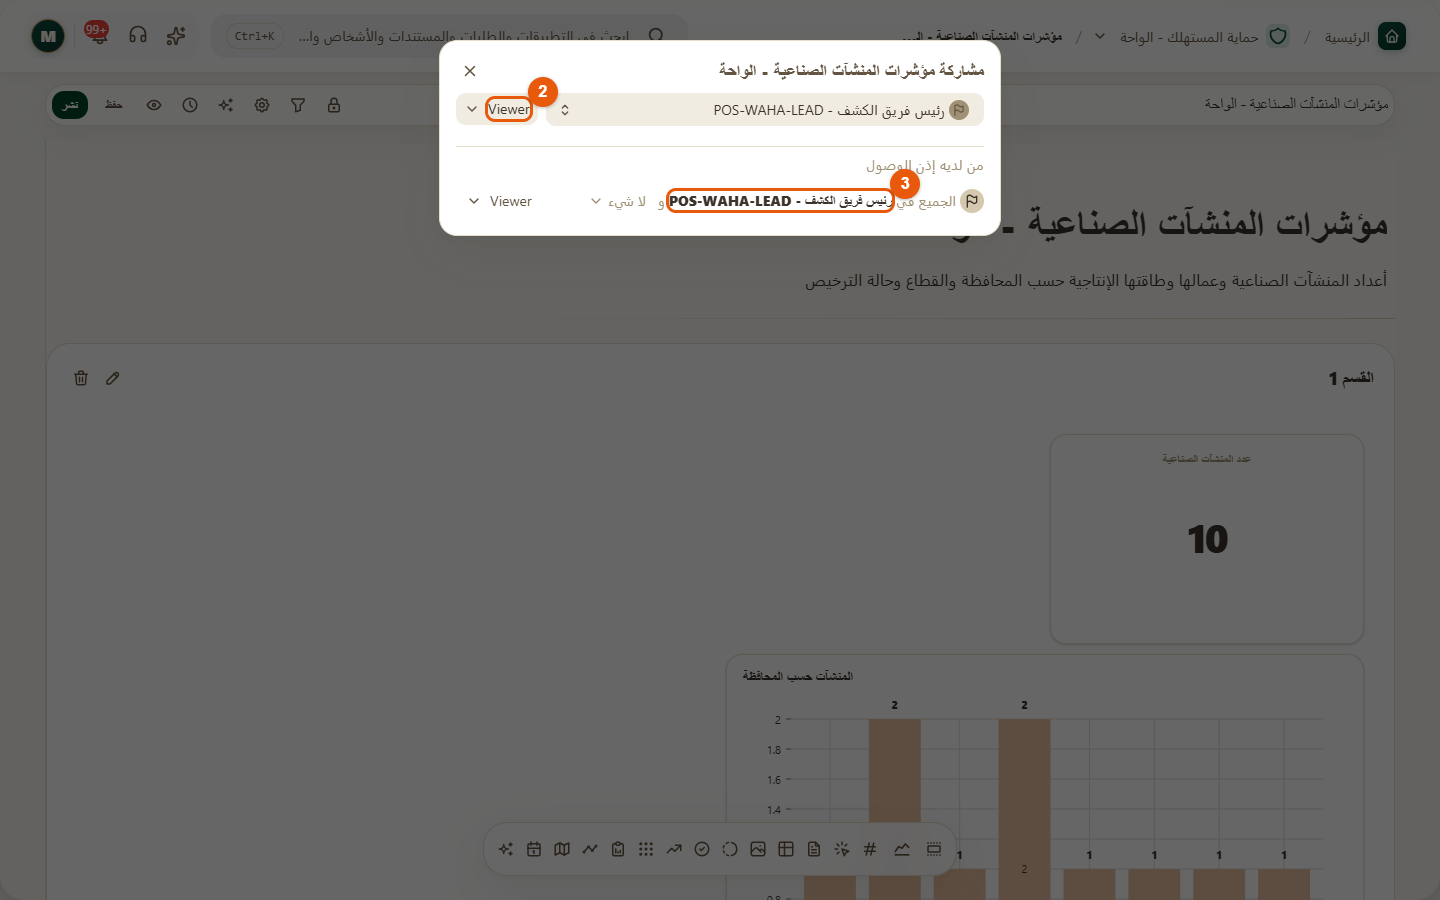
\includegraphics[width=0.62\linewidth]{assets/screens/i-share.png}
\caption{مشاركة اللوحة}
\label{fig:build-dashboard-share}
\shotnote{صورة توضيحية من التنفيذ السابق؛ اتبع العلامات المرقّمة، واستخدم أسماء منظمتك وقيمها الواردة في النص بدلاً من بيانات الصورة. تُشارك اللوحة مع منصب أو عضو أو مجموعة، كما يُسند الدور. ① حقل الاختيار. ② مستوى الوصول: \en{Viewer} للمشاهدة فقط. ③ المنصب الذي شوركت معه.}
\end{figure}

\begin{figure}[H]
\centering
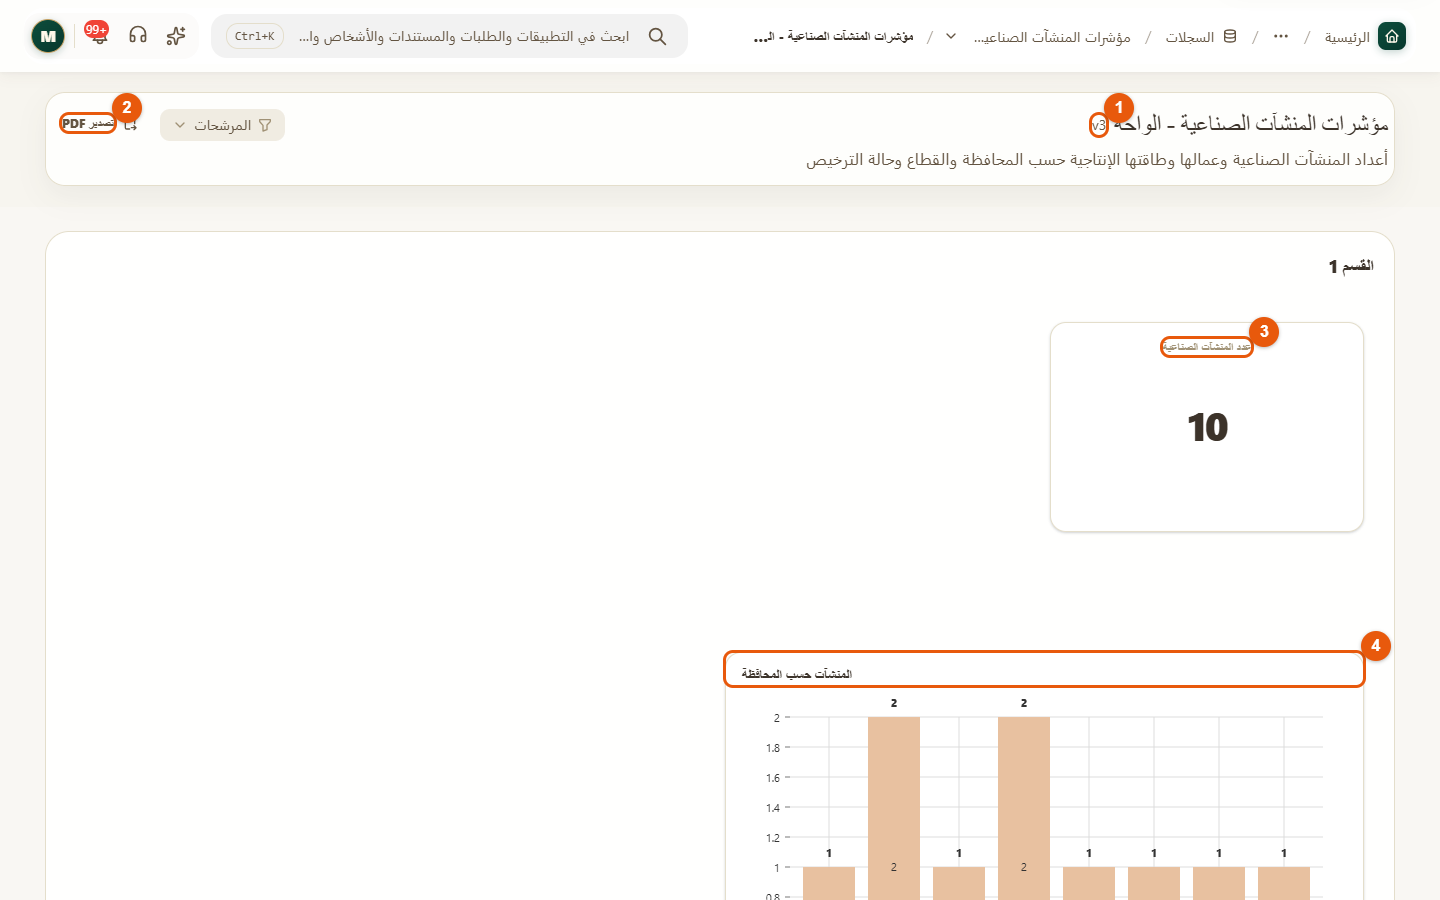
\includegraphics[width=0.95\linewidth]{assets/screens/i-view.png}
\caption{اللوحة بحساب رئيس الفريق}
\label{fig:build-dashboard-view}
\shotnote{صورة توضيحية من التنفيذ السابق؛ اتبع العلامات المرقّمة، واستخدم أسماء منظمتك وقيمها الواردة في النص بدلاً من بيانات الصورة. هذه اللوحة كما يفتحها رئيس الفريق من التطبيق، وأرقامها مطابقة لما في المحرر. ① رقم الإصدار المنشور: إذا ظهر رقم قديم، فلم تُنشر آخر التعديلات. ② «تصدير PDF». ③ «عدد المنشآت الصناعية». ④ «المنشآت حسب المحافظة».}
\end{figure}

\begin{enumerate}
\item اضغط «الإعدادات»، وفعّل «إظهار في التنقل»، واختر «التطبيق» و«قسم التطبيق»، واترك «بصلاحيات المشاهد»، ثم اضغط «حفظ».
\item اضغط «إدارة الوصول»، وابحث عن المنصب واختره، واترك المستوى \en{Viewer}.
\item افتح نوع السجلات ← «الصلاحيات»، وامنح دور المشاهد «قائمة» و«فتح»، ثم «المراجعة والنشر» ← «نشر».
\item اضغط «نشر» في اللوحة.
\end{enumerate}

\textbf{تحقق:} طابق النتيجة مع مصدر بياناتك وتصفية العنصر وصلاحيات المشاهد. القيم وأسماء المنشآت الصناعية في الصور بيانات تدريب سابقة، وليست بيانات منظمتك.

\section{عالج اختلاف ما تراه عن الدليل}
\label{sec:build-issues}

الأسماء والرموز هي نقطة البداية للتحقق، أما جاهزية التشغيل فتحتاج مراجعة العلاقات والصلاحيات والإعداد المنشور. لا تفسّر كل اختلاف على أنه سجل مفقود يجب إنشاؤه.

\begin{rcnote}[من منظمتك: حماية المستهلك]
إذا ظهر «مدقق كشوف المنشآت» في أكثر من موضع، فميّز الوصف الوظيفي عن الدور، وعن المنصب «مدقق كشوف المنشآت — 01». لكل واحد منها وظيفة مختلفة، حتى عندما تتشابه الأسماء.
\end{rcnote}

\begin{table}[H]
\centering
\caption{ما الذي تراجعه عند الاختلاف؟}
\label{tab:build-issues}
\begin{tabularx}{\linewidth}{R{4.2cm} Y}
\rcHeaderRow
\thh{ما ظهر} & \thh{التحقق والخطوة التالية}\\
اسم العضو أو المنصب مختلف & ابحث برقم الموظف أو رمز المنصب؛ احتفظ بلاحقة «تجريبي» والرقم 01.\\
تبعية المدقق مختلفة عن الباحث & المدقق يتبع لرئيس دائرة حماية المستهلك، والباحث لرئيس فريق الكشف؛ لا توحّد التبعيتين.\\
النموذج ليس في السجلات التجارية & موقعه الذي تمت مطابقته هو «حماية المستهلك» ← «السجلات».\\
المنشأة لا تظهر للحساب & راجع «قائمة» و«فتح» وإسناد الدور والنطاق، ثم إعدادات التنقل.\\
لا يوجد تكليف لنور & راجع وجود الخطة وحالتها ومرشحيها وتعيين نور؛ لا تستنتج الجاهزية من وجود النموذج.\\
الكشف لا يصل إلى ريم & راجع موقّع خطوة الموافقة وحالة البدء وإسناد الدور في النموذج.\\
اعتماد دون تحديث للمنشأة & راجع هل توجد كتابة أصلاً، وحالة السماح، والحقول والقيم، ونتيجة التنفيذ.\\
المؤشر مختلف عن القائمة & طابق المصدر والتصفية وحساب المشاهد؛ لا تستخدم أرقاماً من بيئة أخرى.\\
\end{tabularx}
\end{table}

\textbf{تحقق:} ينبغي أن تستطيع تتبّع الدائرة إلى المناصب والتعيينات، ثم النموذج والمنشأة، مع تمييز الإعداد الموجود عن أي إعداد لم يكتمل بعد. لم تتضمن مراجعة إعداد هذا الفصل اختبار إرسال أو اعتماد في المنظمة.
